\documentclass{article}
% Language setting
% Replace `english' with e.g. `spanish' to change the document language
\usepackage[english]{babel}

\usepackage{caption}
% Set page size and margins
% Replace `letterpaper' with `a4paper' for UK/EU standard size
\usepackage[letterpaper,top=2cm,bottom=2cm,left=3cm,right=3cm,marginparwidth=1.75cm,margin=1in]{geometry}
\usepackage{listings}

% Useful packages
\usepackage{amsmath}
\usepackage{graphicx}
\usepackage{subfig}
\usepackage{algorithm}
\usepackage{algpseudocode}

\usepackage{graphicx}
\usepackage{caption}
\usepackage{array}
\usepackage{booktabs}
\setlength{\heavyrulewidth}{1.5pt}
\setlength{\abovetopsep}{4pt}


\usepackage[colorlinks=true, allcolors=blue]{hyperref}

\title{3D Shape, Pre-processing and Visualization}
\author{Megan Mirnalini Sundaram R, Sherry Usman}

\begin{document}
\maketitle

\section*{Question 1}
\subsection*{Slices and Aspect Ratio}
The image has 16 slices. The aspect ratio can be defined as the ratio of total width (total number of columns) and the total height (total number of rows). In that case it is 160/140 which is 1.143. 

\subsection*{Function to display the contents of the 3D image} \label{sec:contents-3D_image}
The code snippet below shows the function for displaying the slices of the image.  
\begin{lstlisting}
import numpy as np
import matplotlib.pyplot as plt 

num_slices = 16
fig, axes = plt.subplots(4,4, figsize =(12,12))
for i in range(num_slices):
  ax = axes[i // 4, i % 4]
  tif.seek(i)
  slice = np.array(tif)

  ax.imshow(slice)
  ax.axis('off')
  ax.set_title(f'Slice {i+1}')

plt.tight_layout()
plt.show()
\end{lstlisting}
The results of this function are show in Appendix: Figure \ref{fig:3d-plane-image}. 
\clearpage
\section*{Question 2}
\subsection*{Thresholding and best value}
Thresholding was done on the chromo.tiff image using the \textit{diplib} library in Python and using VAA3D software.\\Figure \ref{fig:thresholding} shows the result of the Otsu Threshold (\ref{fig:otsu}) and the result of Otsu threshold with median filter (\ref{fig:median_otsu}). 

\begin{figure}[h!]
\centering
\subfloat{\label{fig:otsu}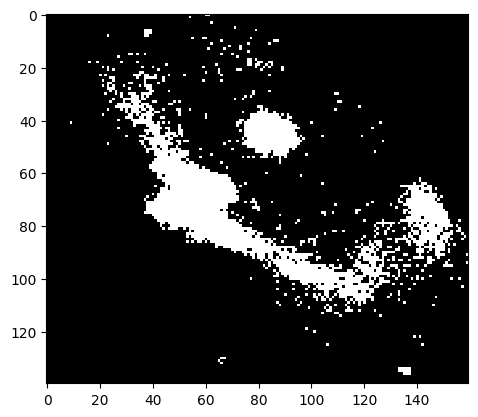
\includegraphics[width=0.5\textwidth]{Report/Images/otsu_threshold_image.png}}
\subfloat{\label{fig:median_otsu}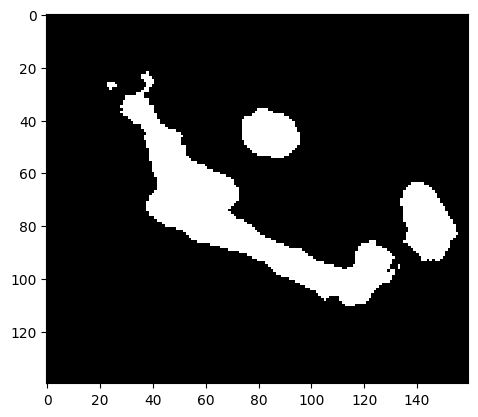
\includegraphics[width=0.5\textwidth]{Report/Images/median_filter.png}}
\caption{(a) Chromo.tiff with Otsu Threshold, and (b) Chromo.tiff with Median Filter and Otsu Threshold}
\label{fig:thresholding}
\end{figure}


Figure \ref{fig:vaa3dthresh} shows the result of the Vaa3D software. As seen in figure \ref{fig:vaa3dthresh}, the best threshold value is 55. 

\begin{figure}[h!]
    \centering
    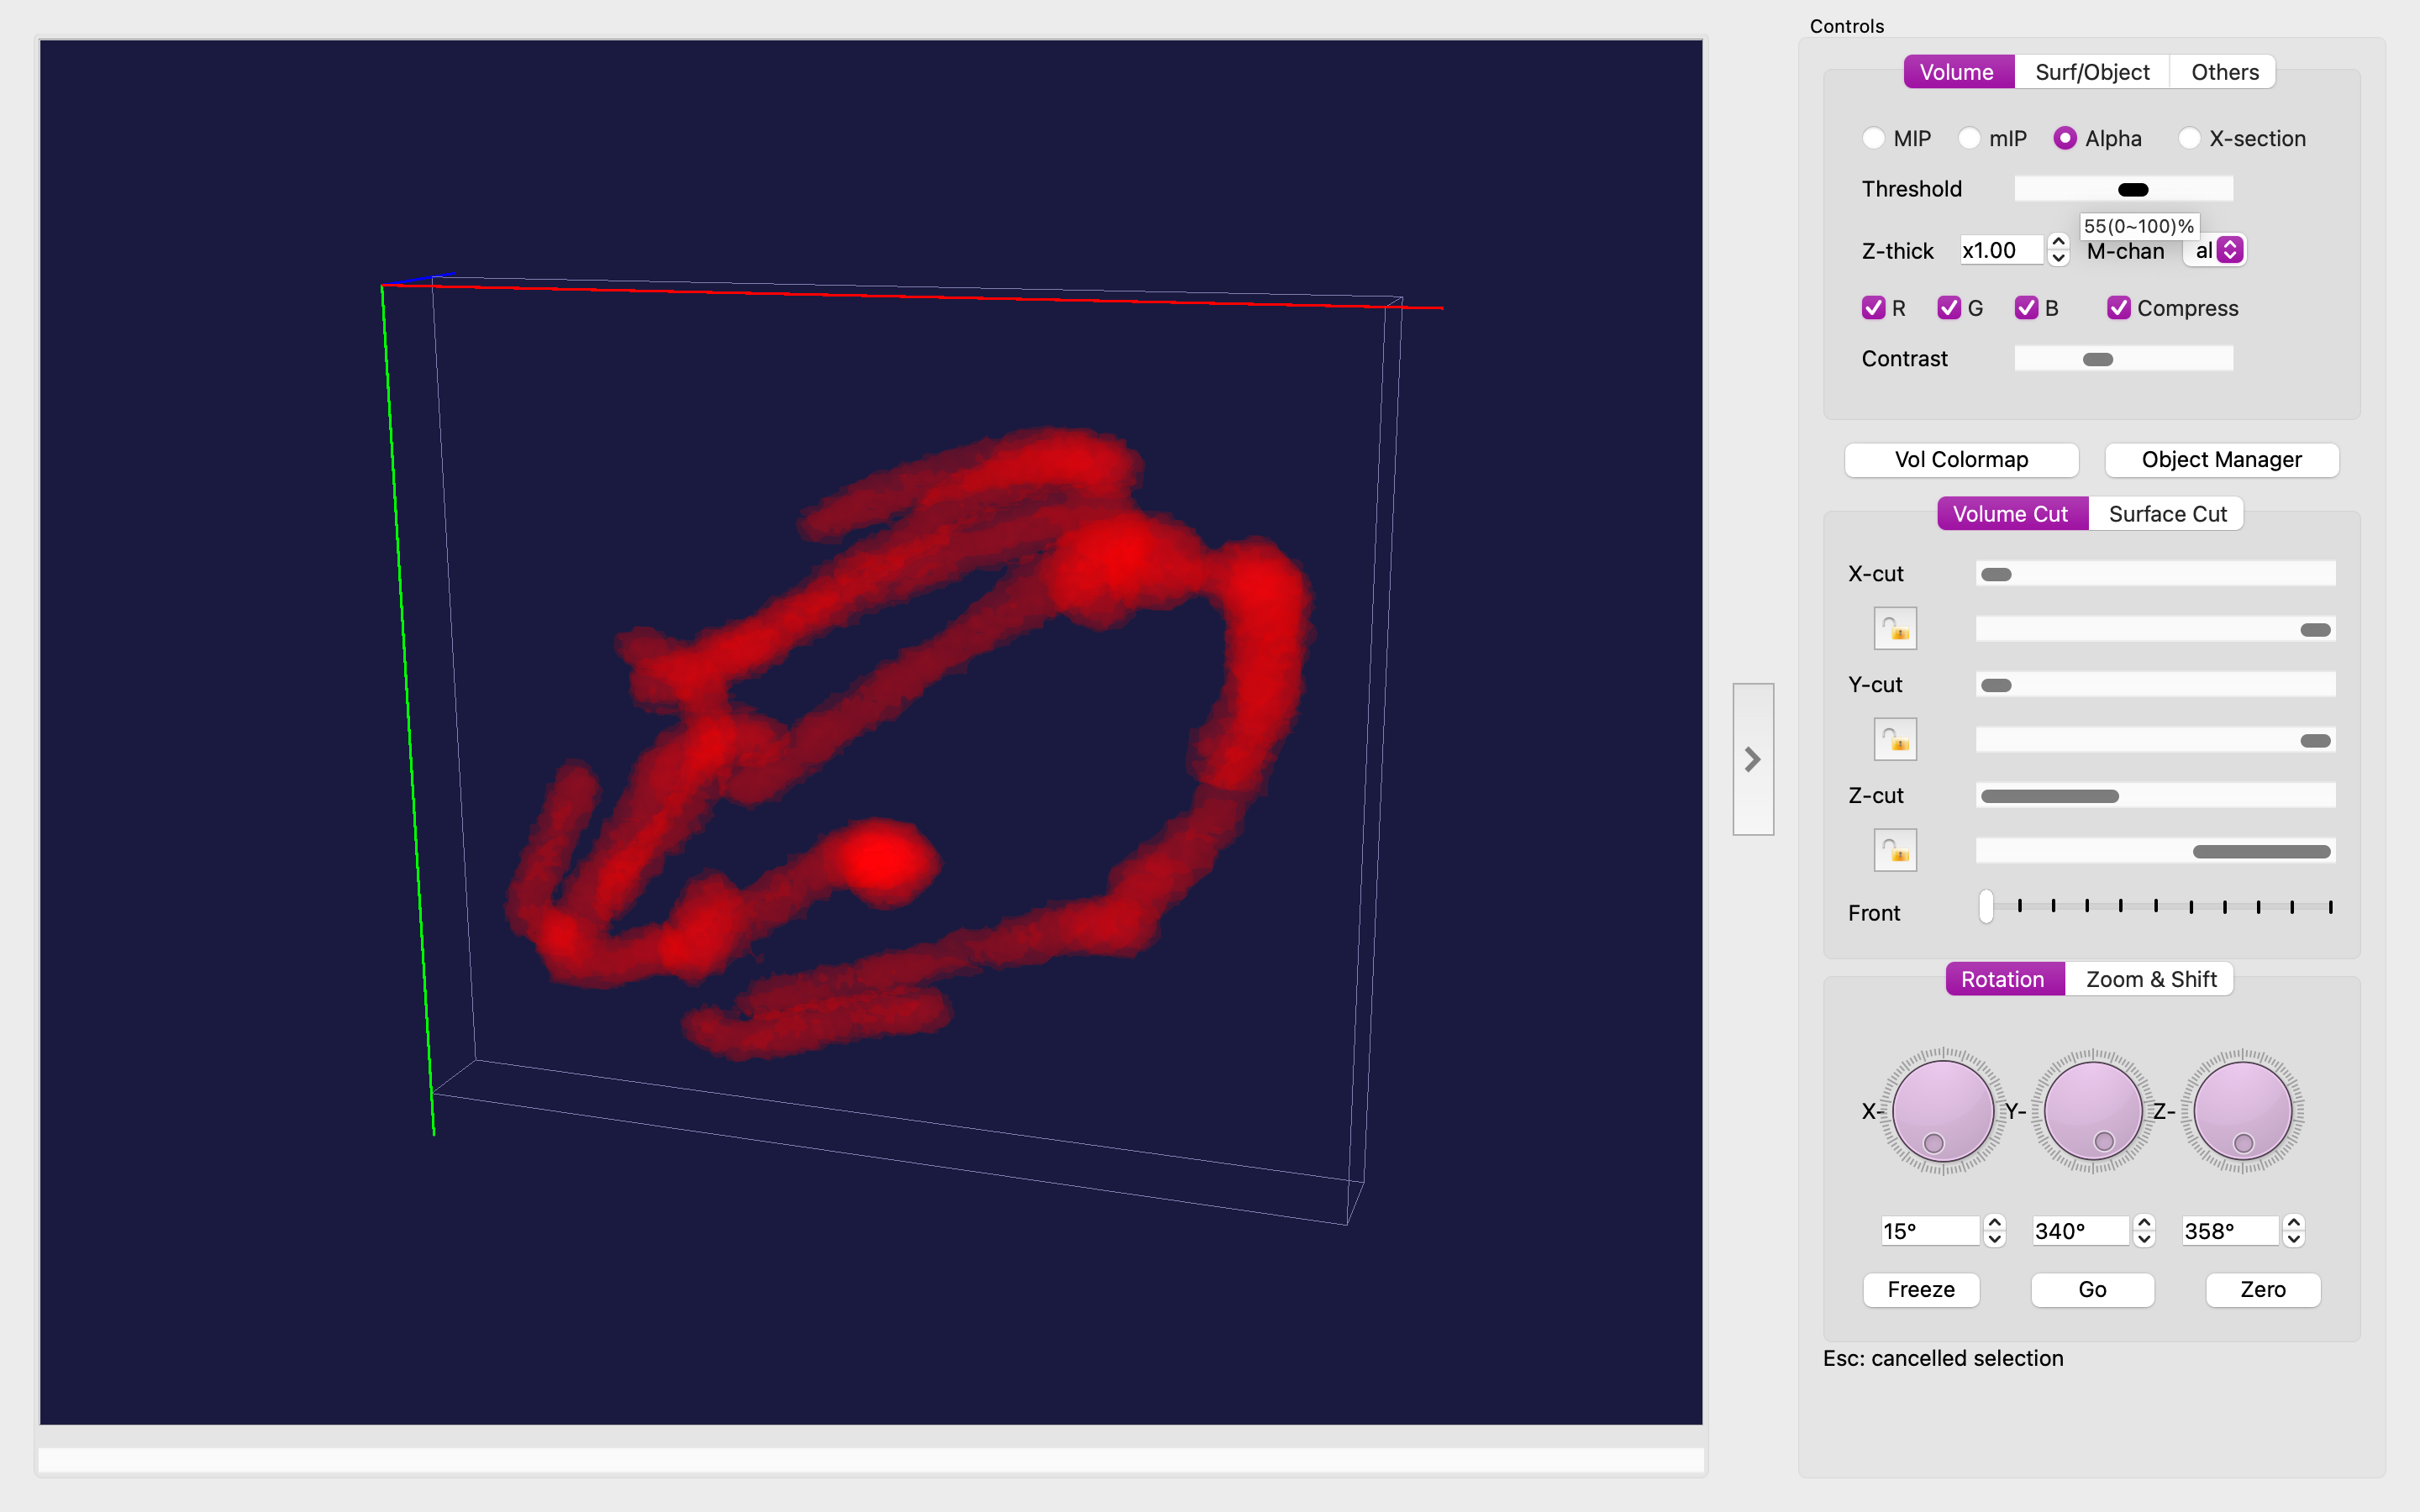
\includegraphics[width=1\linewidth]{Report/Images/vaa3d_thresh.png}
    \caption{Chromo.tiff image thresholded in VAA3D}
    \label{fig:vaa3dthresh}
\end{figure}



\subsection*{Algorithm for Depth Cueing}
The figure \ref{fig:depth-cuing} shows the algorithm for depth cueing. As shown in the algorithm, 16 evenly spaced values are taken from the range 0 to 255 and the slices are thresholded with the values. Slices lower in the plane are thresholded with lower values and slices higher in the plane are thresholded iwth higher values. The slices are combined to create a 3-dimensional layered image. 
\begin{figure}[h!]
    \centering
    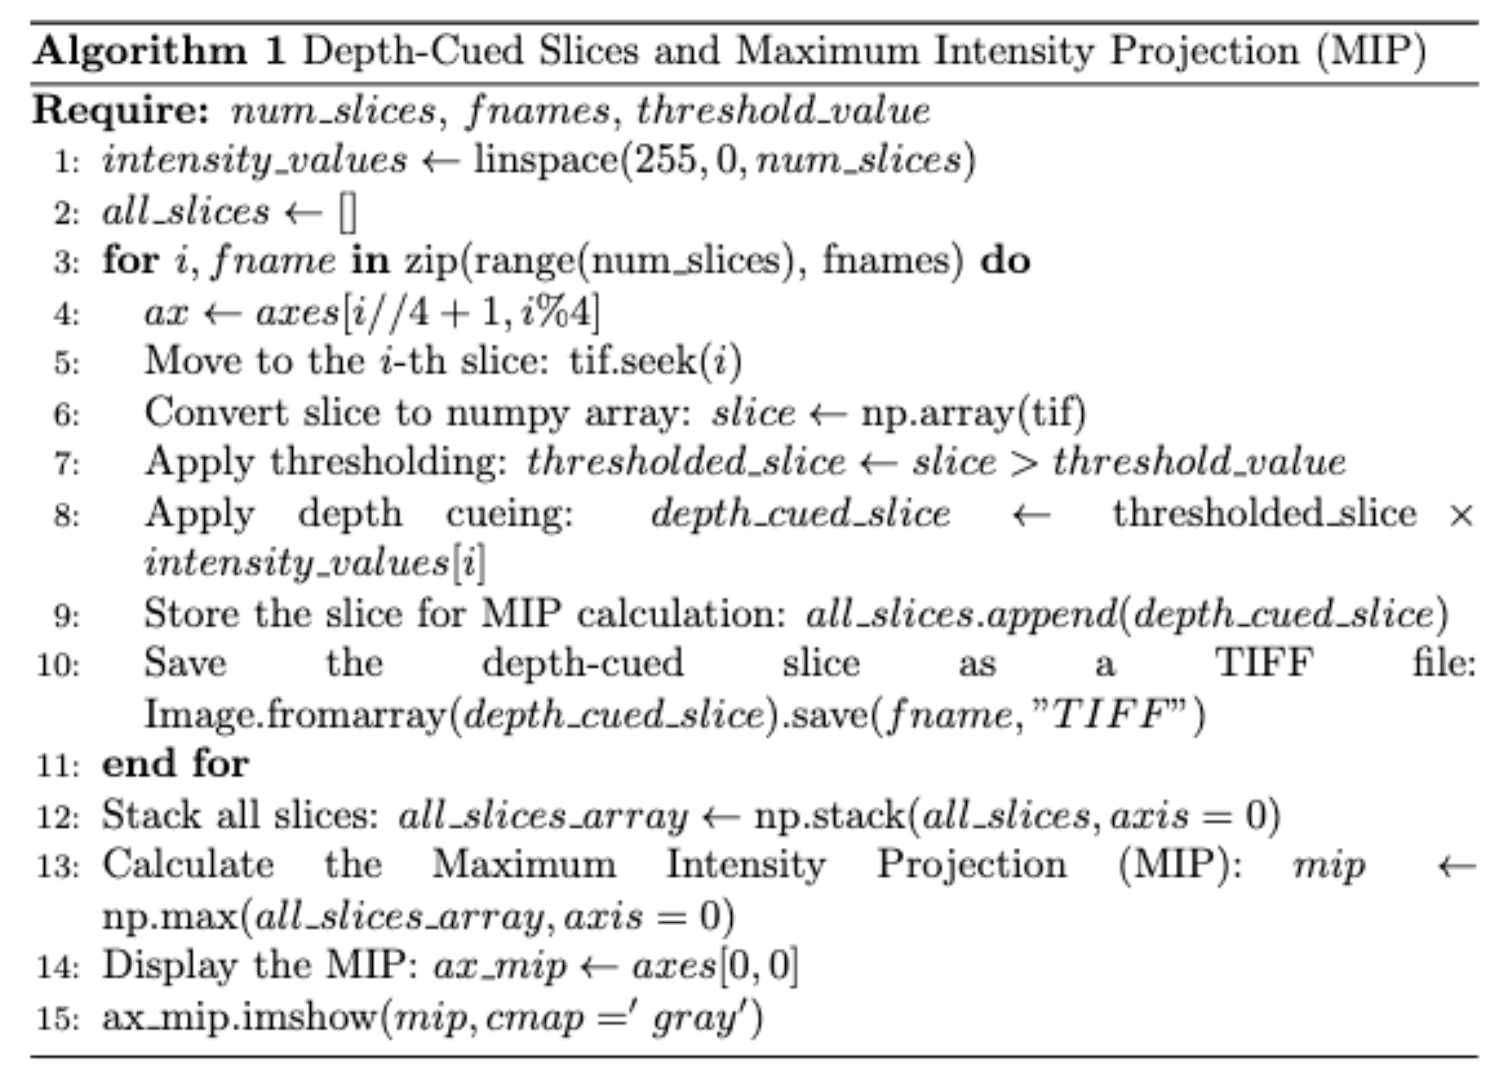
\includegraphics[width=0.8\linewidth]{Report/Images/depth_cuing.png}
    \caption{Algorithm for depth cueing }
    \label{fig:depth-cuing}
\end{figure}

\subsection*{Depth Cueing}
Figure \ref{fig:depth-cuing-results} shows the result of depth cueing. 
\begin{figure}[h!]
    \centering
    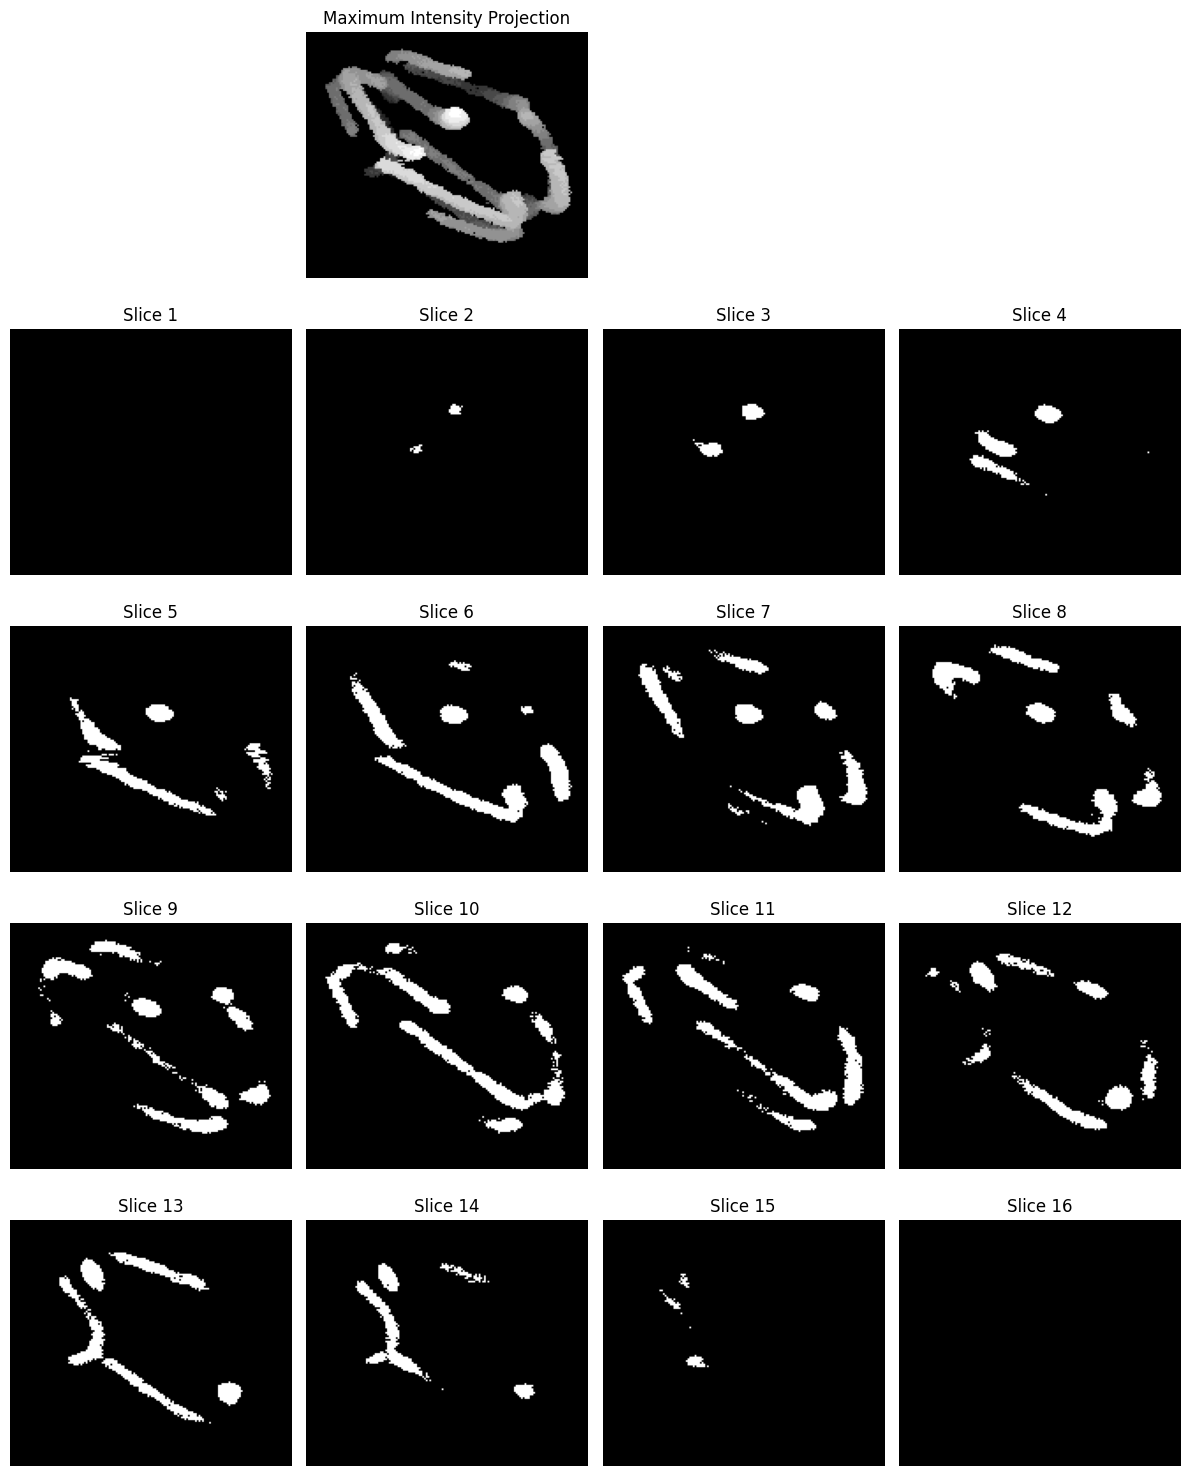
\includegraphics[width=1\linewidth]{Report/Images/mip.png}
    \caption{Chromo.tiff with depth cueing}
    \label{fig:depth-cuing-results}
\end{figure}

The first image is a raw image obtained before processing techniques such as thresholding, median filter and contrast stretching. Thus it looks out of focus, blurry and underexposed. The second image is the product of these image analysis methods and the original image. 

\begin{figure}[h!]
    \centering
    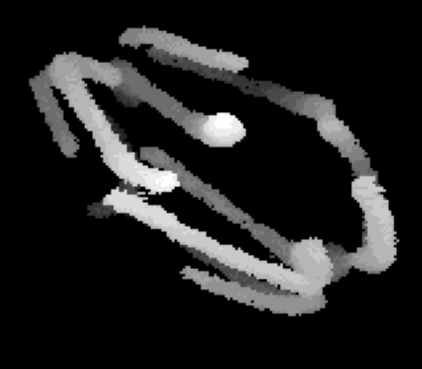
\includegraphics[width=0.5\linewidth]{Report/Images/max_intensity.png}
    \caption{The stacked result of MIP}
    \label{fig:mip}
\end{figure}

\clearpage
\section*{Question 3}
\subsection*{Maximum Projection and Alpha Function}
As instructed in the file, the contrast was varied. In addition to this, the thickness \textbf{Z-thick} was also varied, to understand the effect on the contrast. \\The video files were generated for both maximum projection and alpha function, and are submitted along with this file. 

\medskip

\textbf{Maximum Projection} : File Name - \textit{chromo-MIP\_Contrast.mp4}

\textbf{Alpha Projection} : File Name - \textit{chromo-Alpha\_Contrast.mp4}
\subsection*{Surface Visualization}
For the given image, the lower and upper ranges were varied between [0,75], [75,150] and [150,255]. In addition to varying the ranges, the mesh density was also varied between [25,50,75,100].
\begin{itemize}
    \item Figures \ref{fig:surface_vis_0_75-25}, \ref{fig:surface_vis_0_75-50}, \ref{fig:surface_vis_0_75-75} and \ref{fig:surface_vis_0_75-100} capture the results, when the lower range is 0 and the upper range is 75, with the mesh density as 25, 50, 75, 100 respectively. 
    \item Figures \ref{fig:surface_vis_75_150-25}, \ref{fig:surface_vis_75_150-50}, \ref{fig:surface_vis_75_150-75} and \ref{fig:surface_vis_75_150-100} capture the results, when the lower range is 75 and the upper range is 150, with the mesh density as 25, 50, 75, 100 respectively.
    \item Figures \ref{fig:surface_vis_150_255-25}, \ref{fig:surface_vis_150_255-50}, \ref{fig:surface_vis_150_255-75} and \ref{fig:surface_vis_150_255-100} capture the results, when the lower range is 150 and the upper range is 255, with the mesh density as 25, 50, 75, 100 respectively. 
\end{itemize}

\begin{figure}[h!]
    \centering
    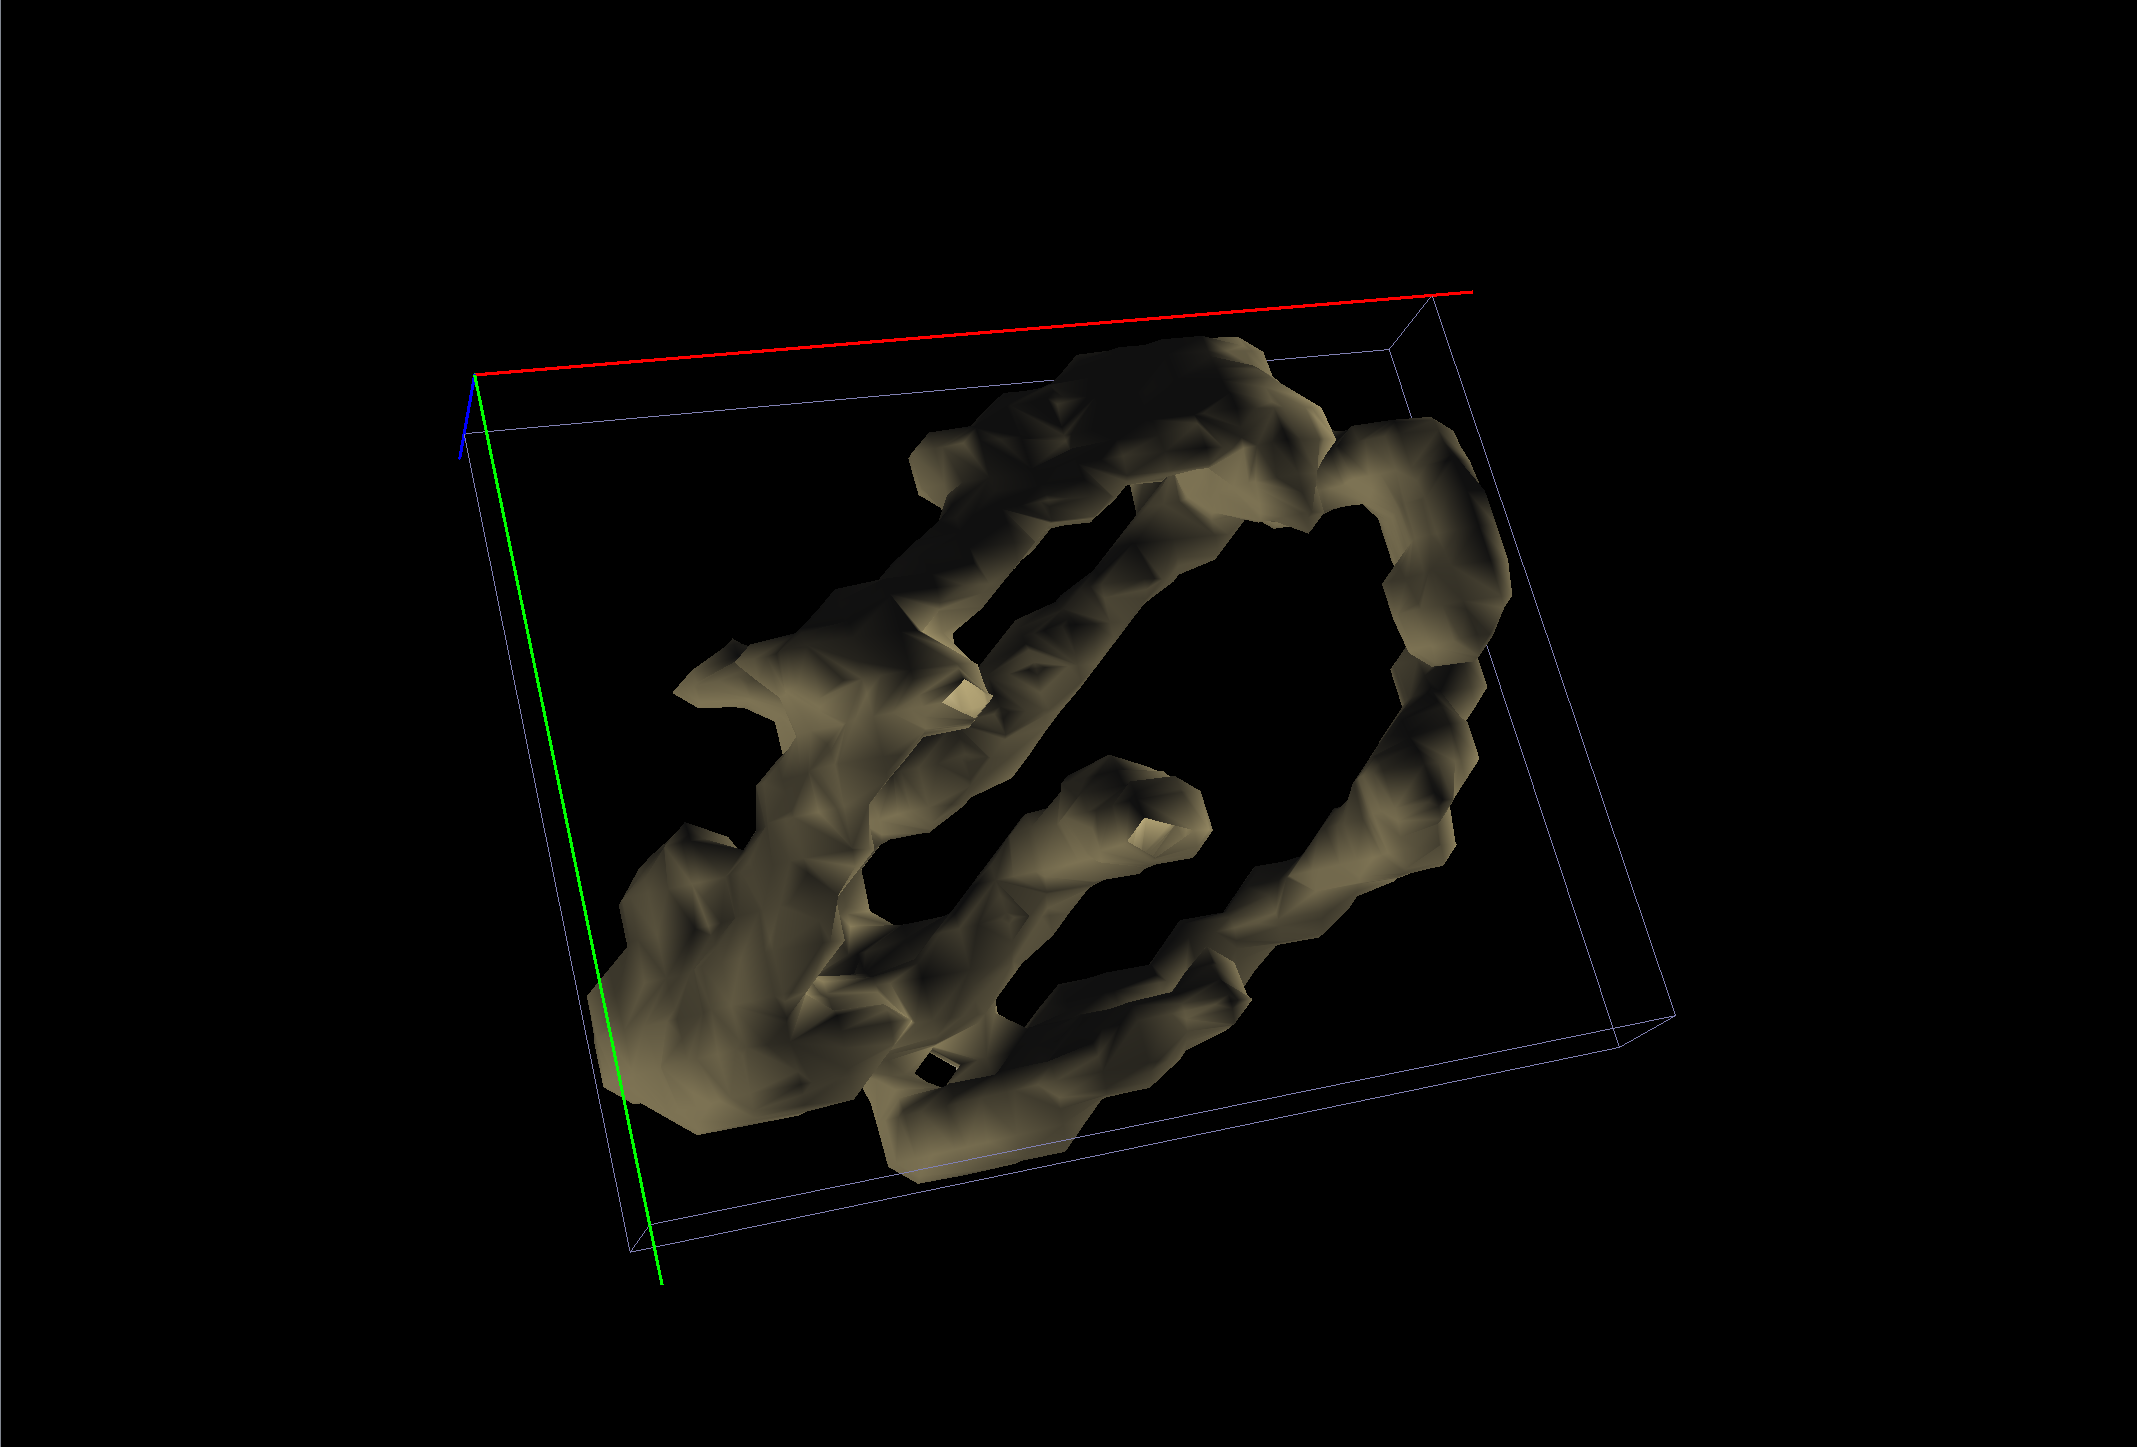
\includegraphics[width=0.3\linewidth]{Report/Images/6.3.2/0-75,25.png}
    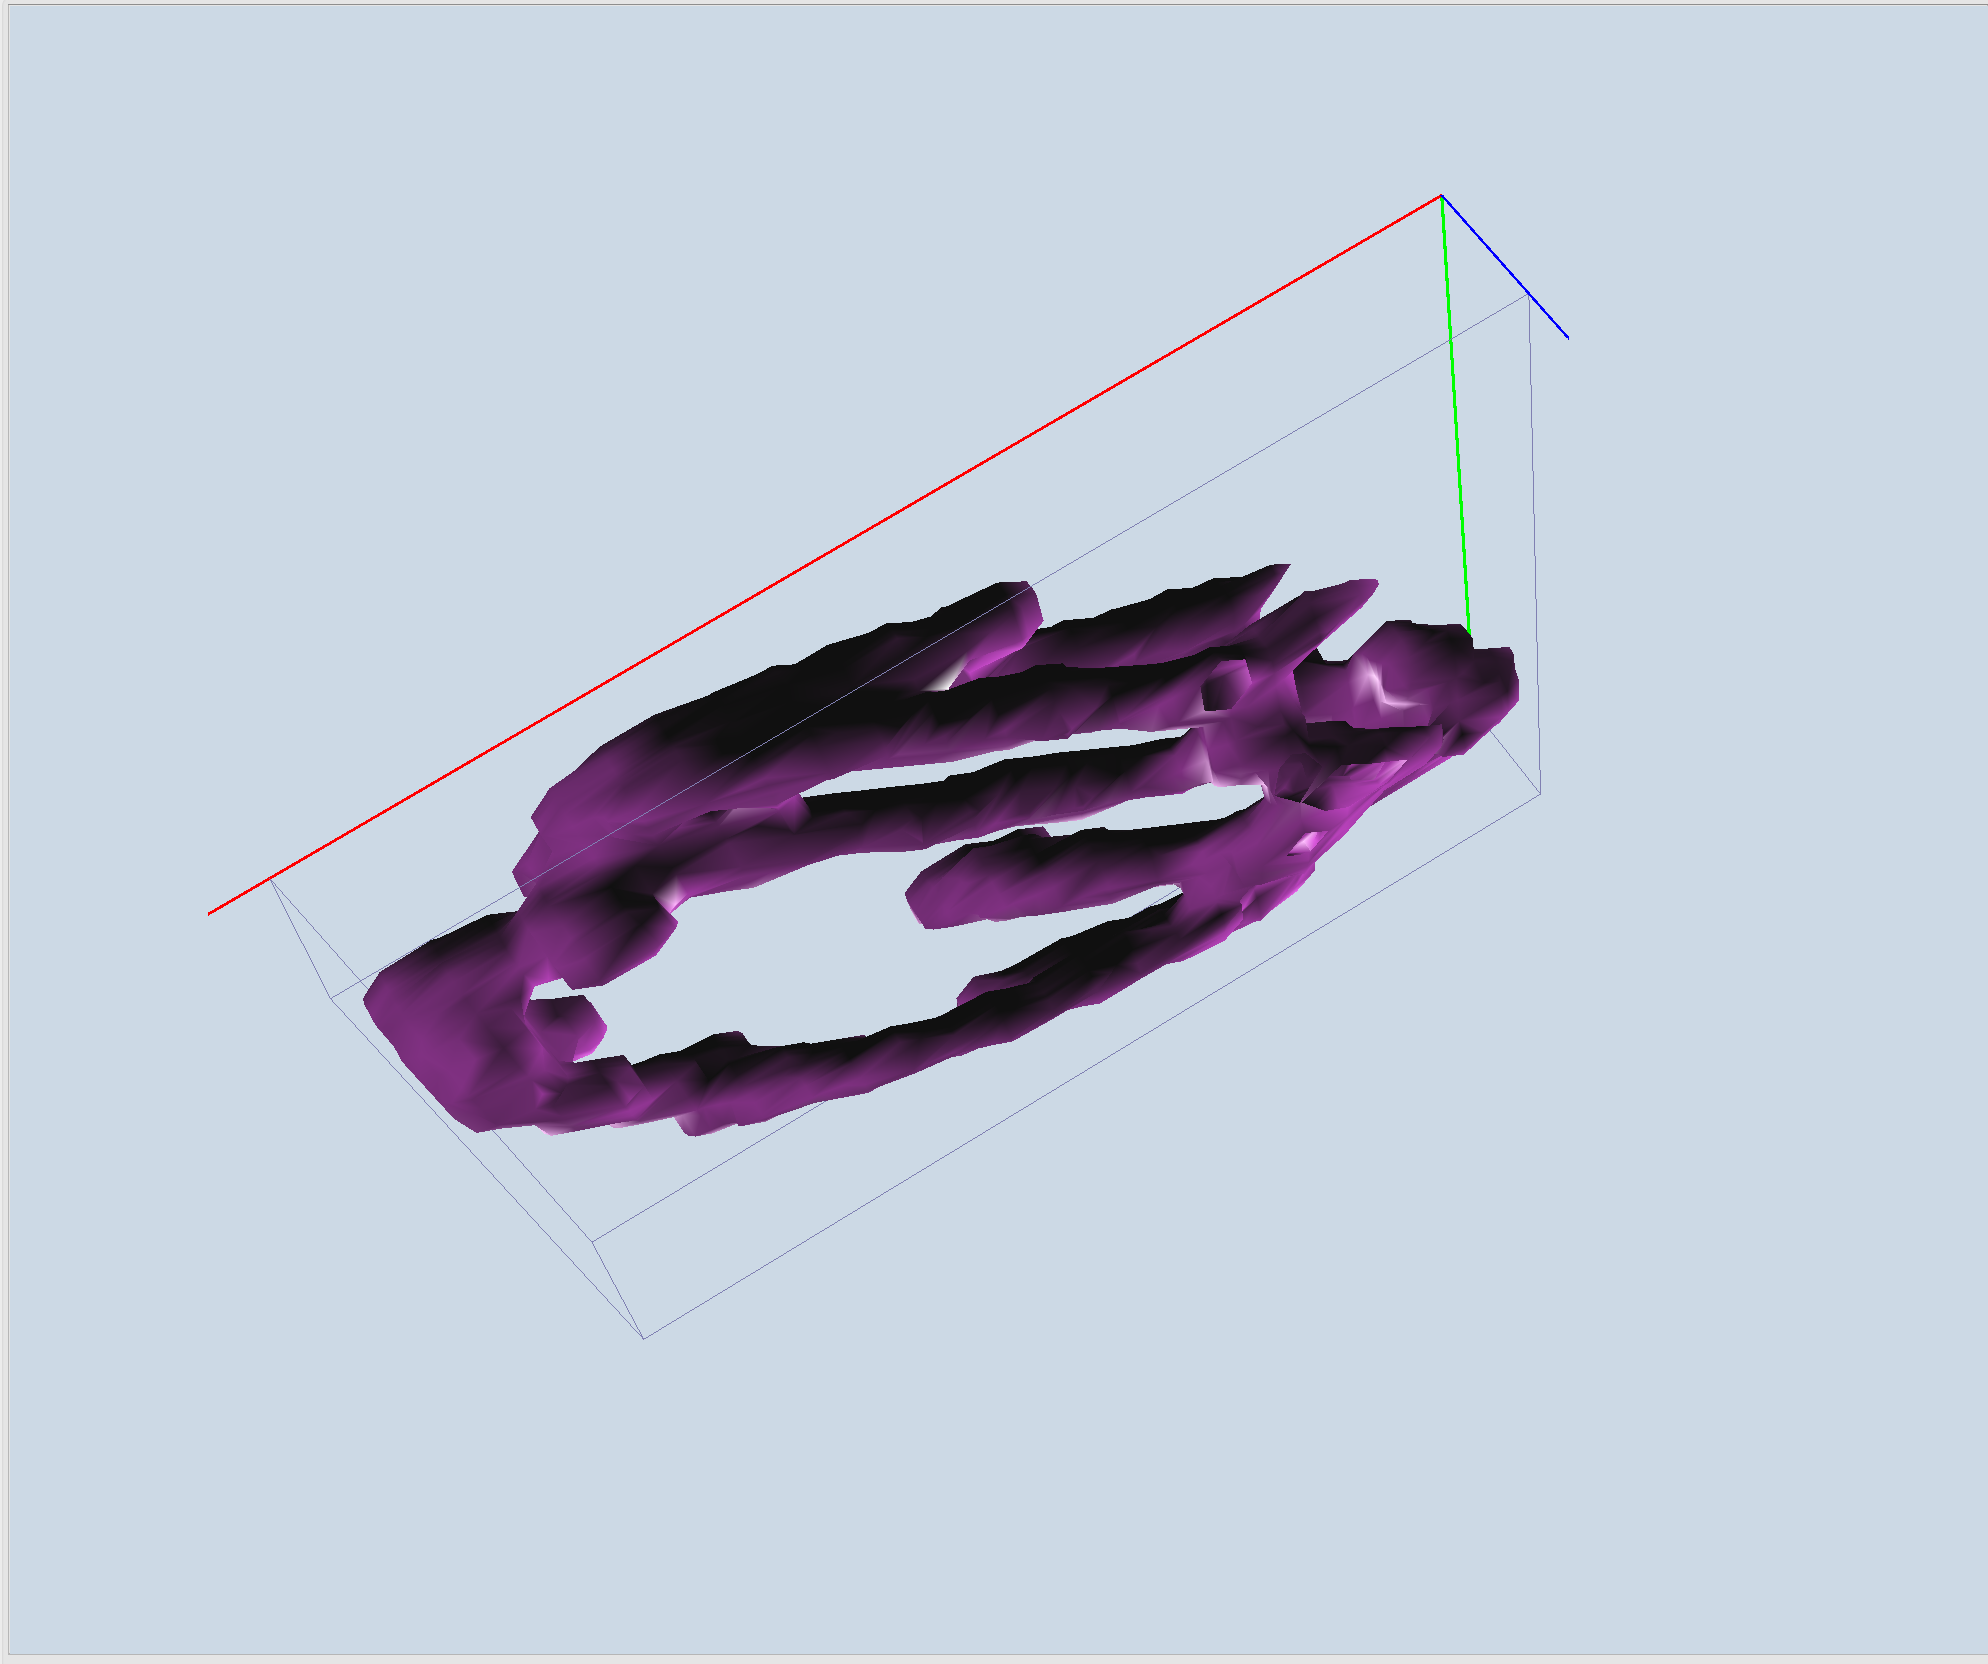
\includegraphics[width=0.3\linewidth]{Report/Images/6.3.2/0-75,25-rotated.png}
    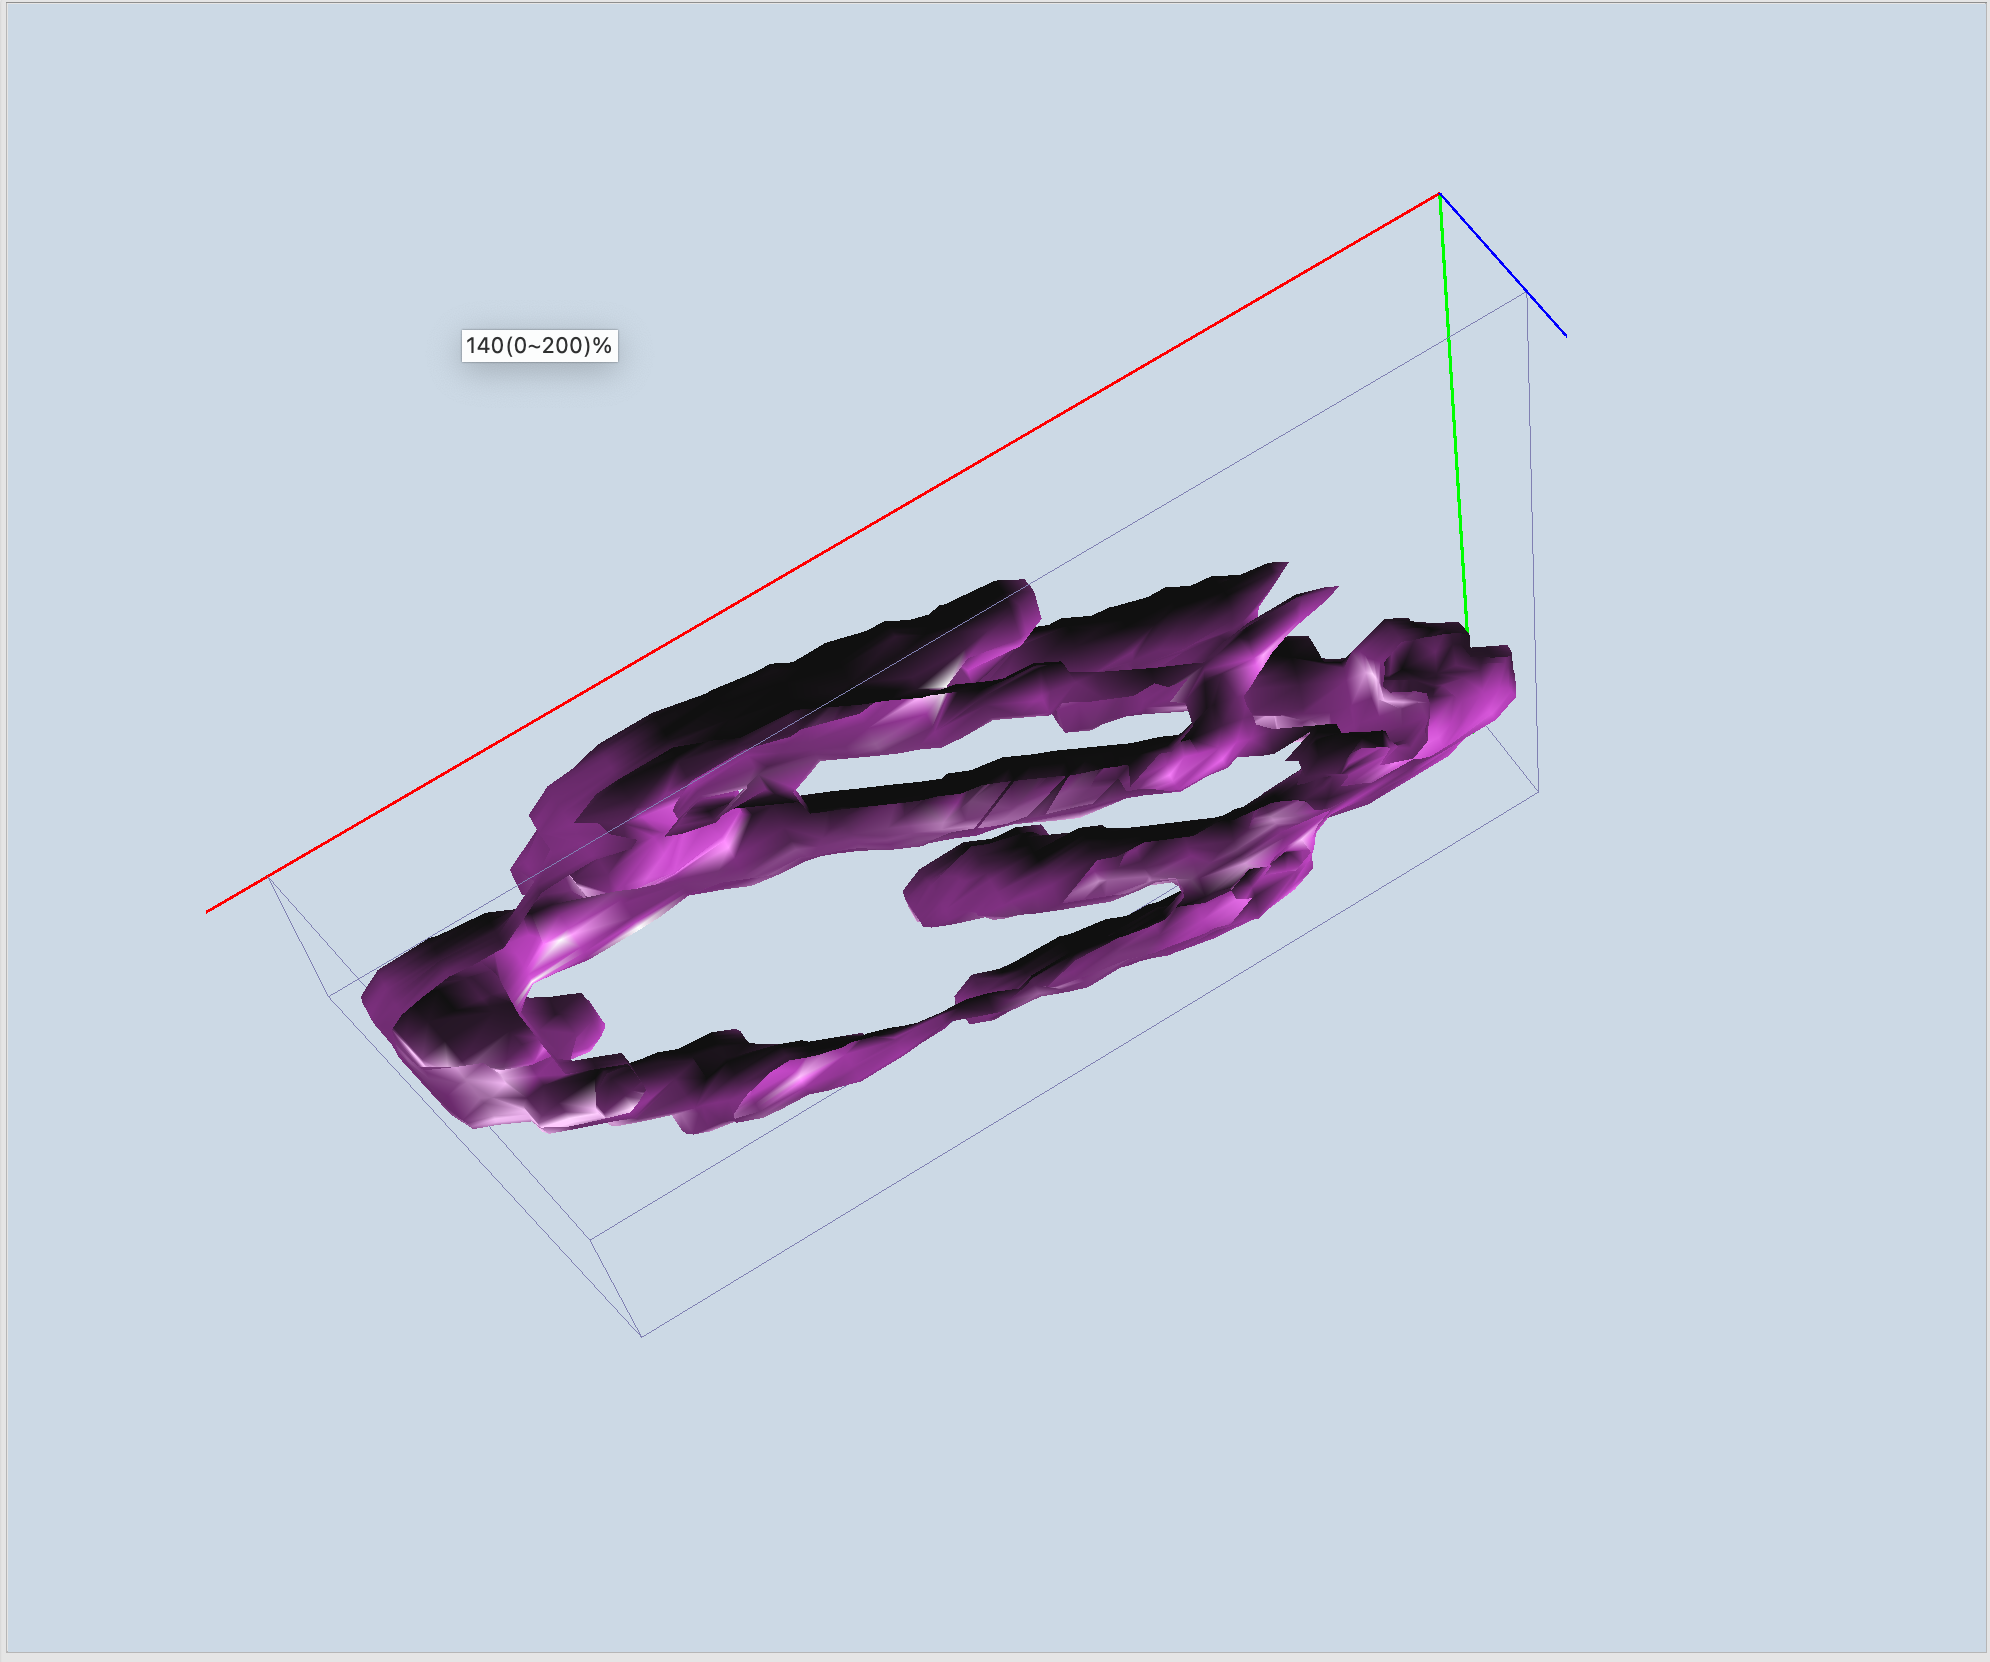
\includegraphics[width=0.3\linewidth]{Report/Images/6.3.2/0-75,25-sliced.png}
    \caption{Threshold: 0-75, mesh density:25, original (left), rotated (middle), cross-section(right)}
    \label{fig:surface_vis_0_75-25}
\end{figure}

\begin{figure}[h!]
    \centering
    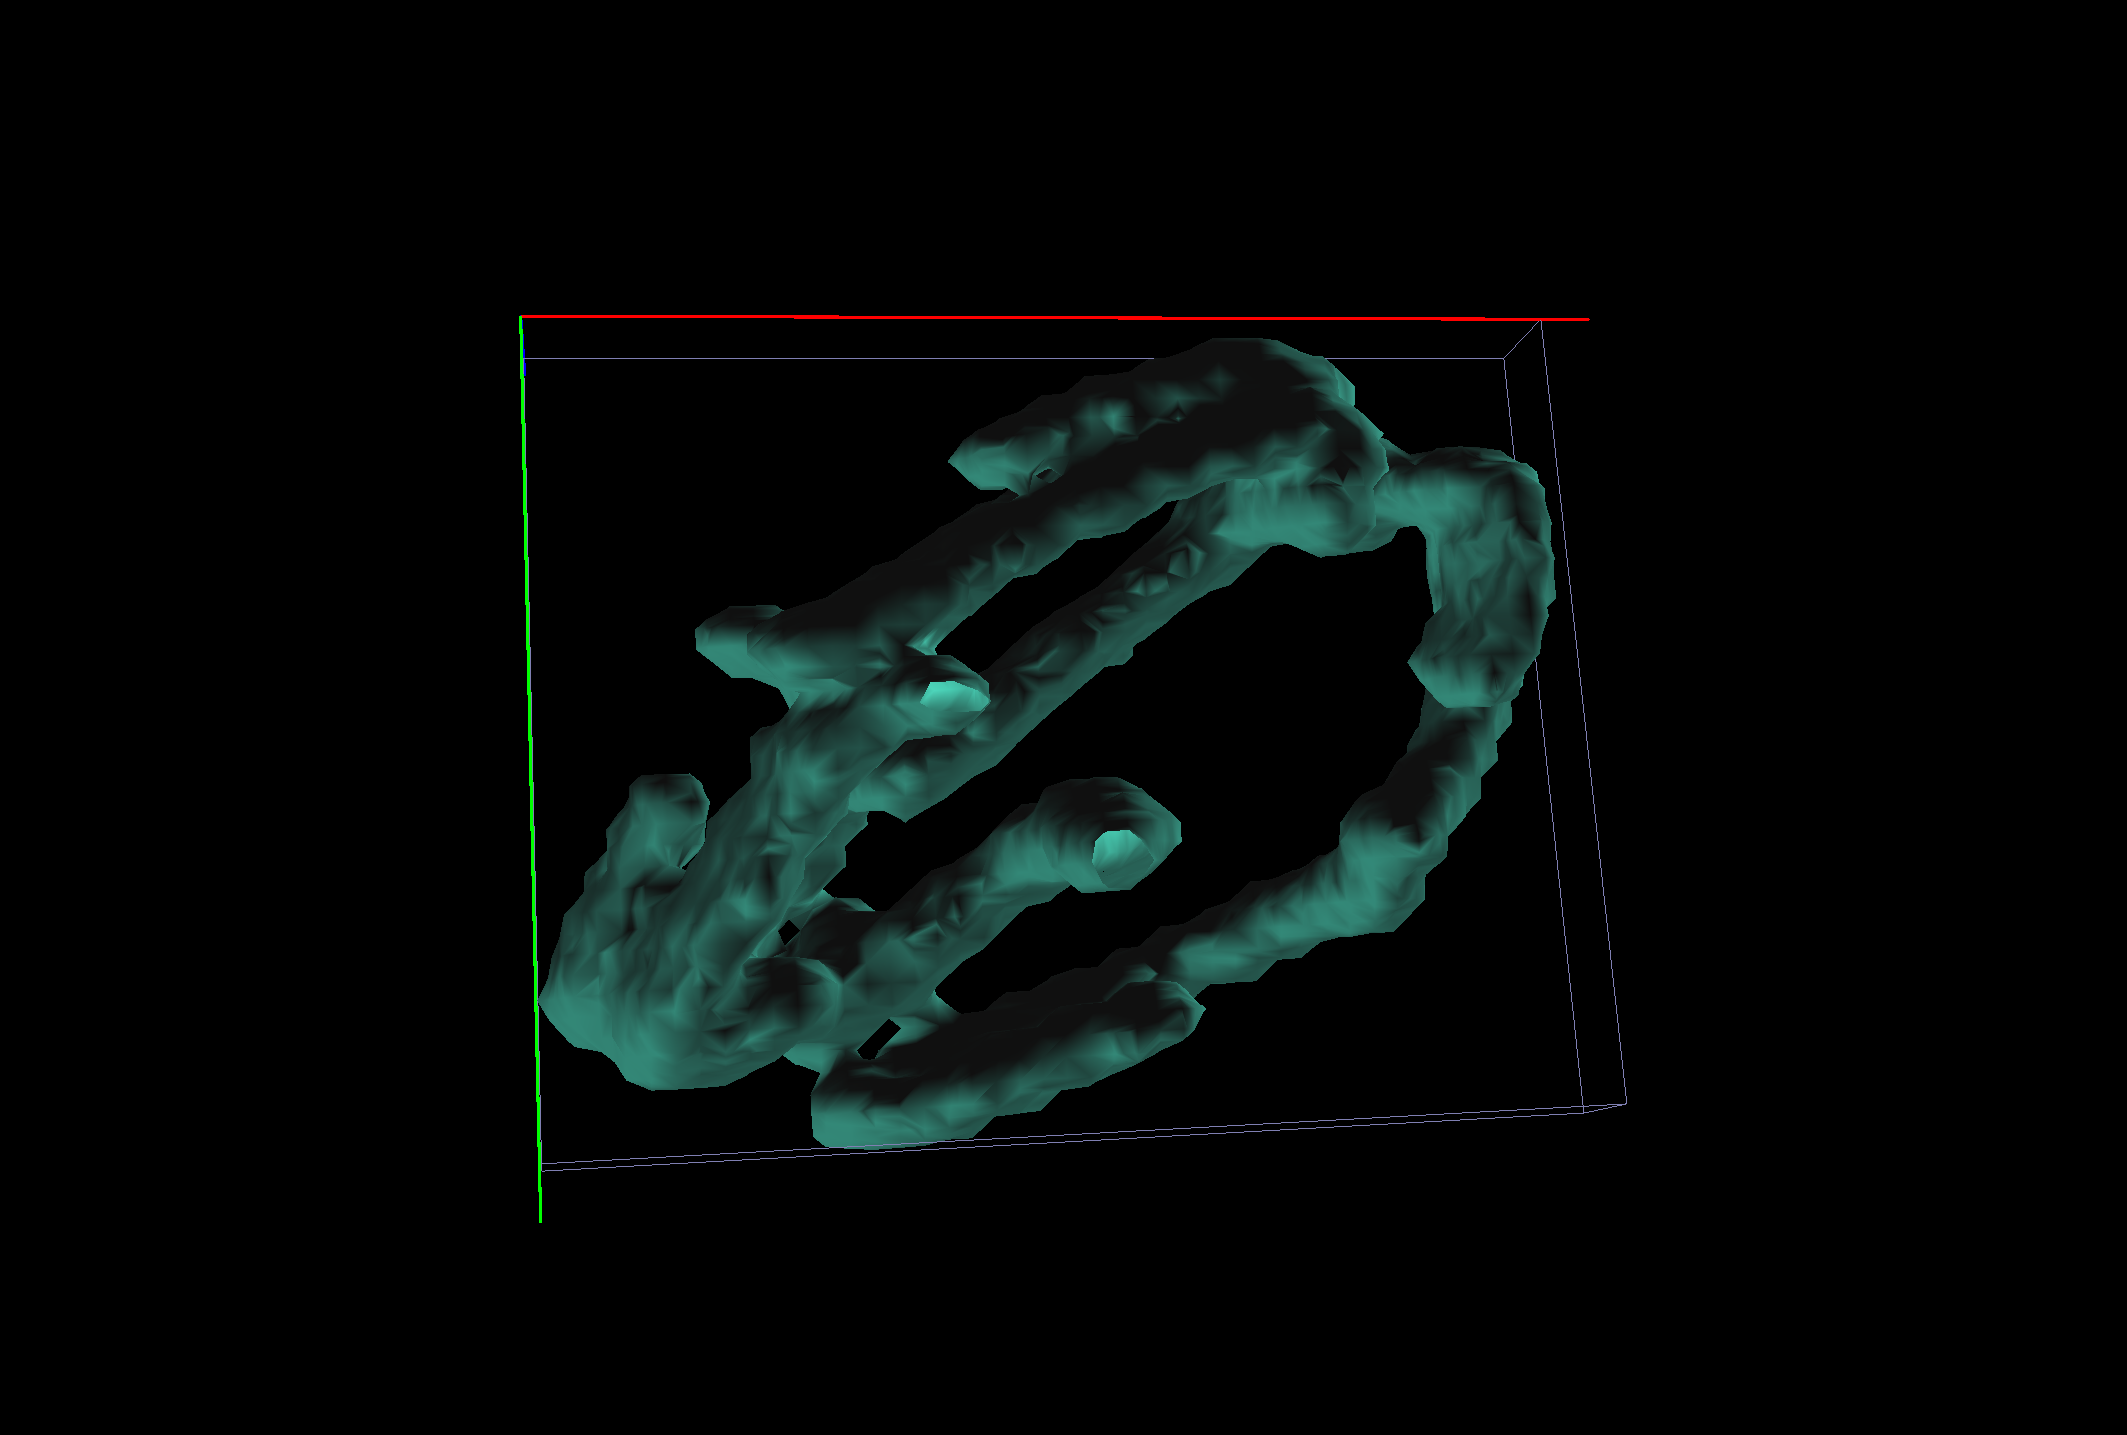
\includegraphics[width=0.3\linewidth]{Report/Images/6.3.2/0-75,50.png}
    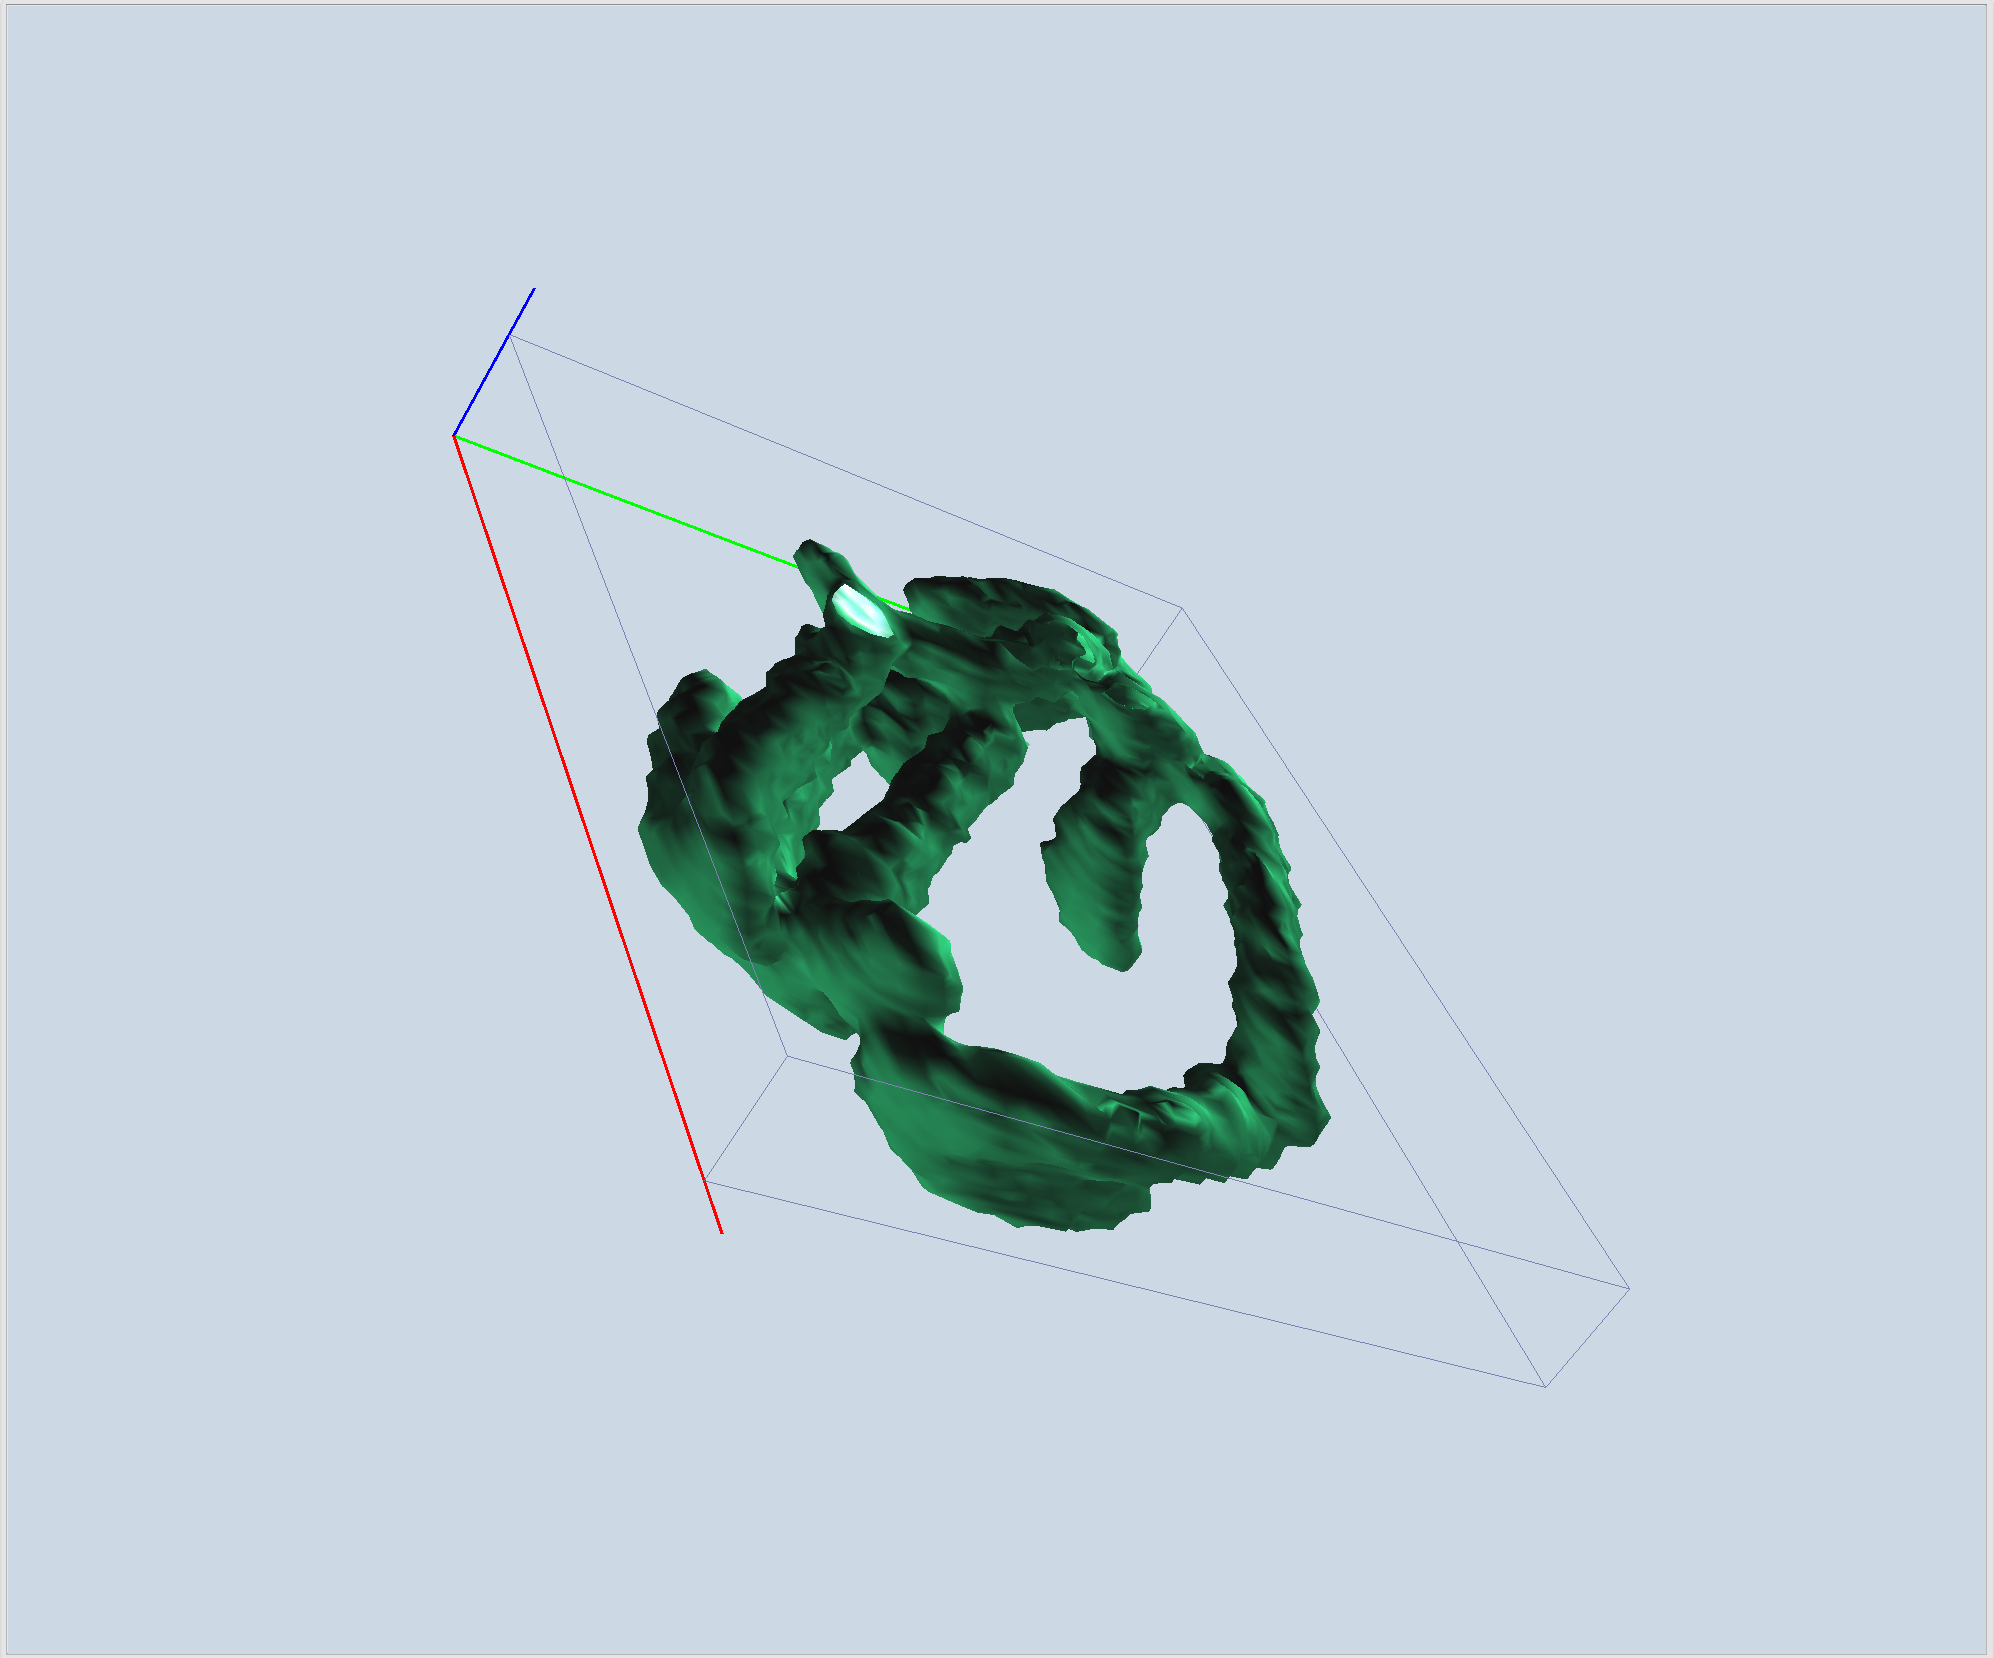
\includegraphics[width=0.3\linewidth]{Report/Images/6.3.2/0-75,50-rotated.png}
    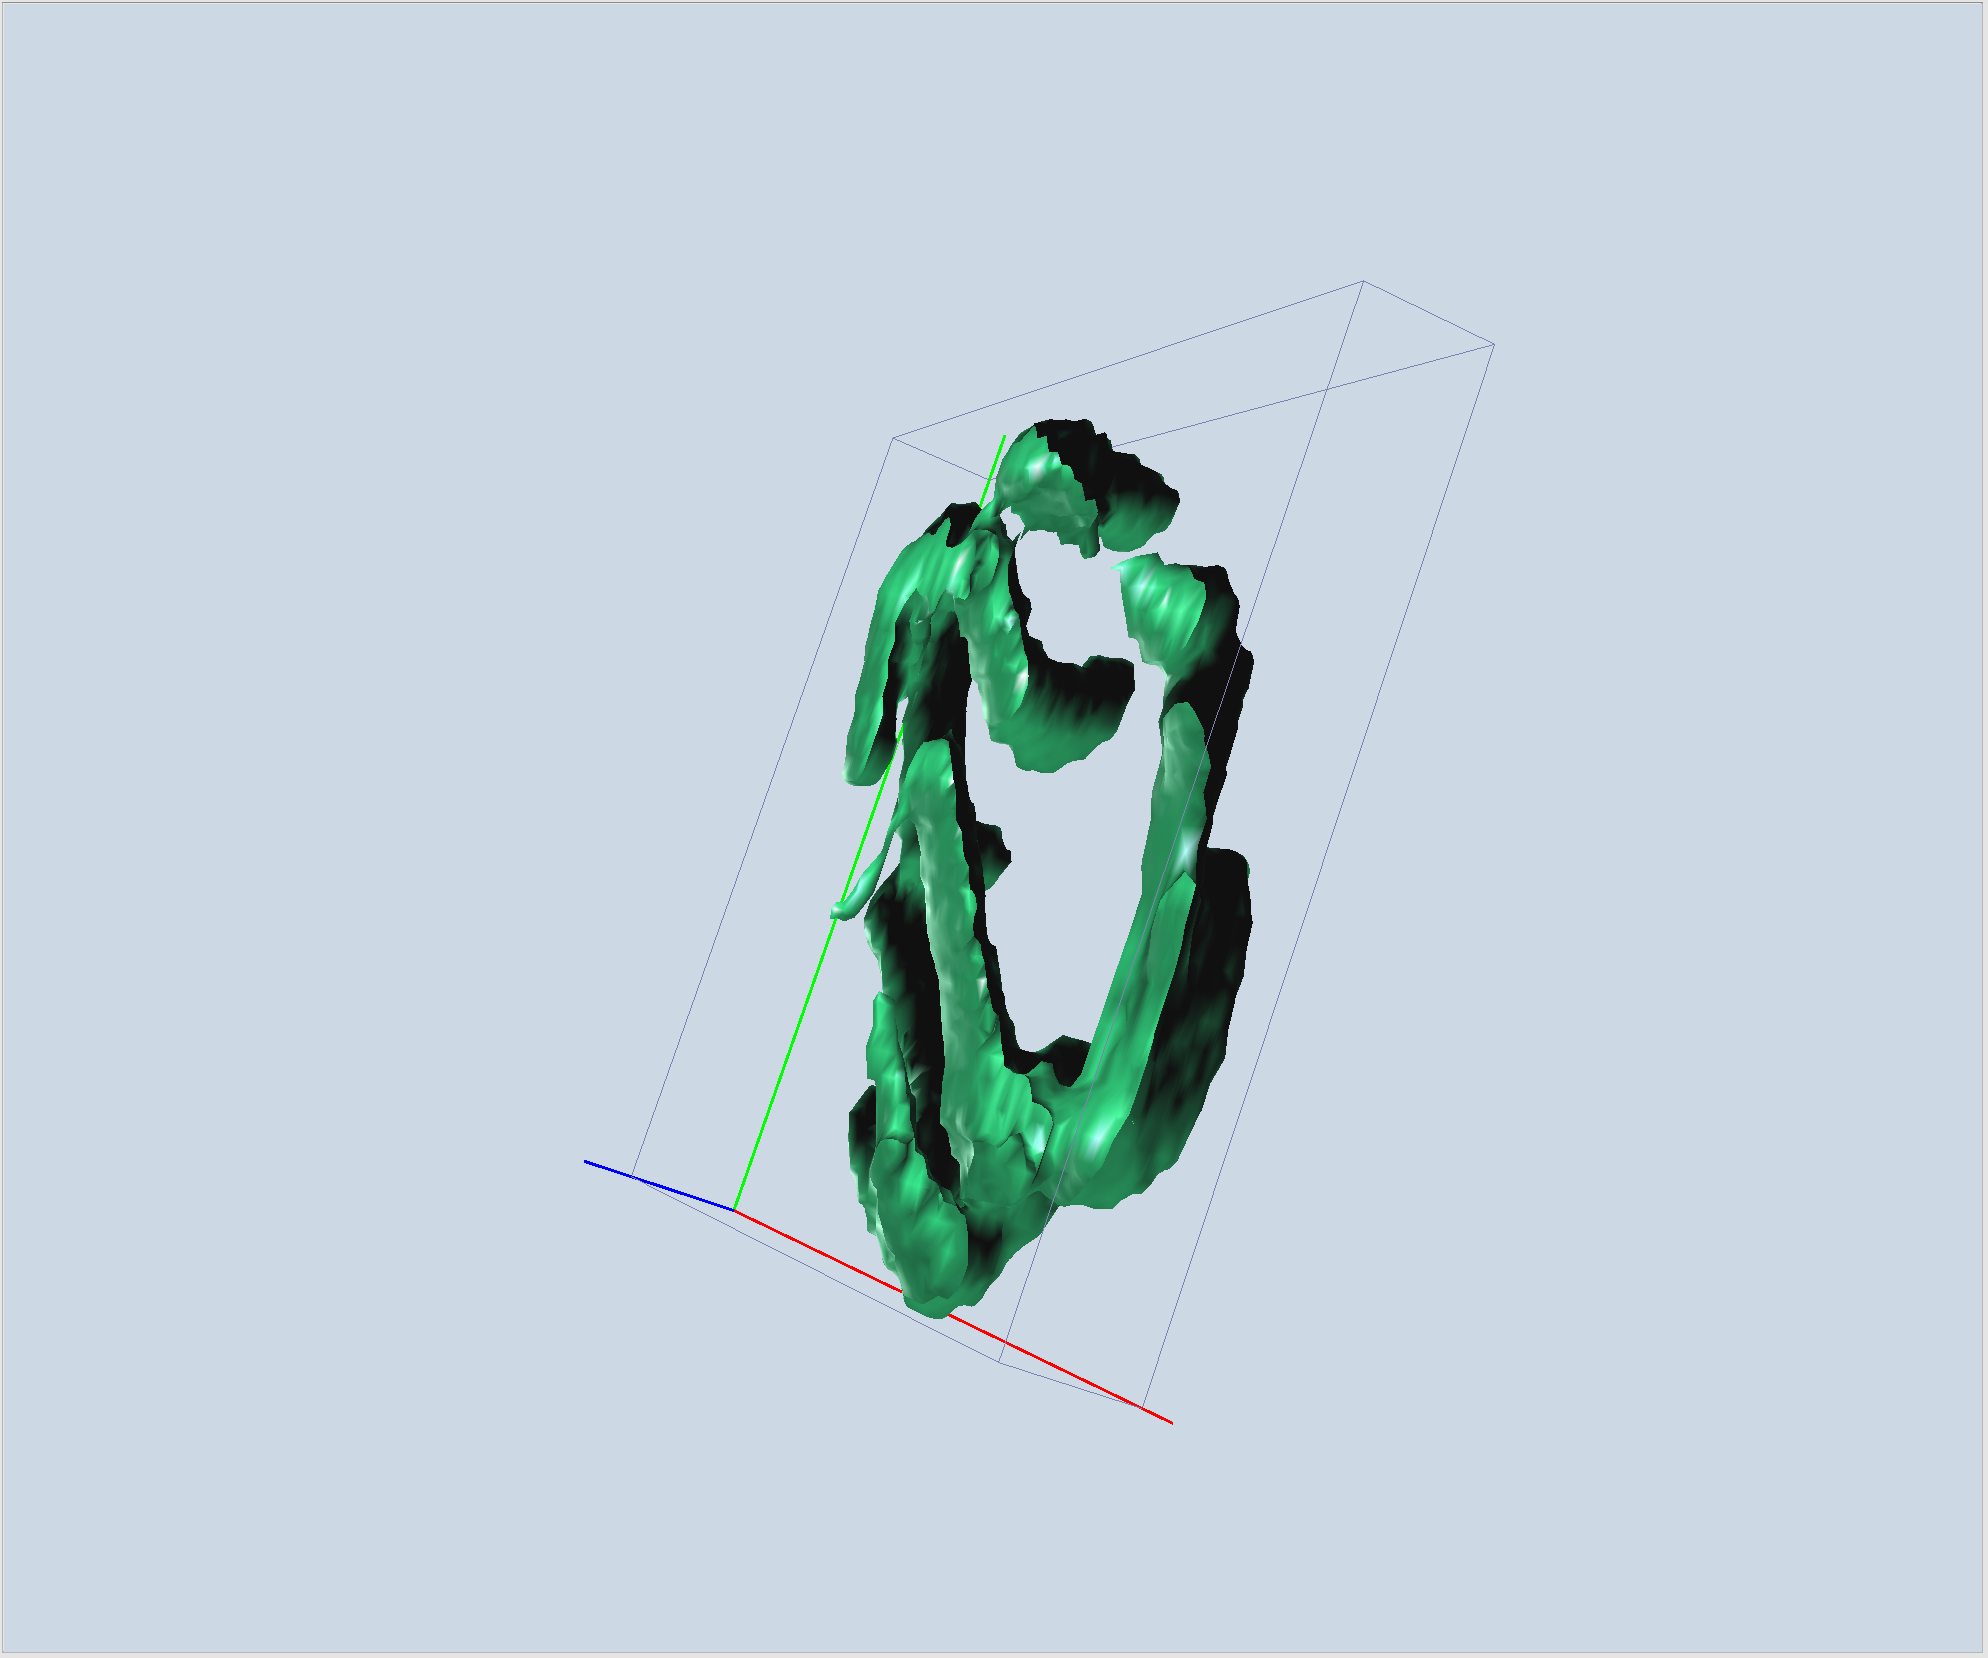
\includegraphics[width=0.3\linewidth]{Report/Images/6.3.2/0-75,50-sliced.png}
    \caption{Threshold: 0-75, mesh density:50, original (left), rotated (middle), cross-section(right)}
    \label{fig:surface_vis_0_75-50}
\end{figure}


\begin{figure}[h!]
    \centering
    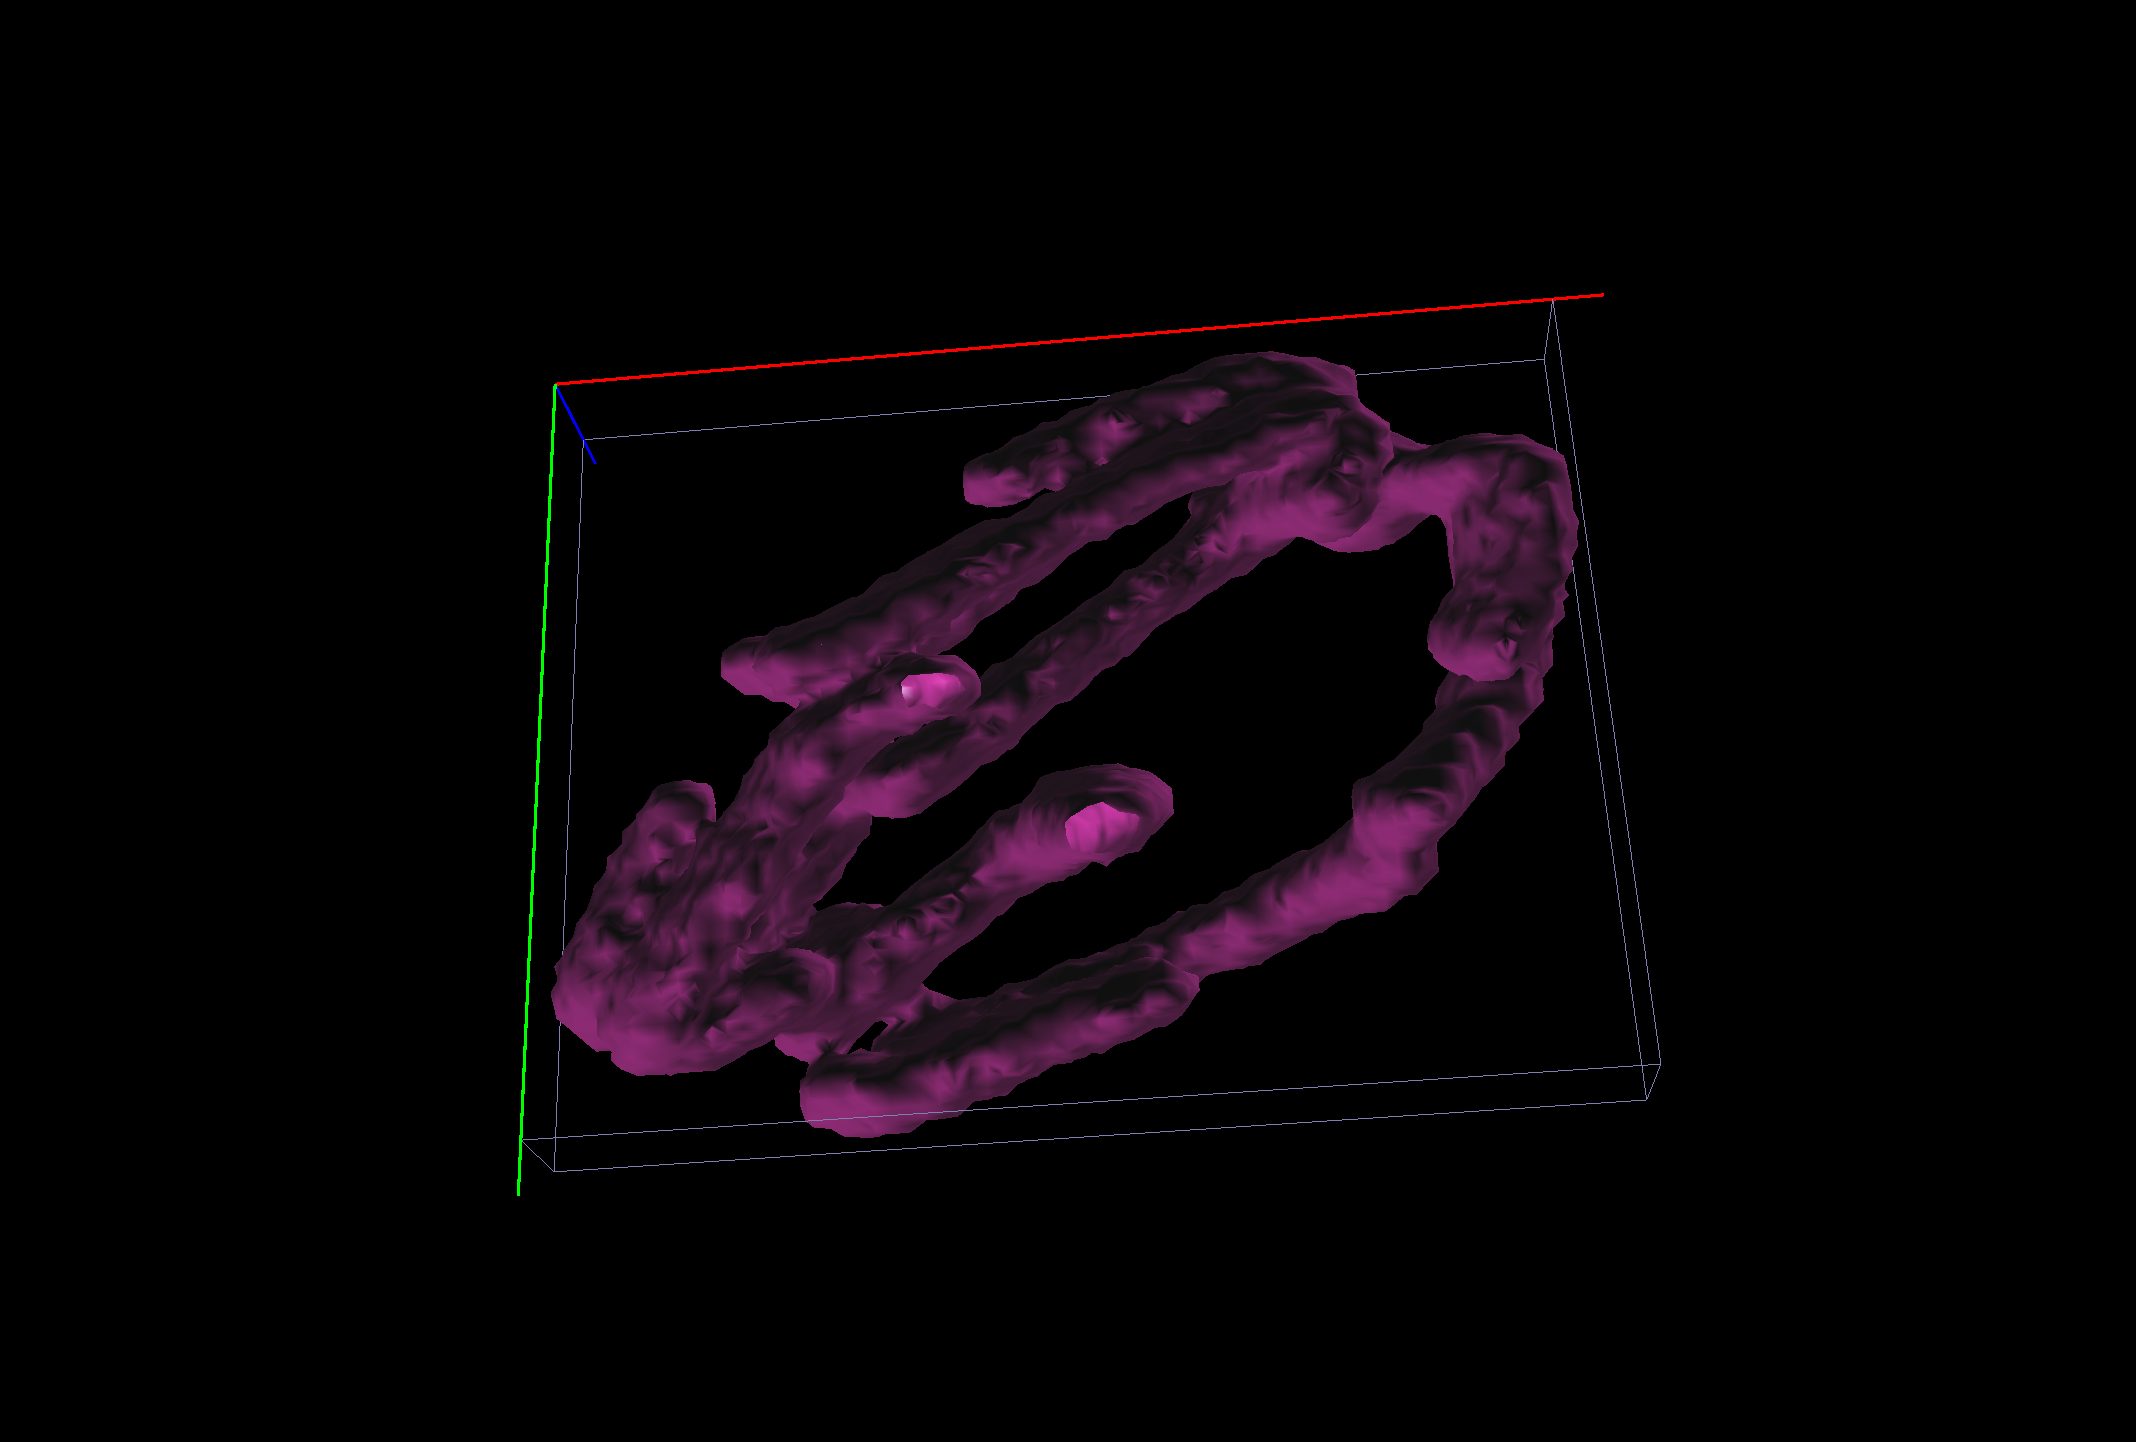
\includegraphics[width=0.3\linewidth]{Report/Images/6.3.2/0-75,75.png}
    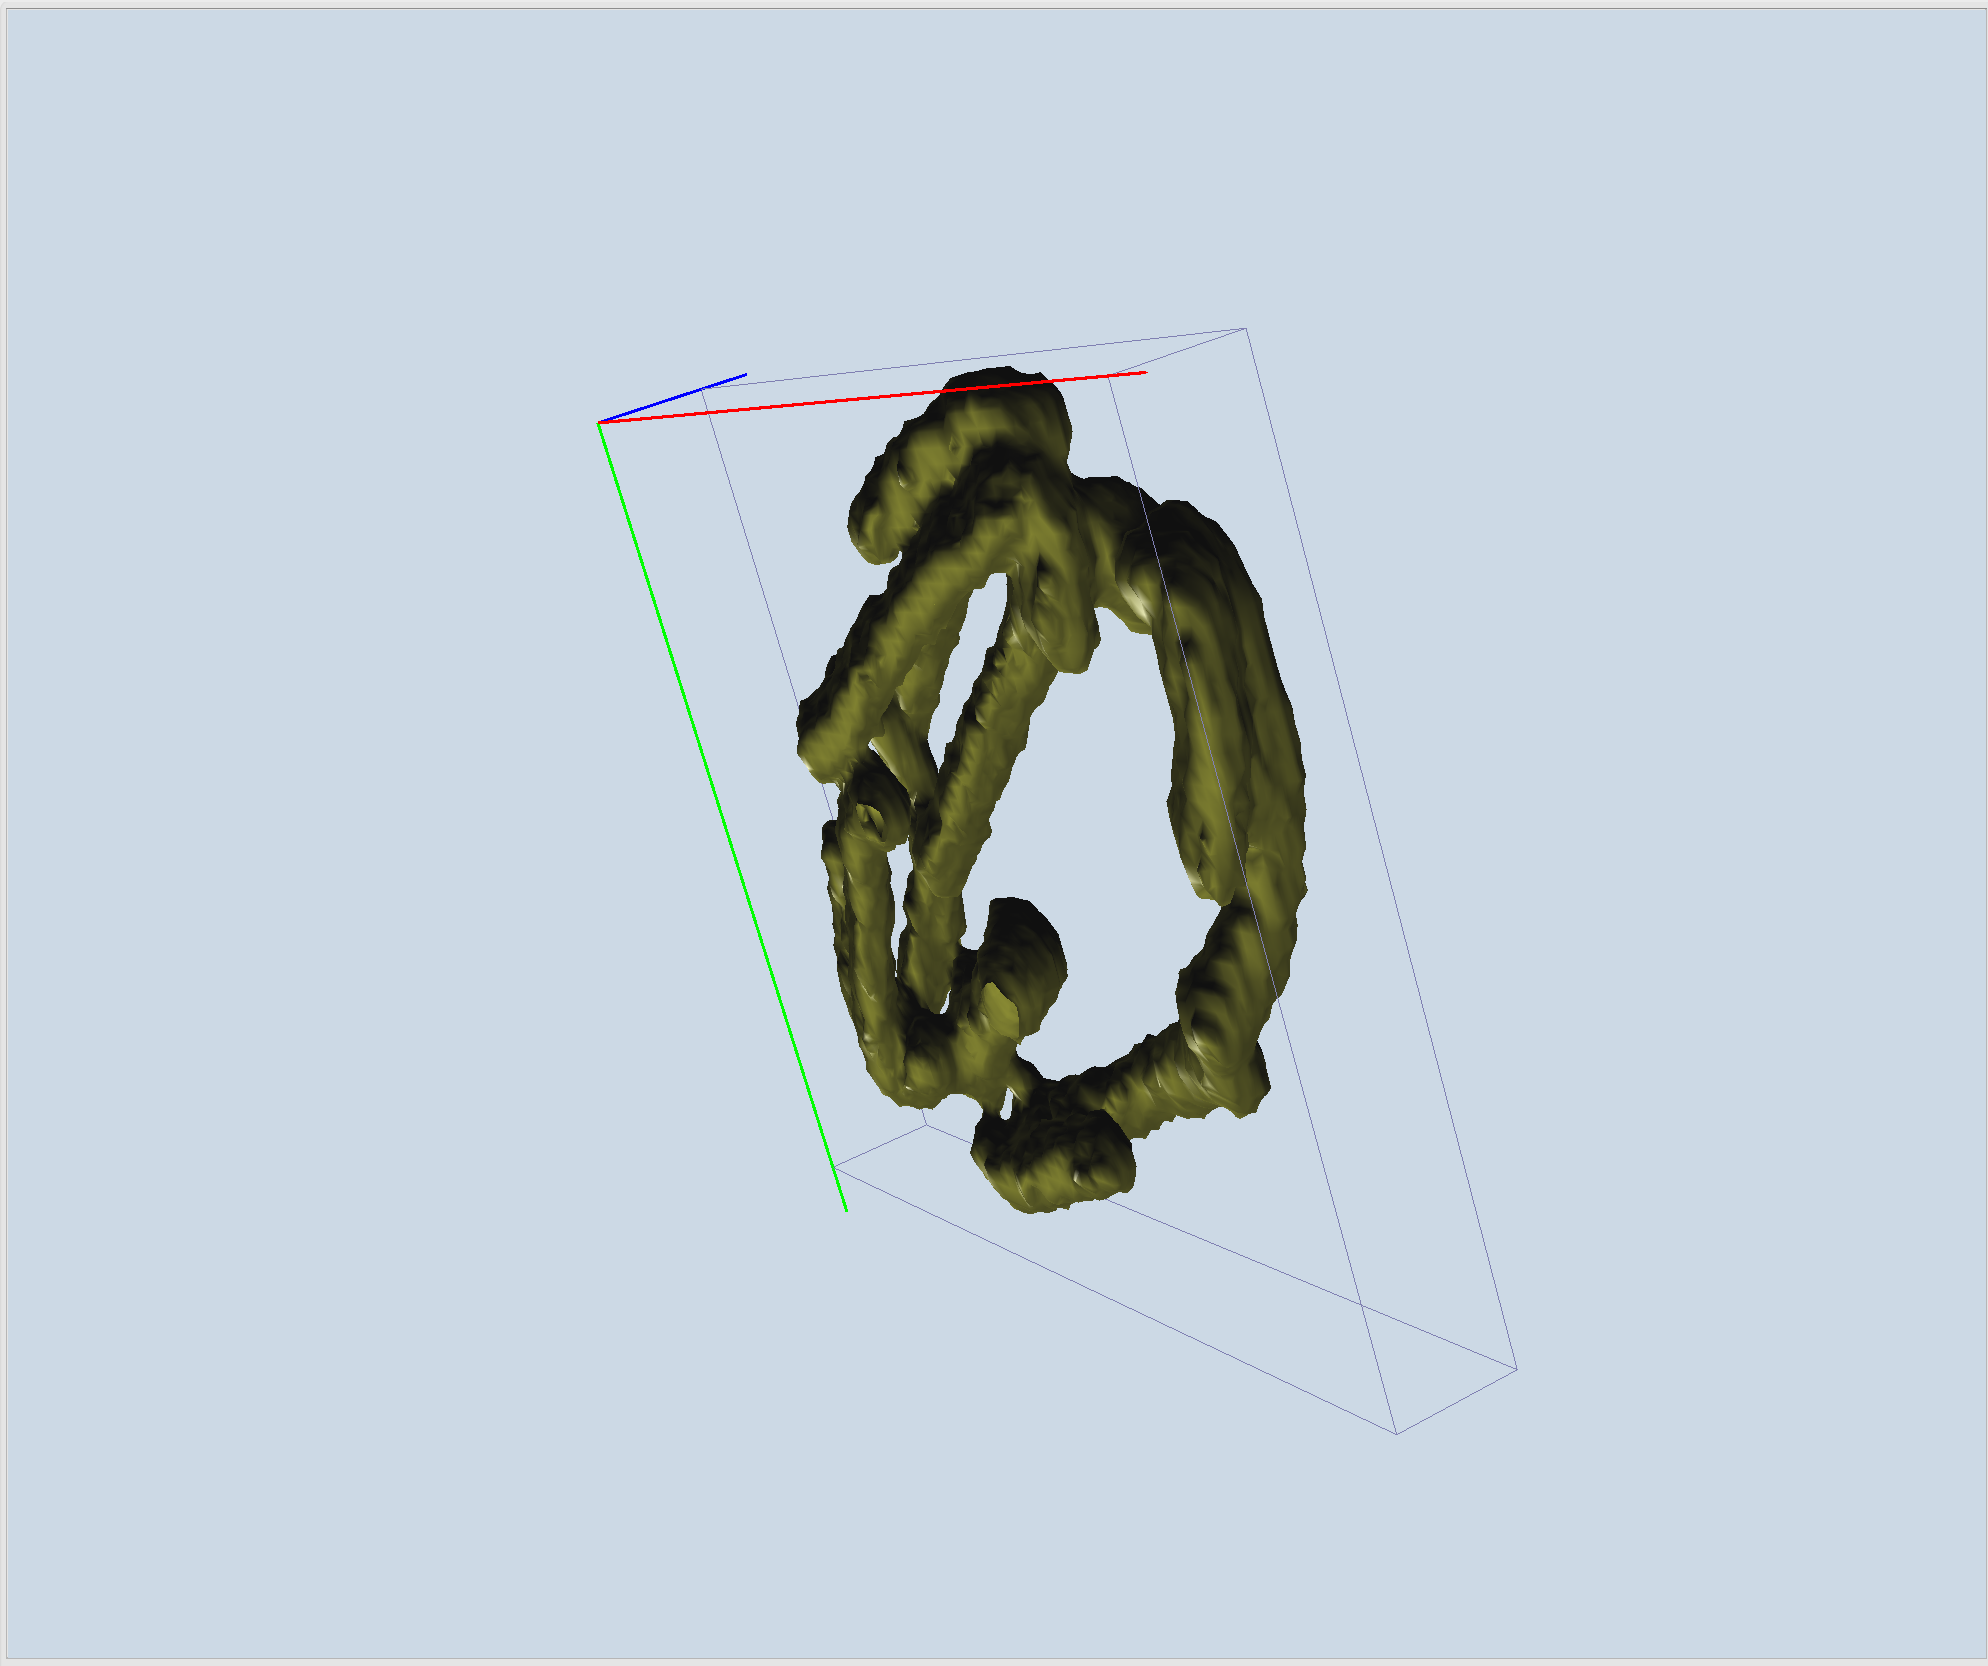
\includegraphics[width=0.3\linewidth]{Report/Images/6.3.2/0-75,75-rotated.png}
    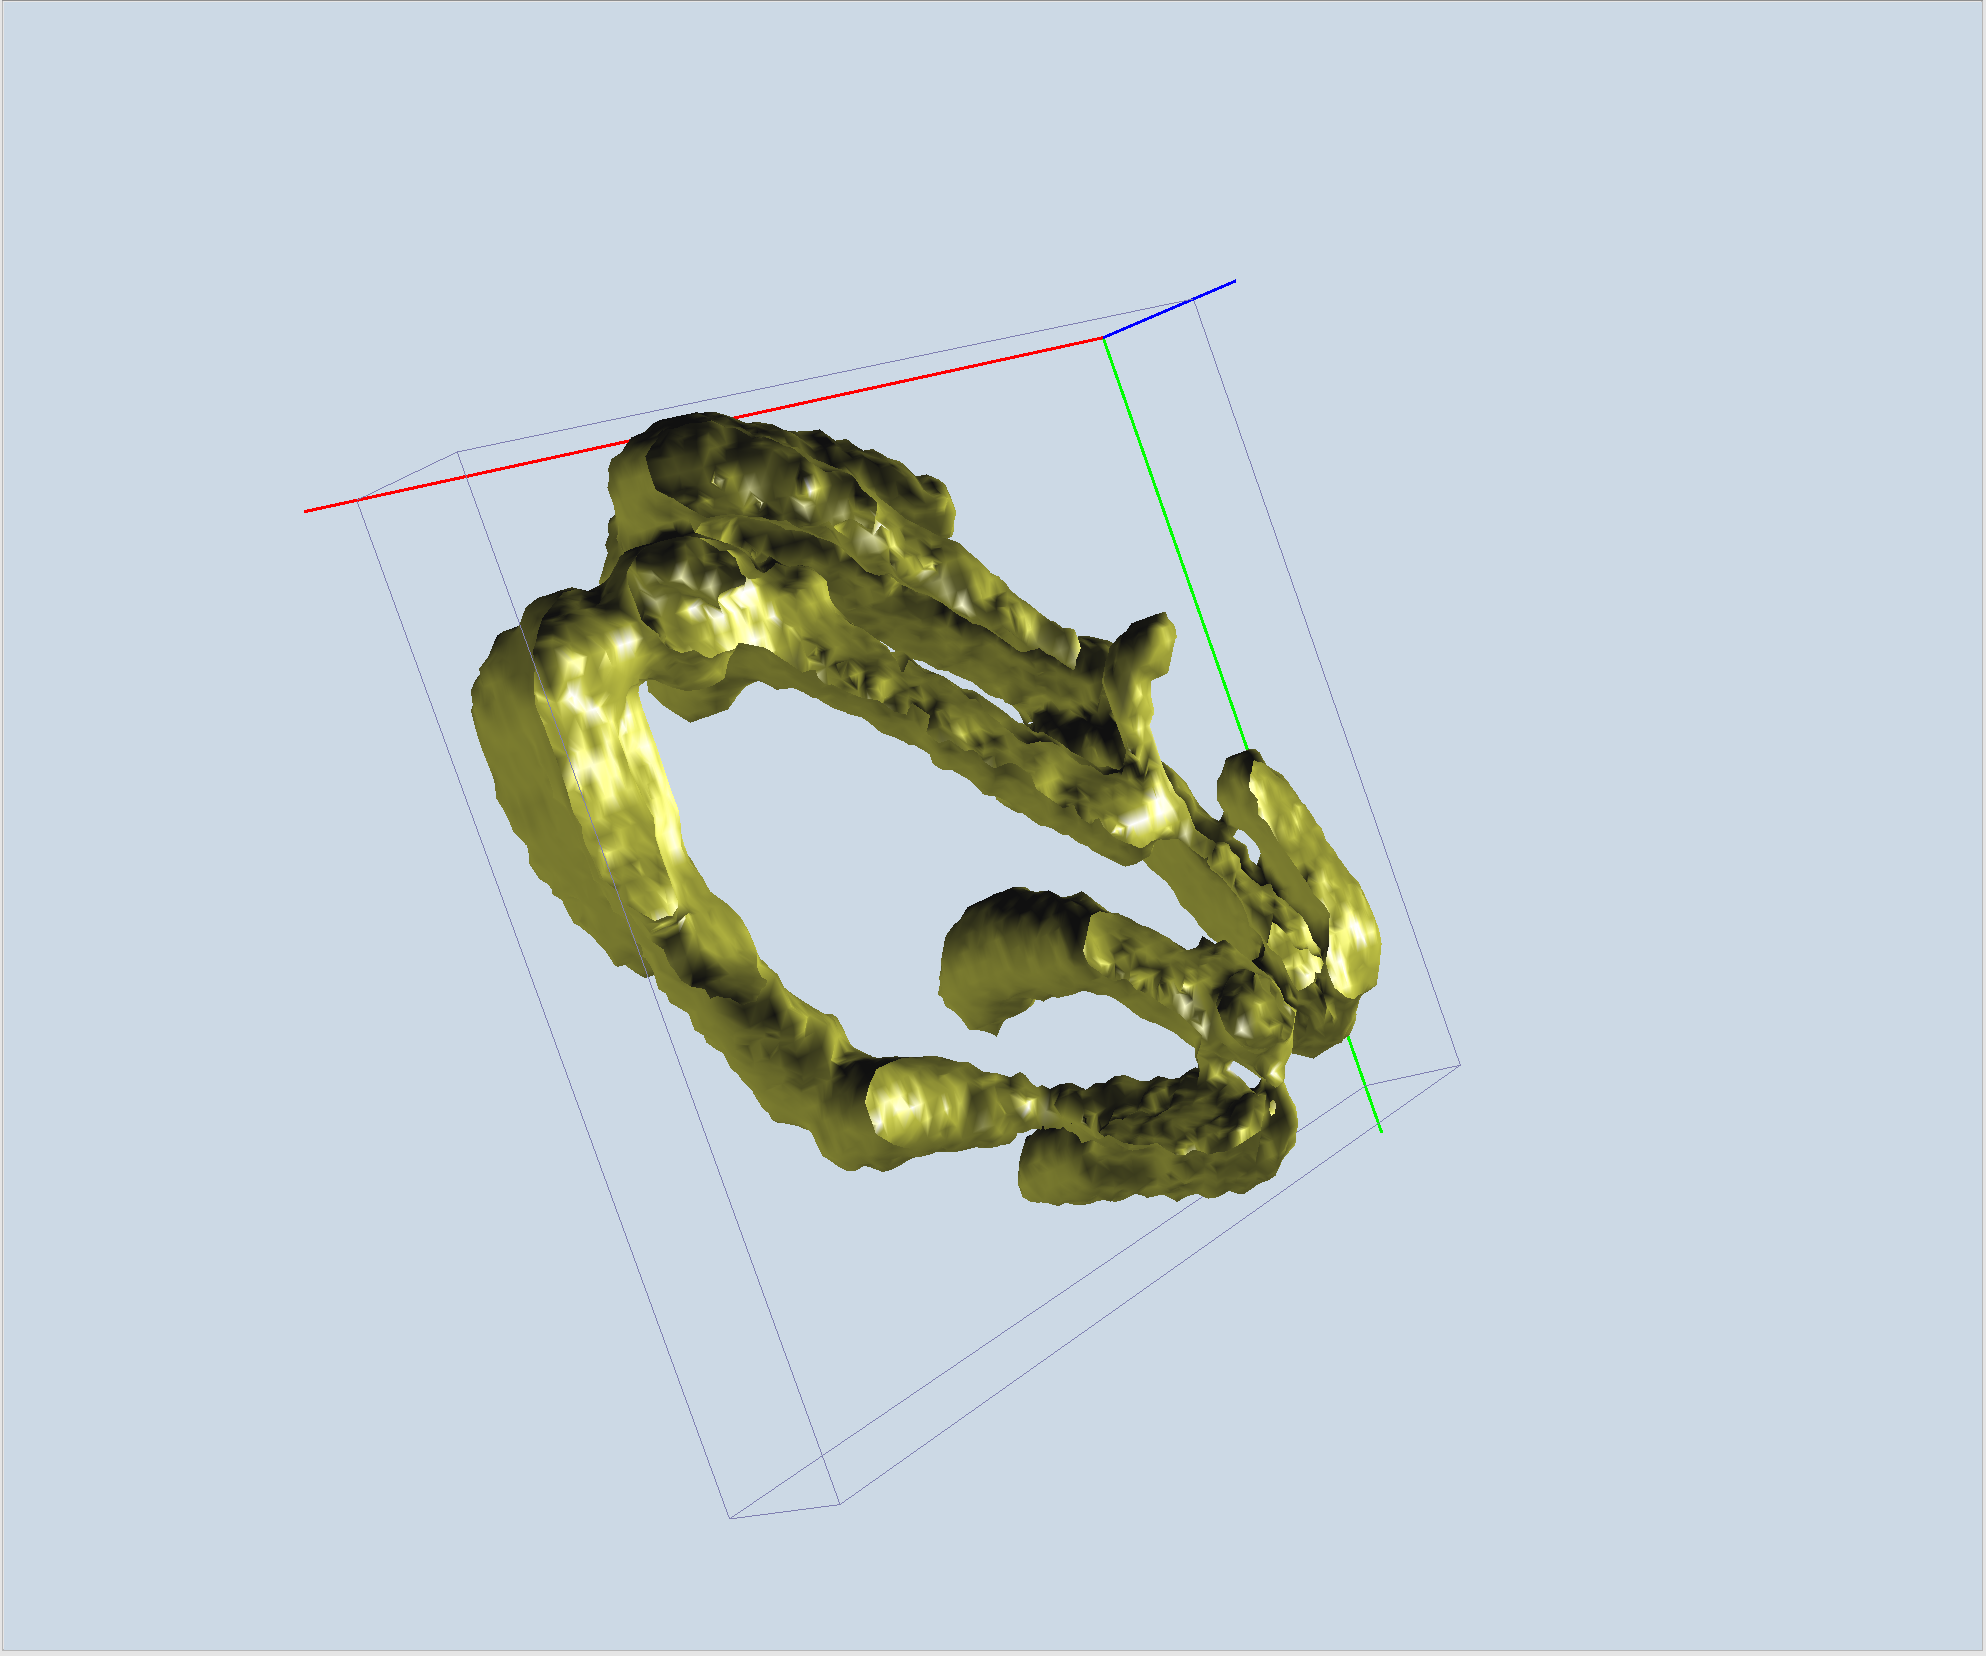
\includegraphics[width=0.3\linewidth]{Report/Images/6.3.2/0-75,75-sliced.png}
    \caption{Threshold: 0-75, mesh density:75, original (left), rotated (middle), cross-section(right)}
    \label{fig:surface_vis_0_75-75}
\end{figure}

\begin{figure}[h!]
    \centering
    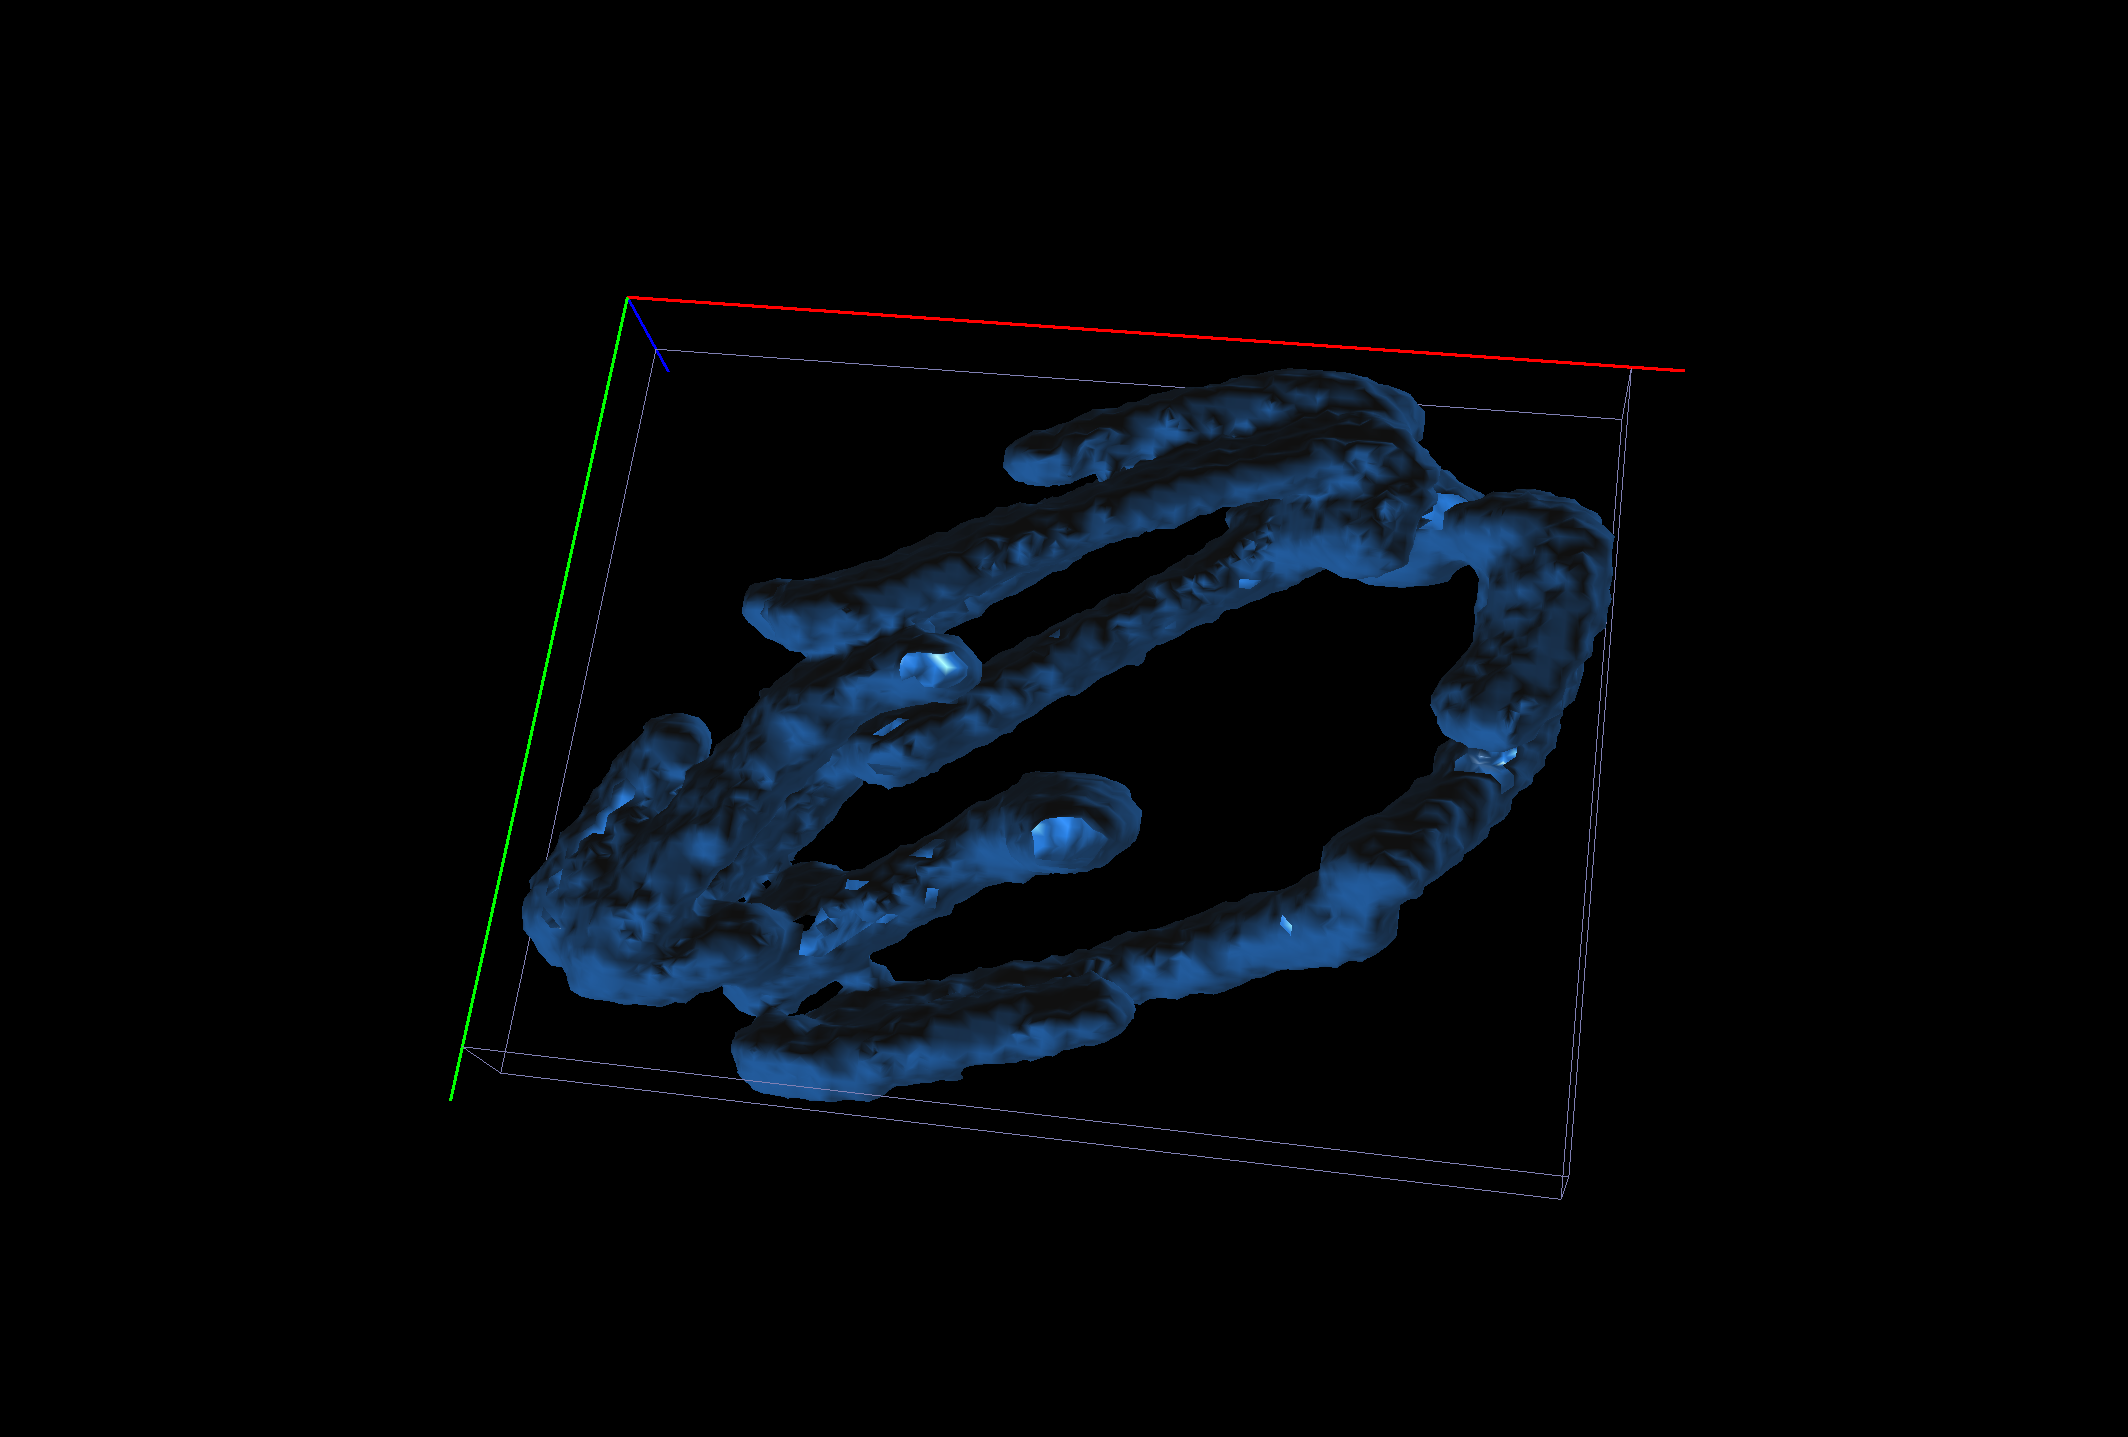
\includegraphics[width=0.3\linewidth]{Report/Images/6.3.2/0-75,100.png}
    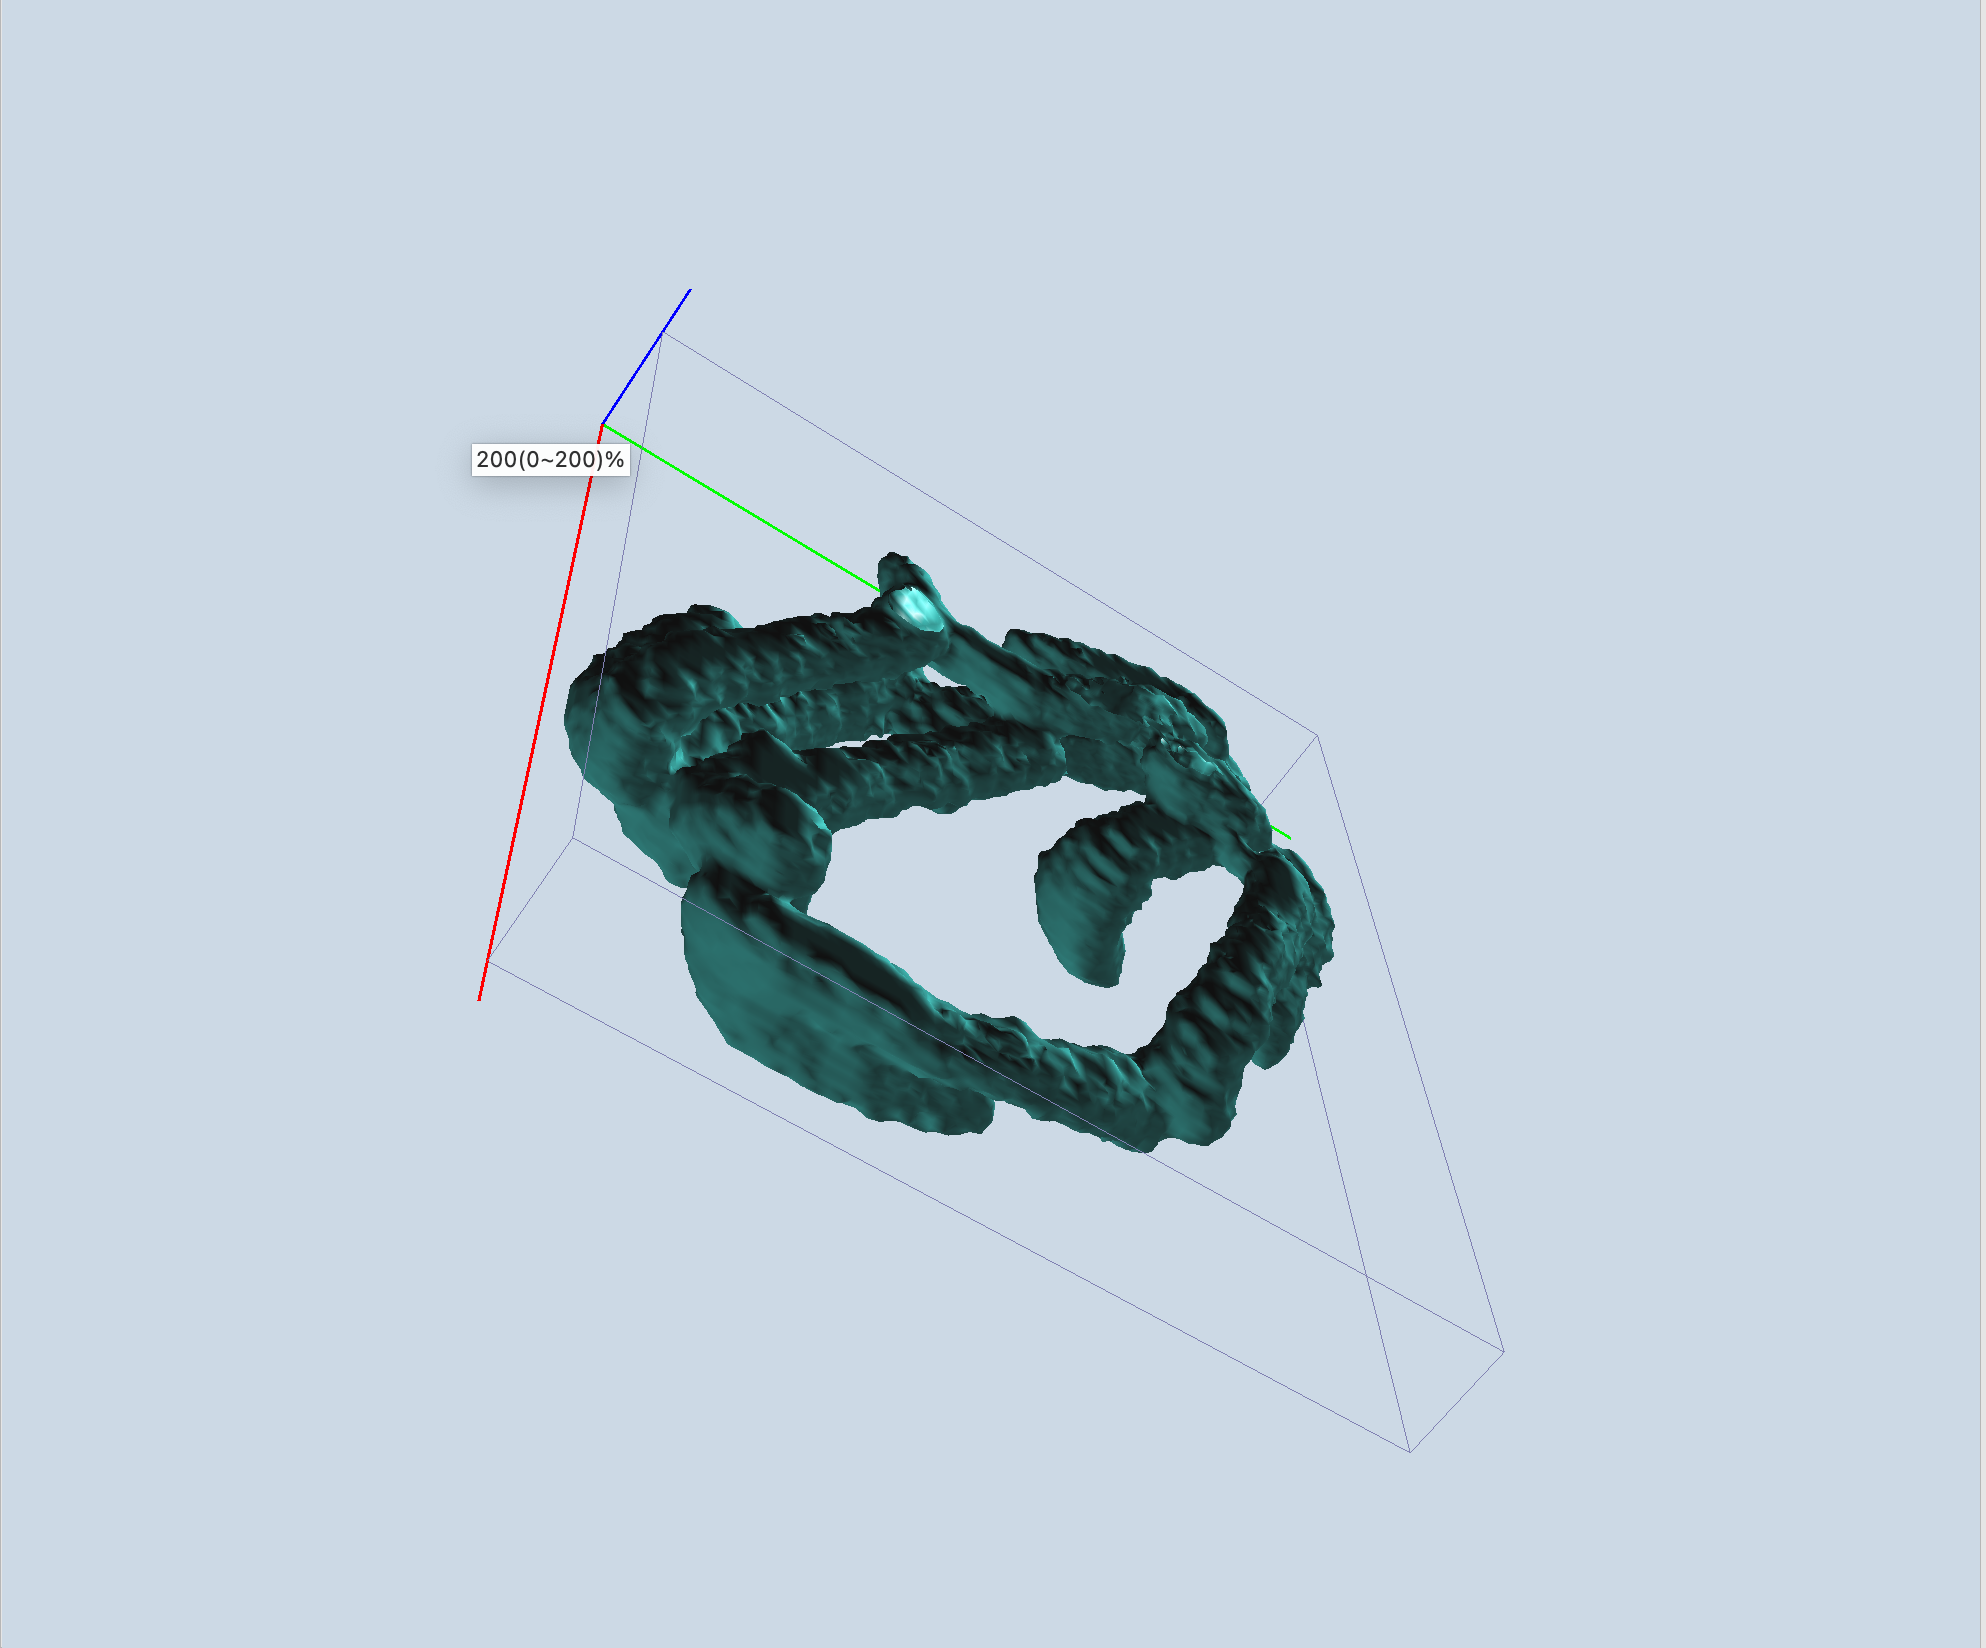
\includegraphics[width=0.3\linewidth]{Report/Images/6.3.2/0-75,100-rotated.png}
    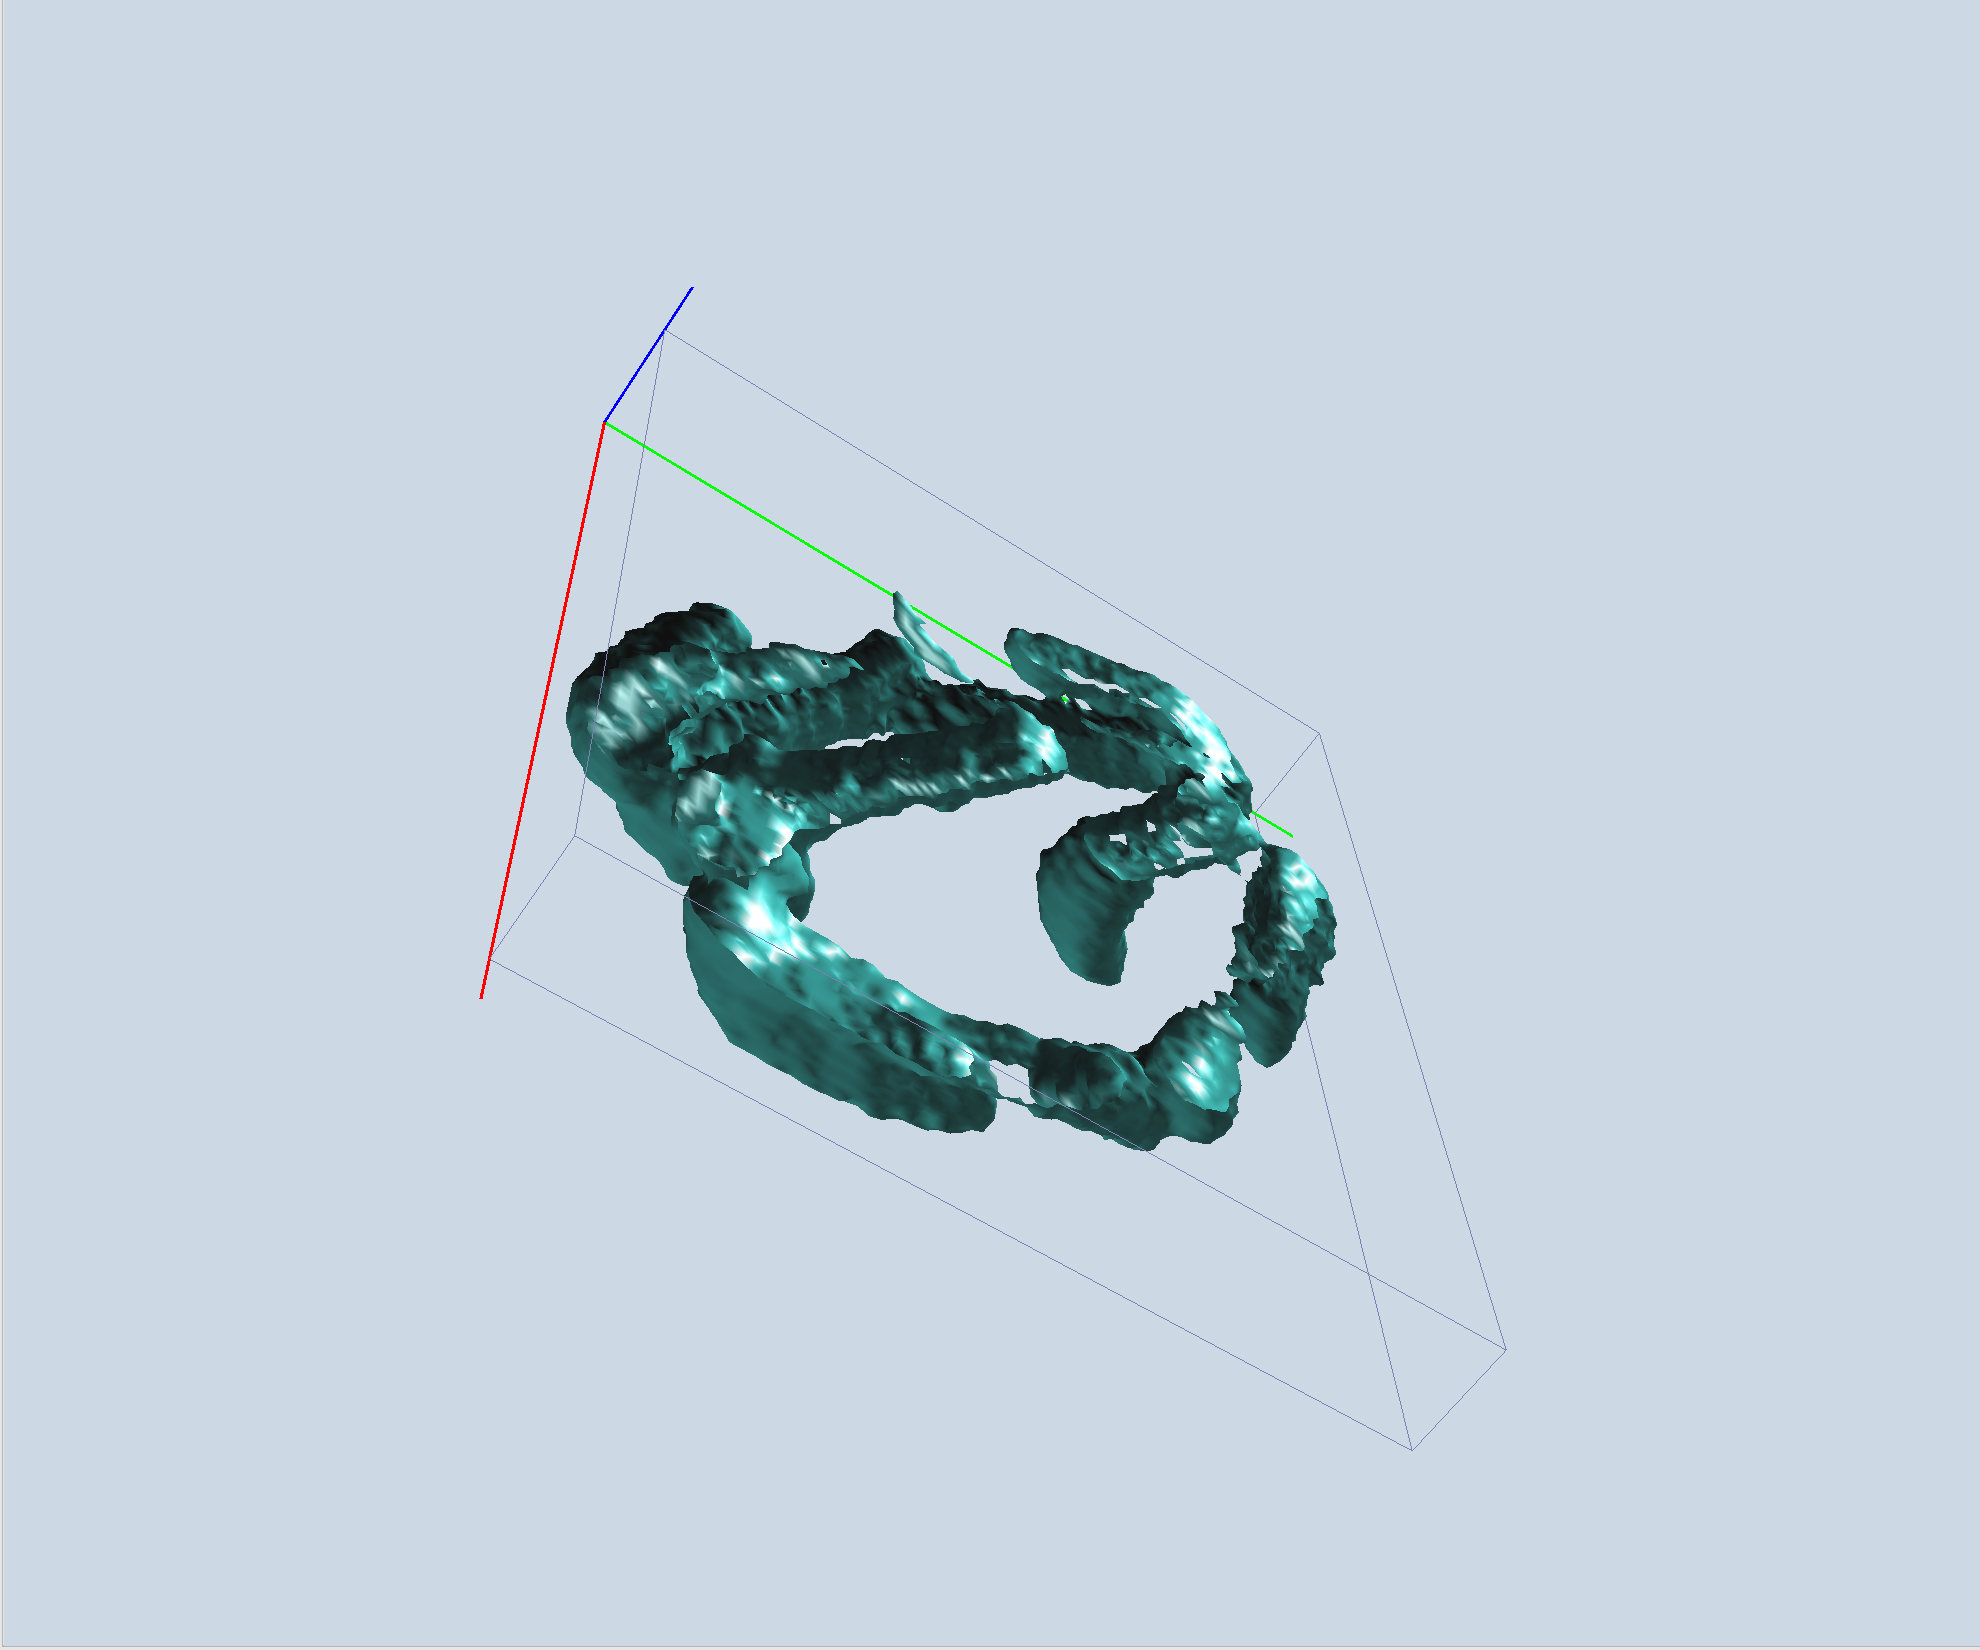
\includegraphics[width=0.3\linewidth]{Report/Images/6.3.2/0-75,100-sliced.png}
    \caption{Threshold: 0-75, mesh density:100, original (left), rotated (middle), cross-section(right)}
    \label{fig:surface_vis_0_75-100}
\end{figure}


\begin{figure}[h!]
    \centering
    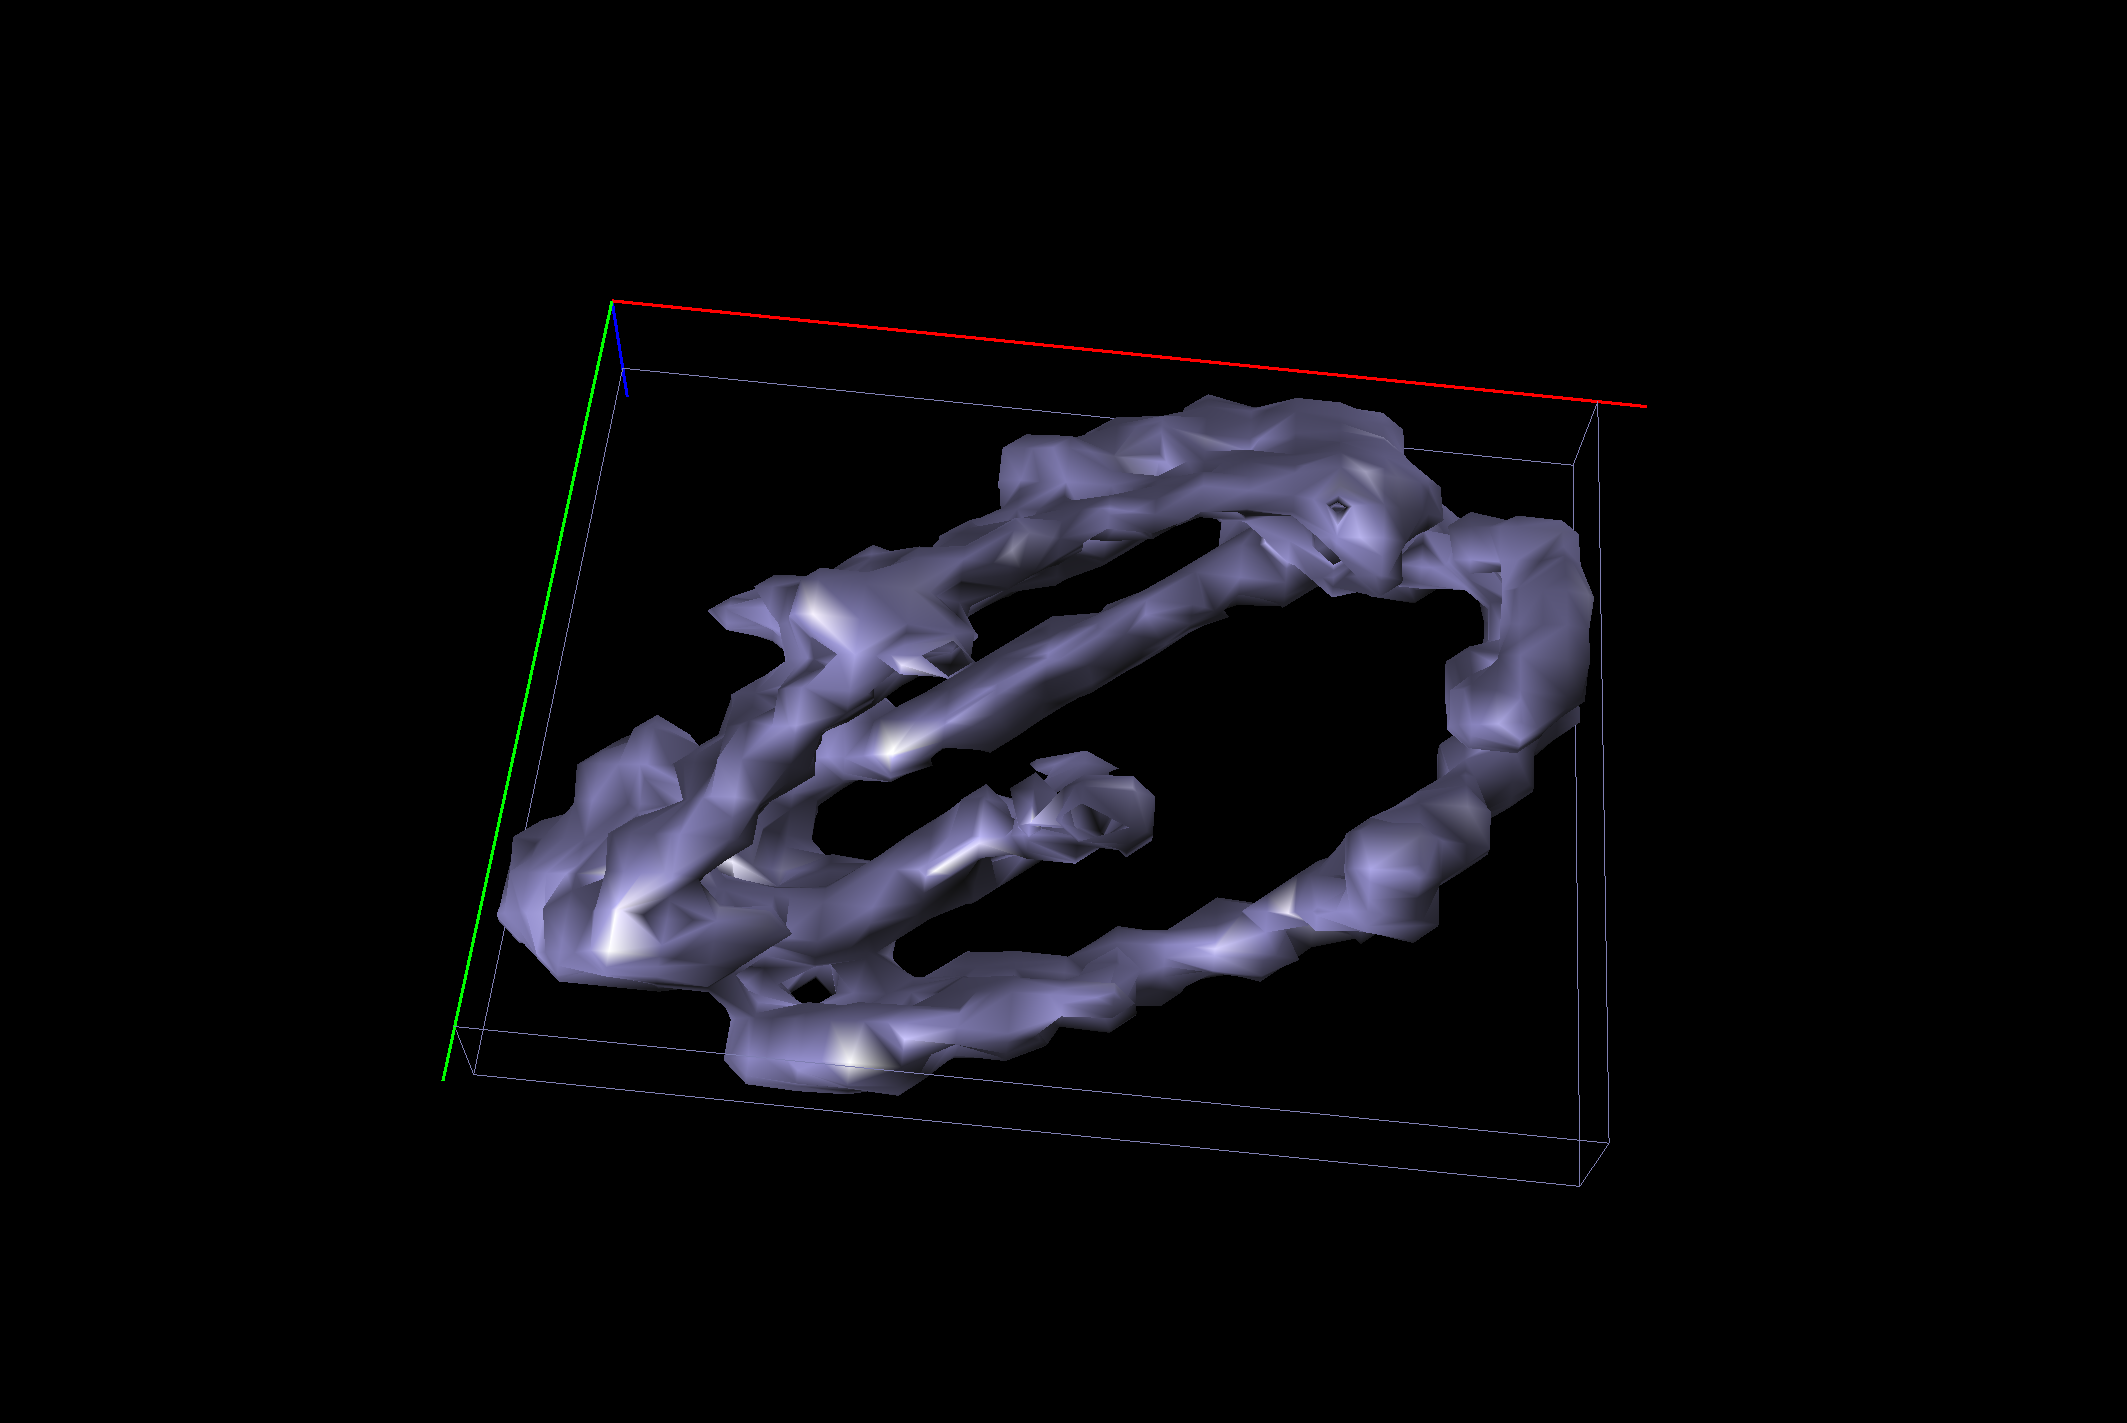
\includegraphics[width=0.3\linewidth]{Report/Images/6.3.2/75-150,25.png}
    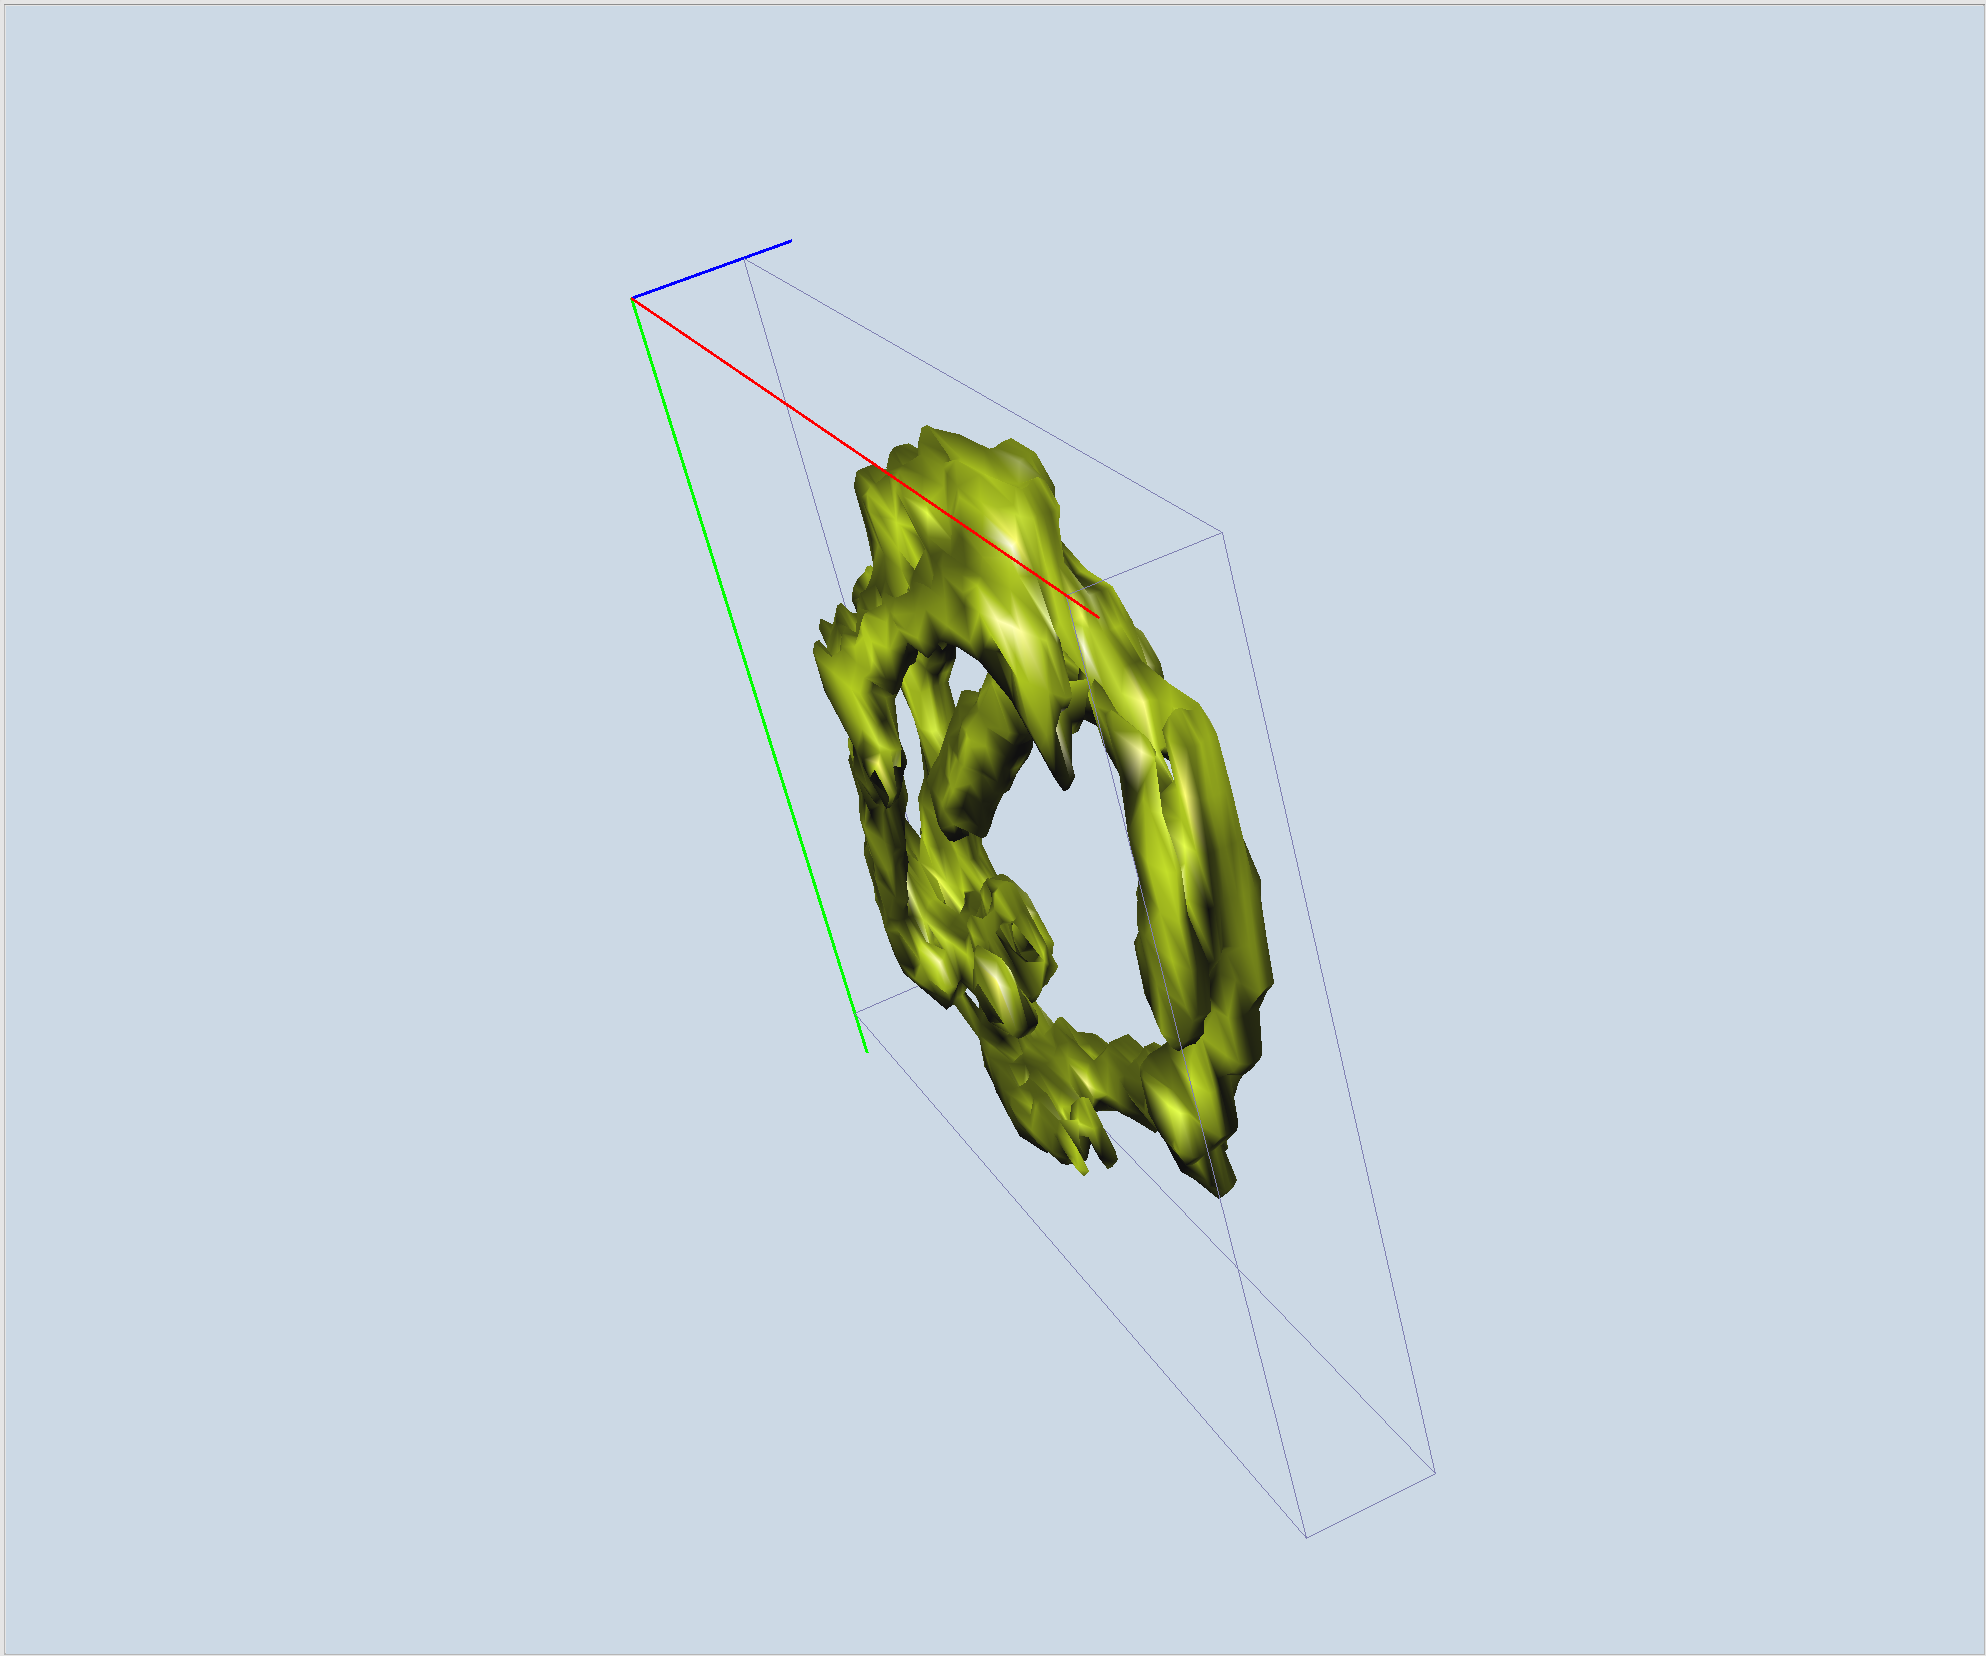
\includegraphics[width=0.3\linewidth]{Report/Images/6.3.2/75-150,25-rotated.png}
    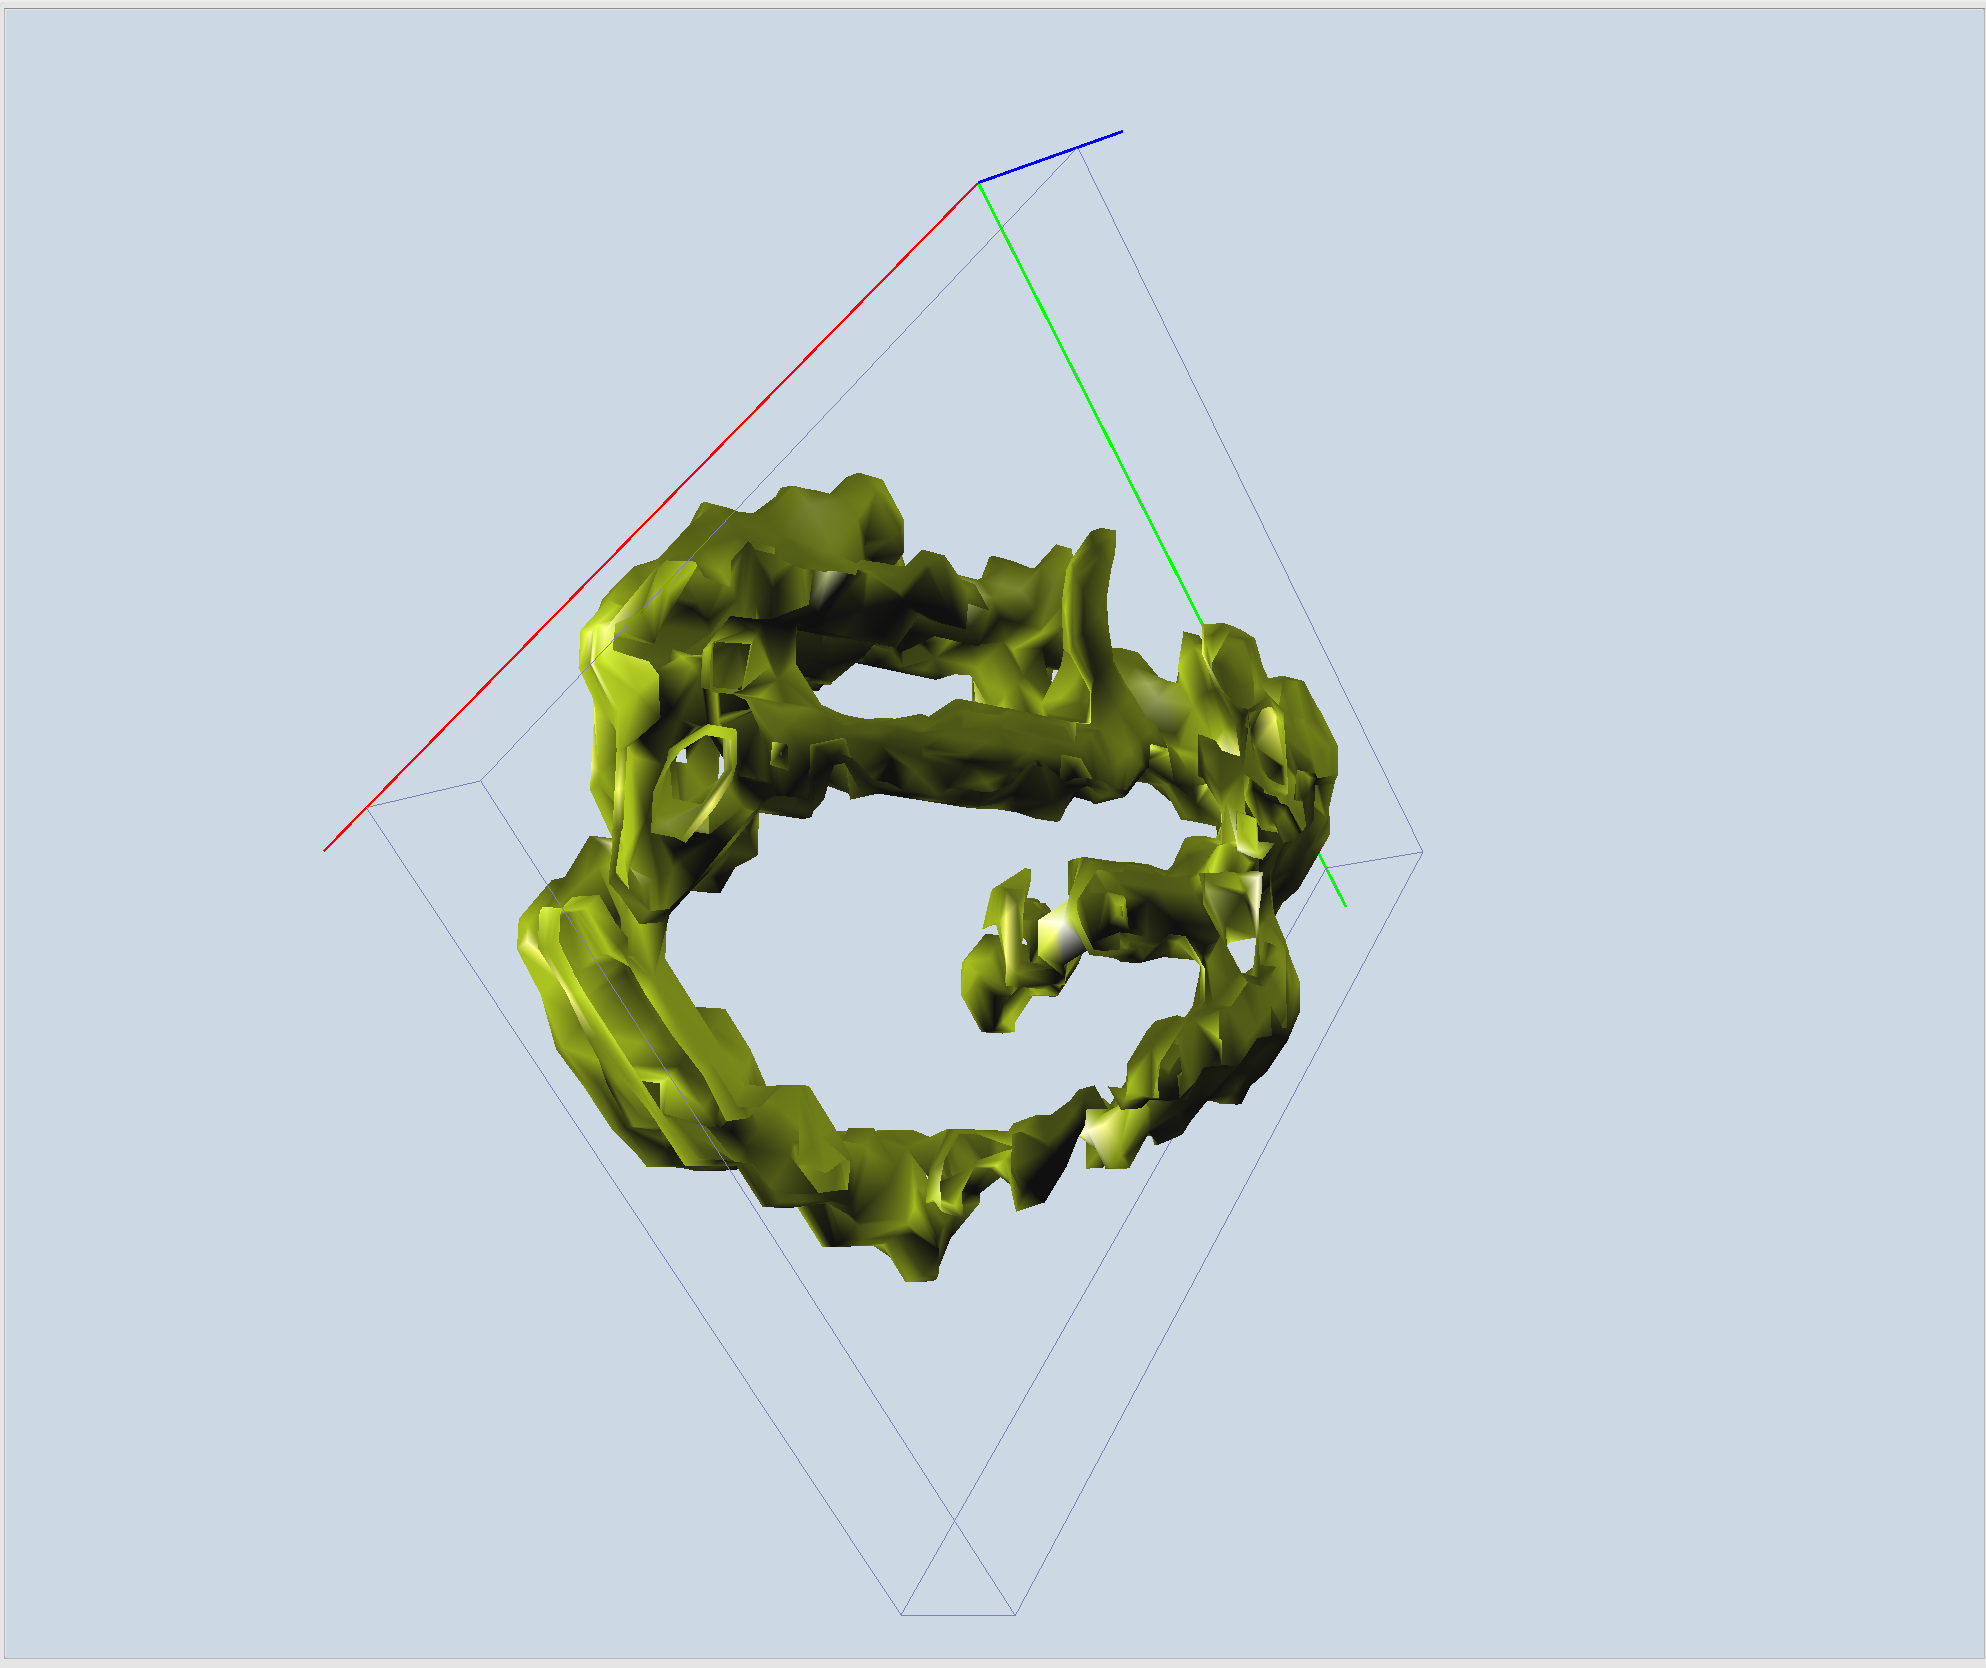
\includegraphics[width=0.3\linewidth]{Report/Images/6.3.2/75-150,25-sliced.png}
    \caption{Threshold: 75-150, mesh density:25, original (left), rotated (middle), cross-section(right)}
    \label{fig:surface_vis_75_150-25}
\end{figure}


\begin{figure}[h!]
    \centering
    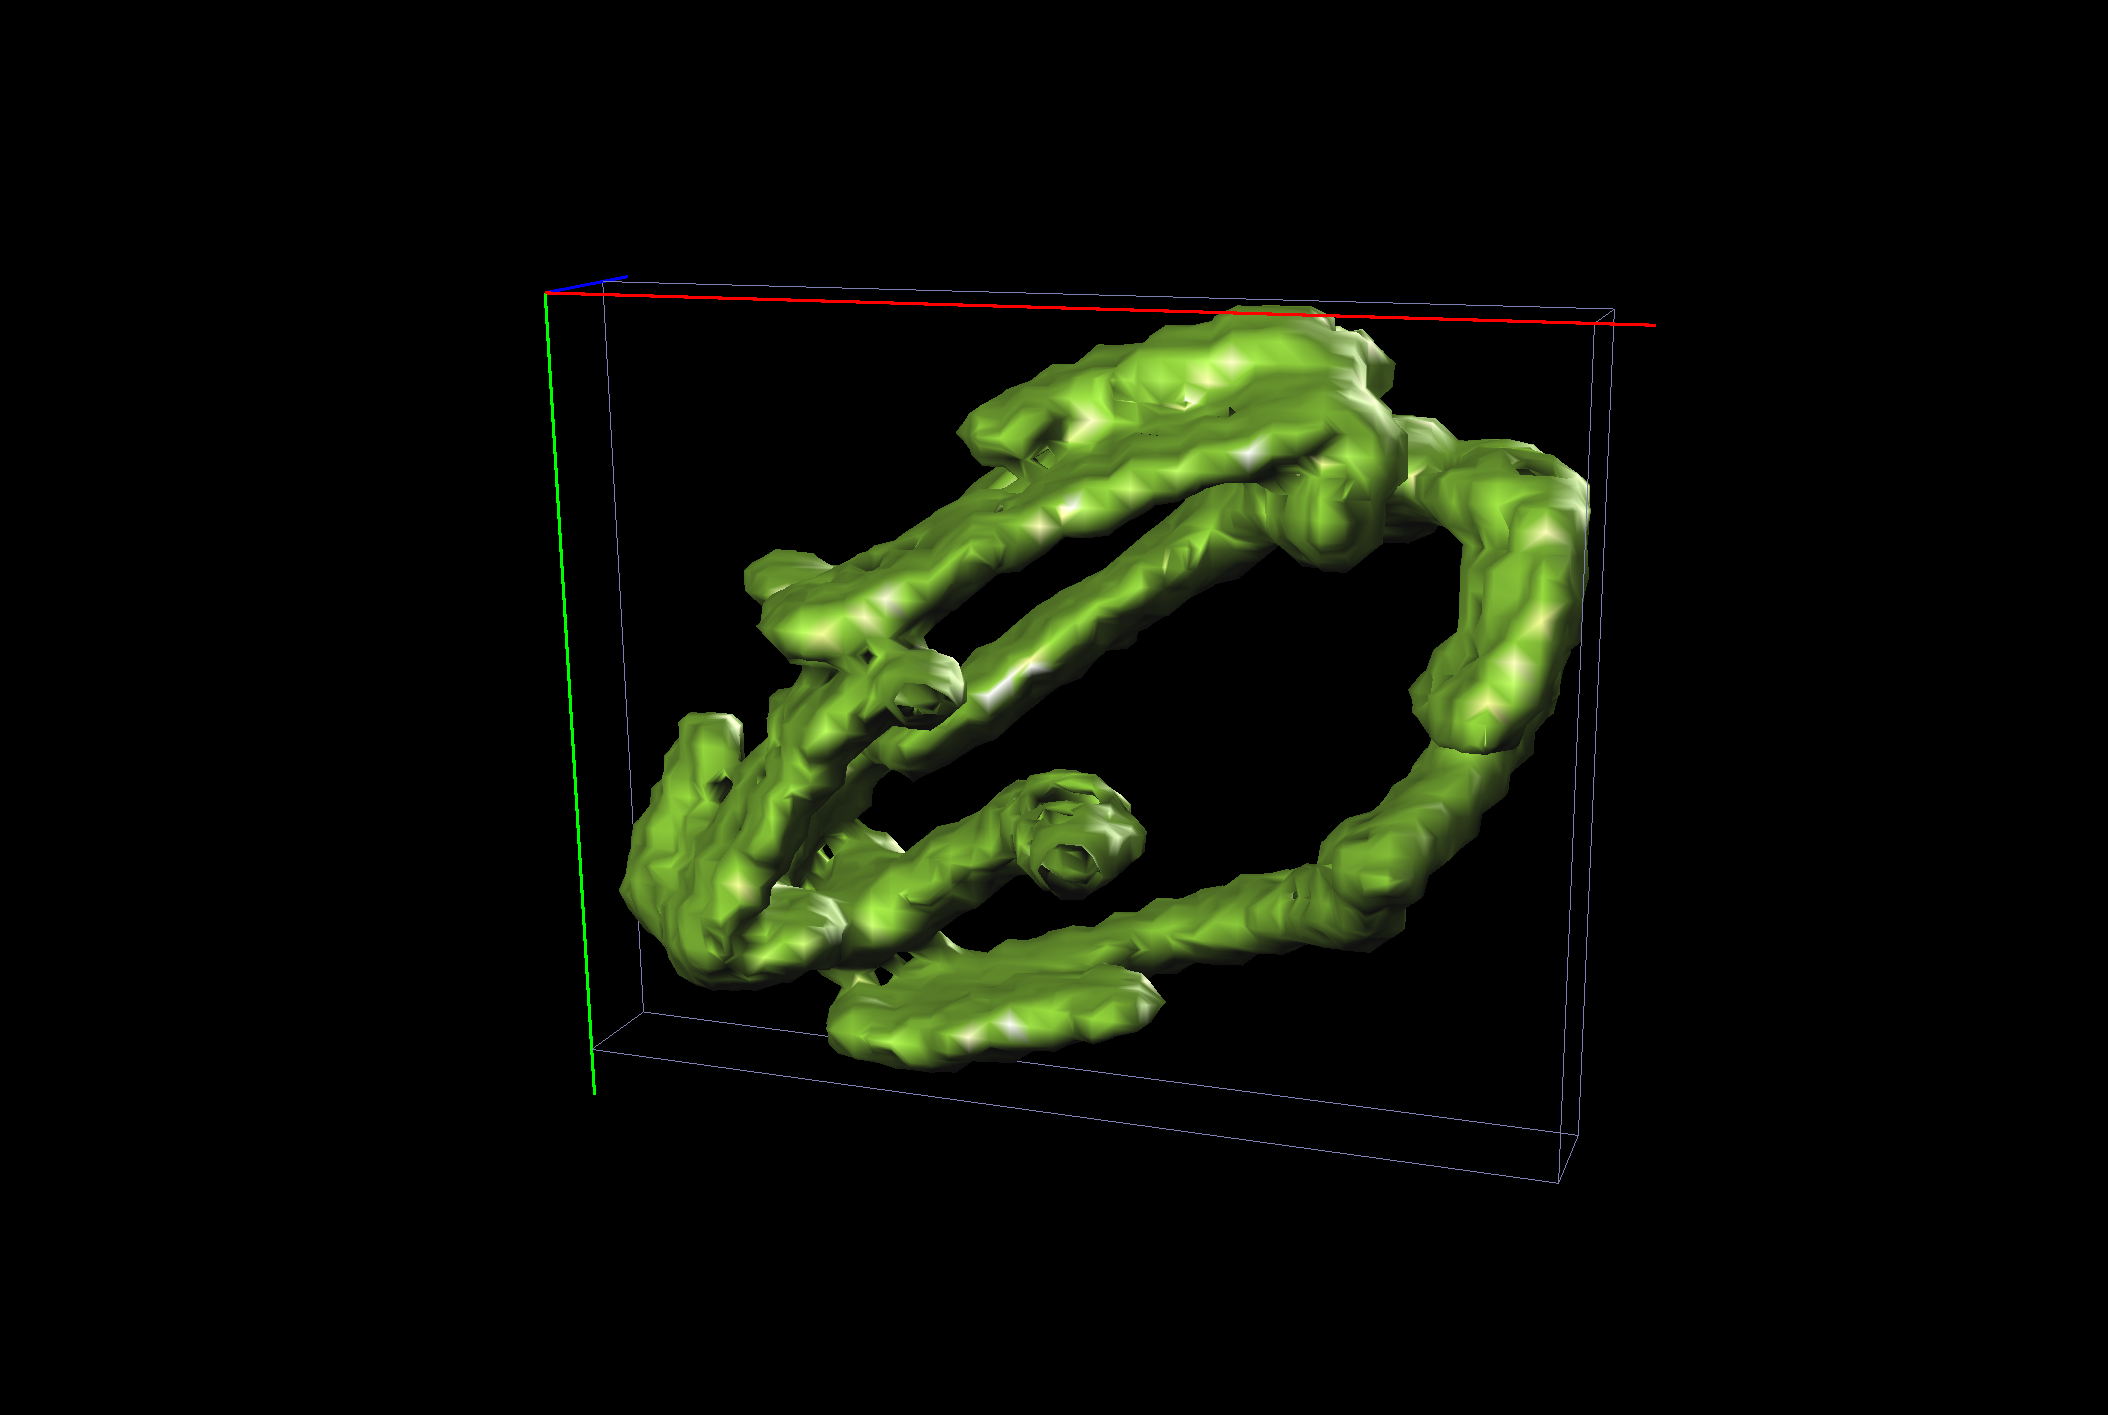
\includegraphics[width=0.3\linewidth]{Report/Images/6.3.2/75-150,50.png}
    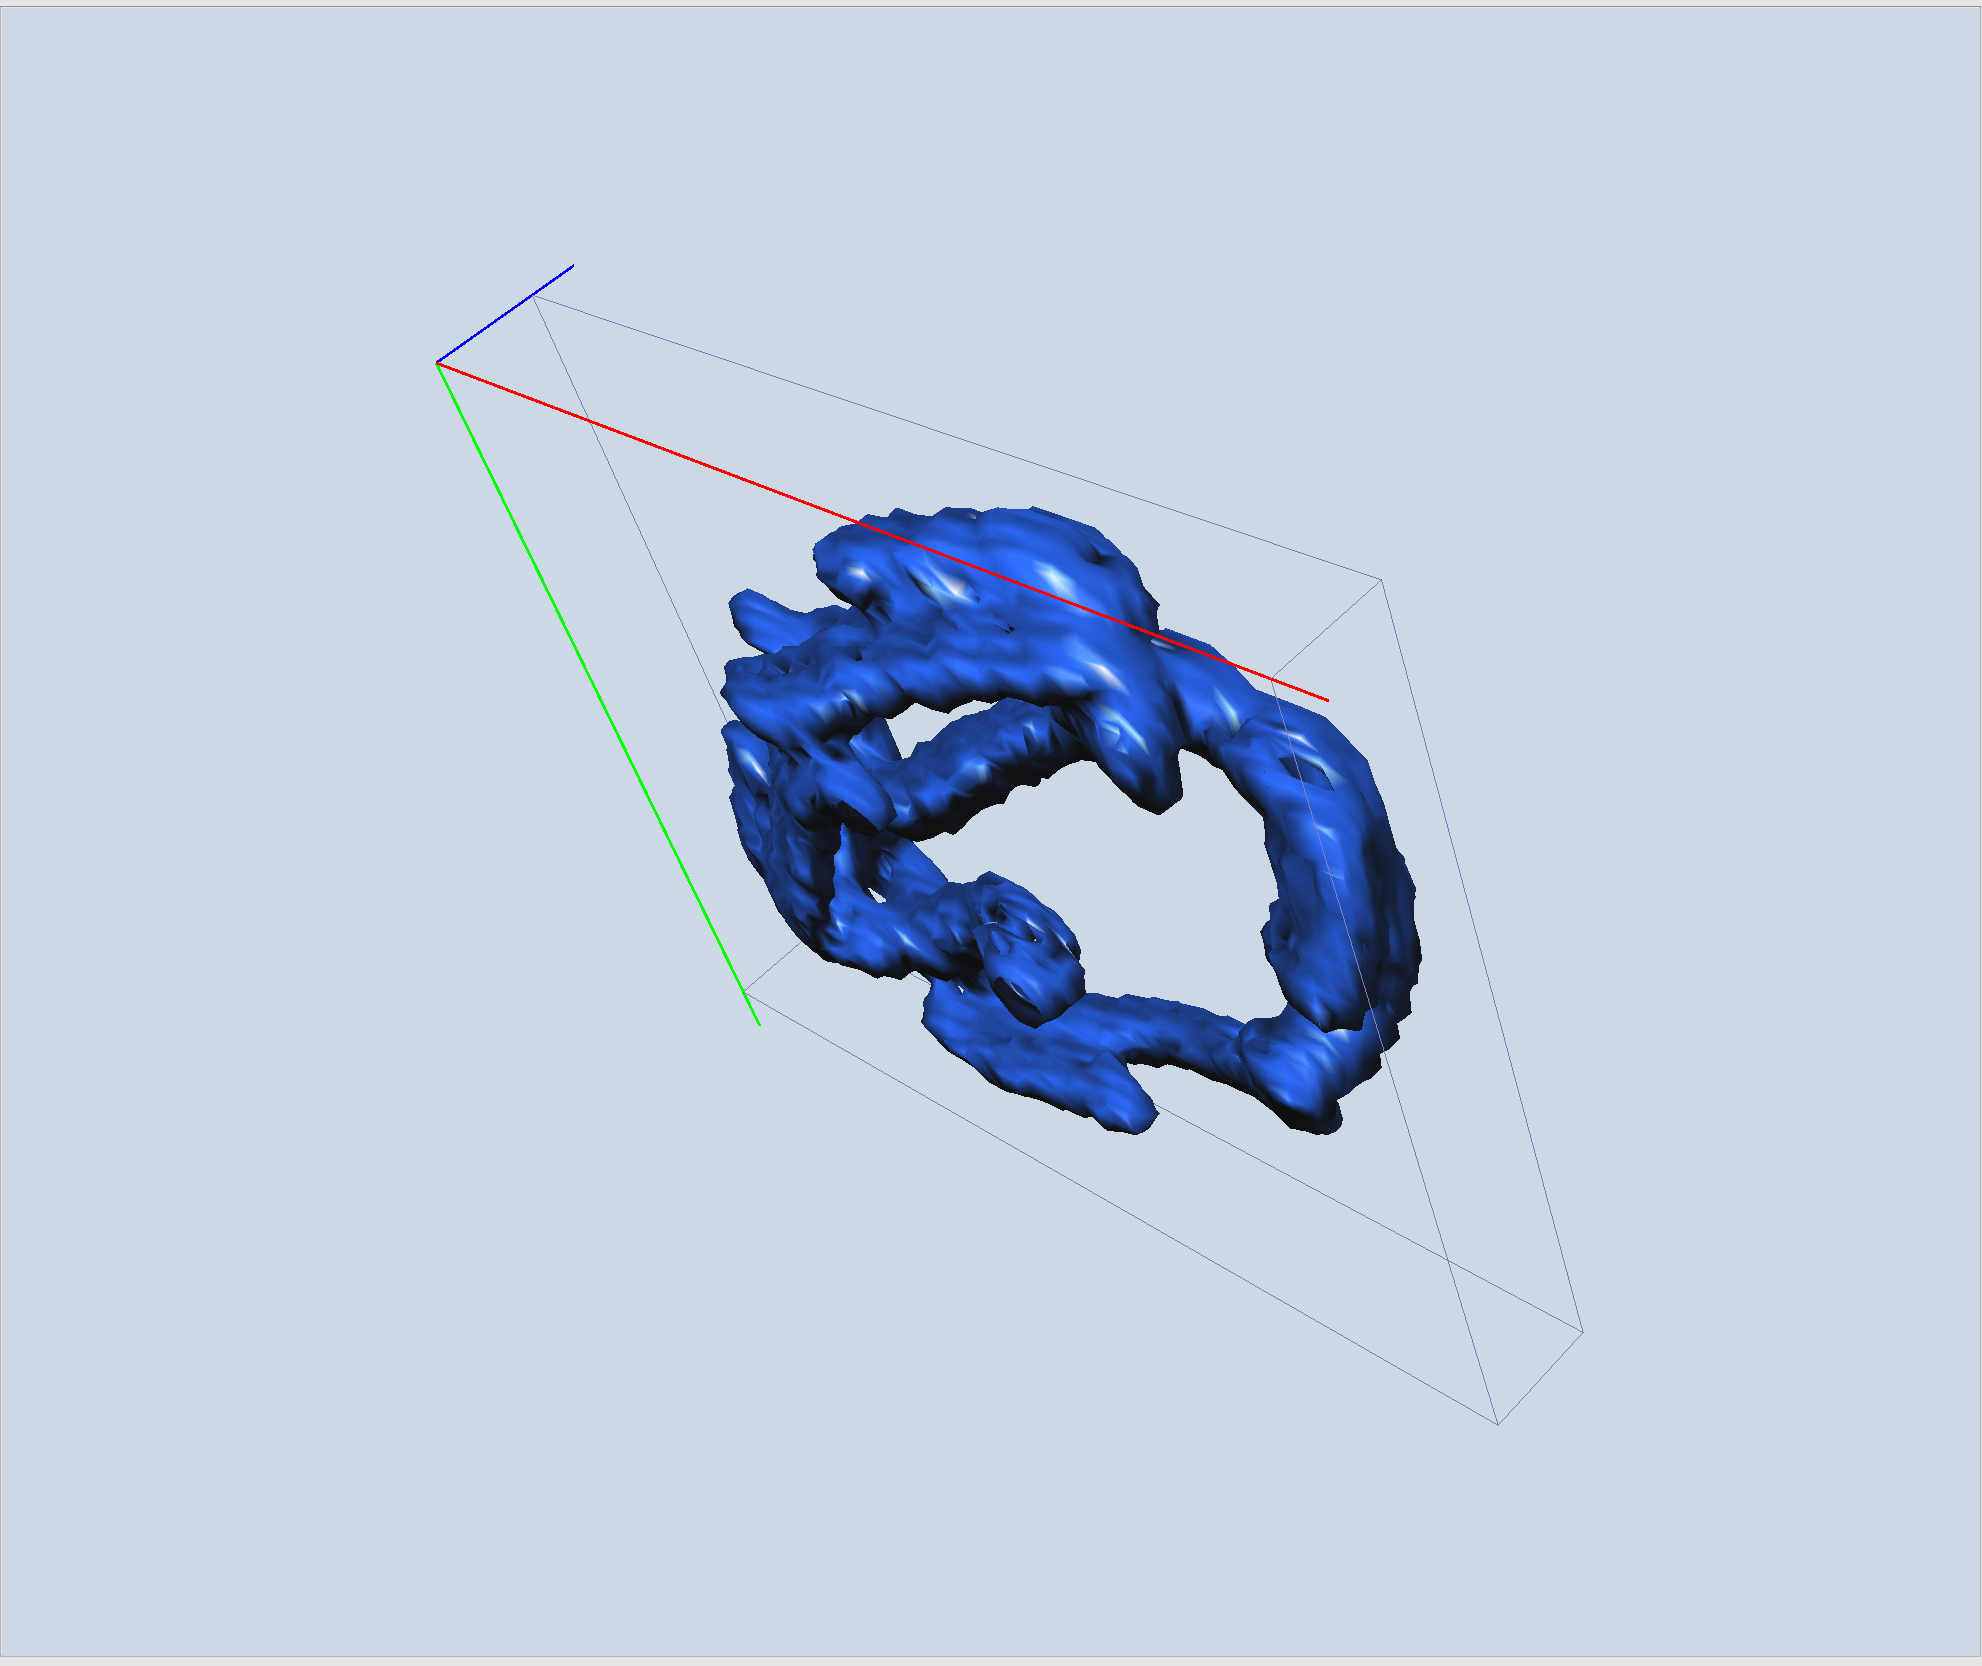
\includegraphics[width=0.3\linewidth]{Report/Images/6.3.2/75-150,50-rotated.png}
    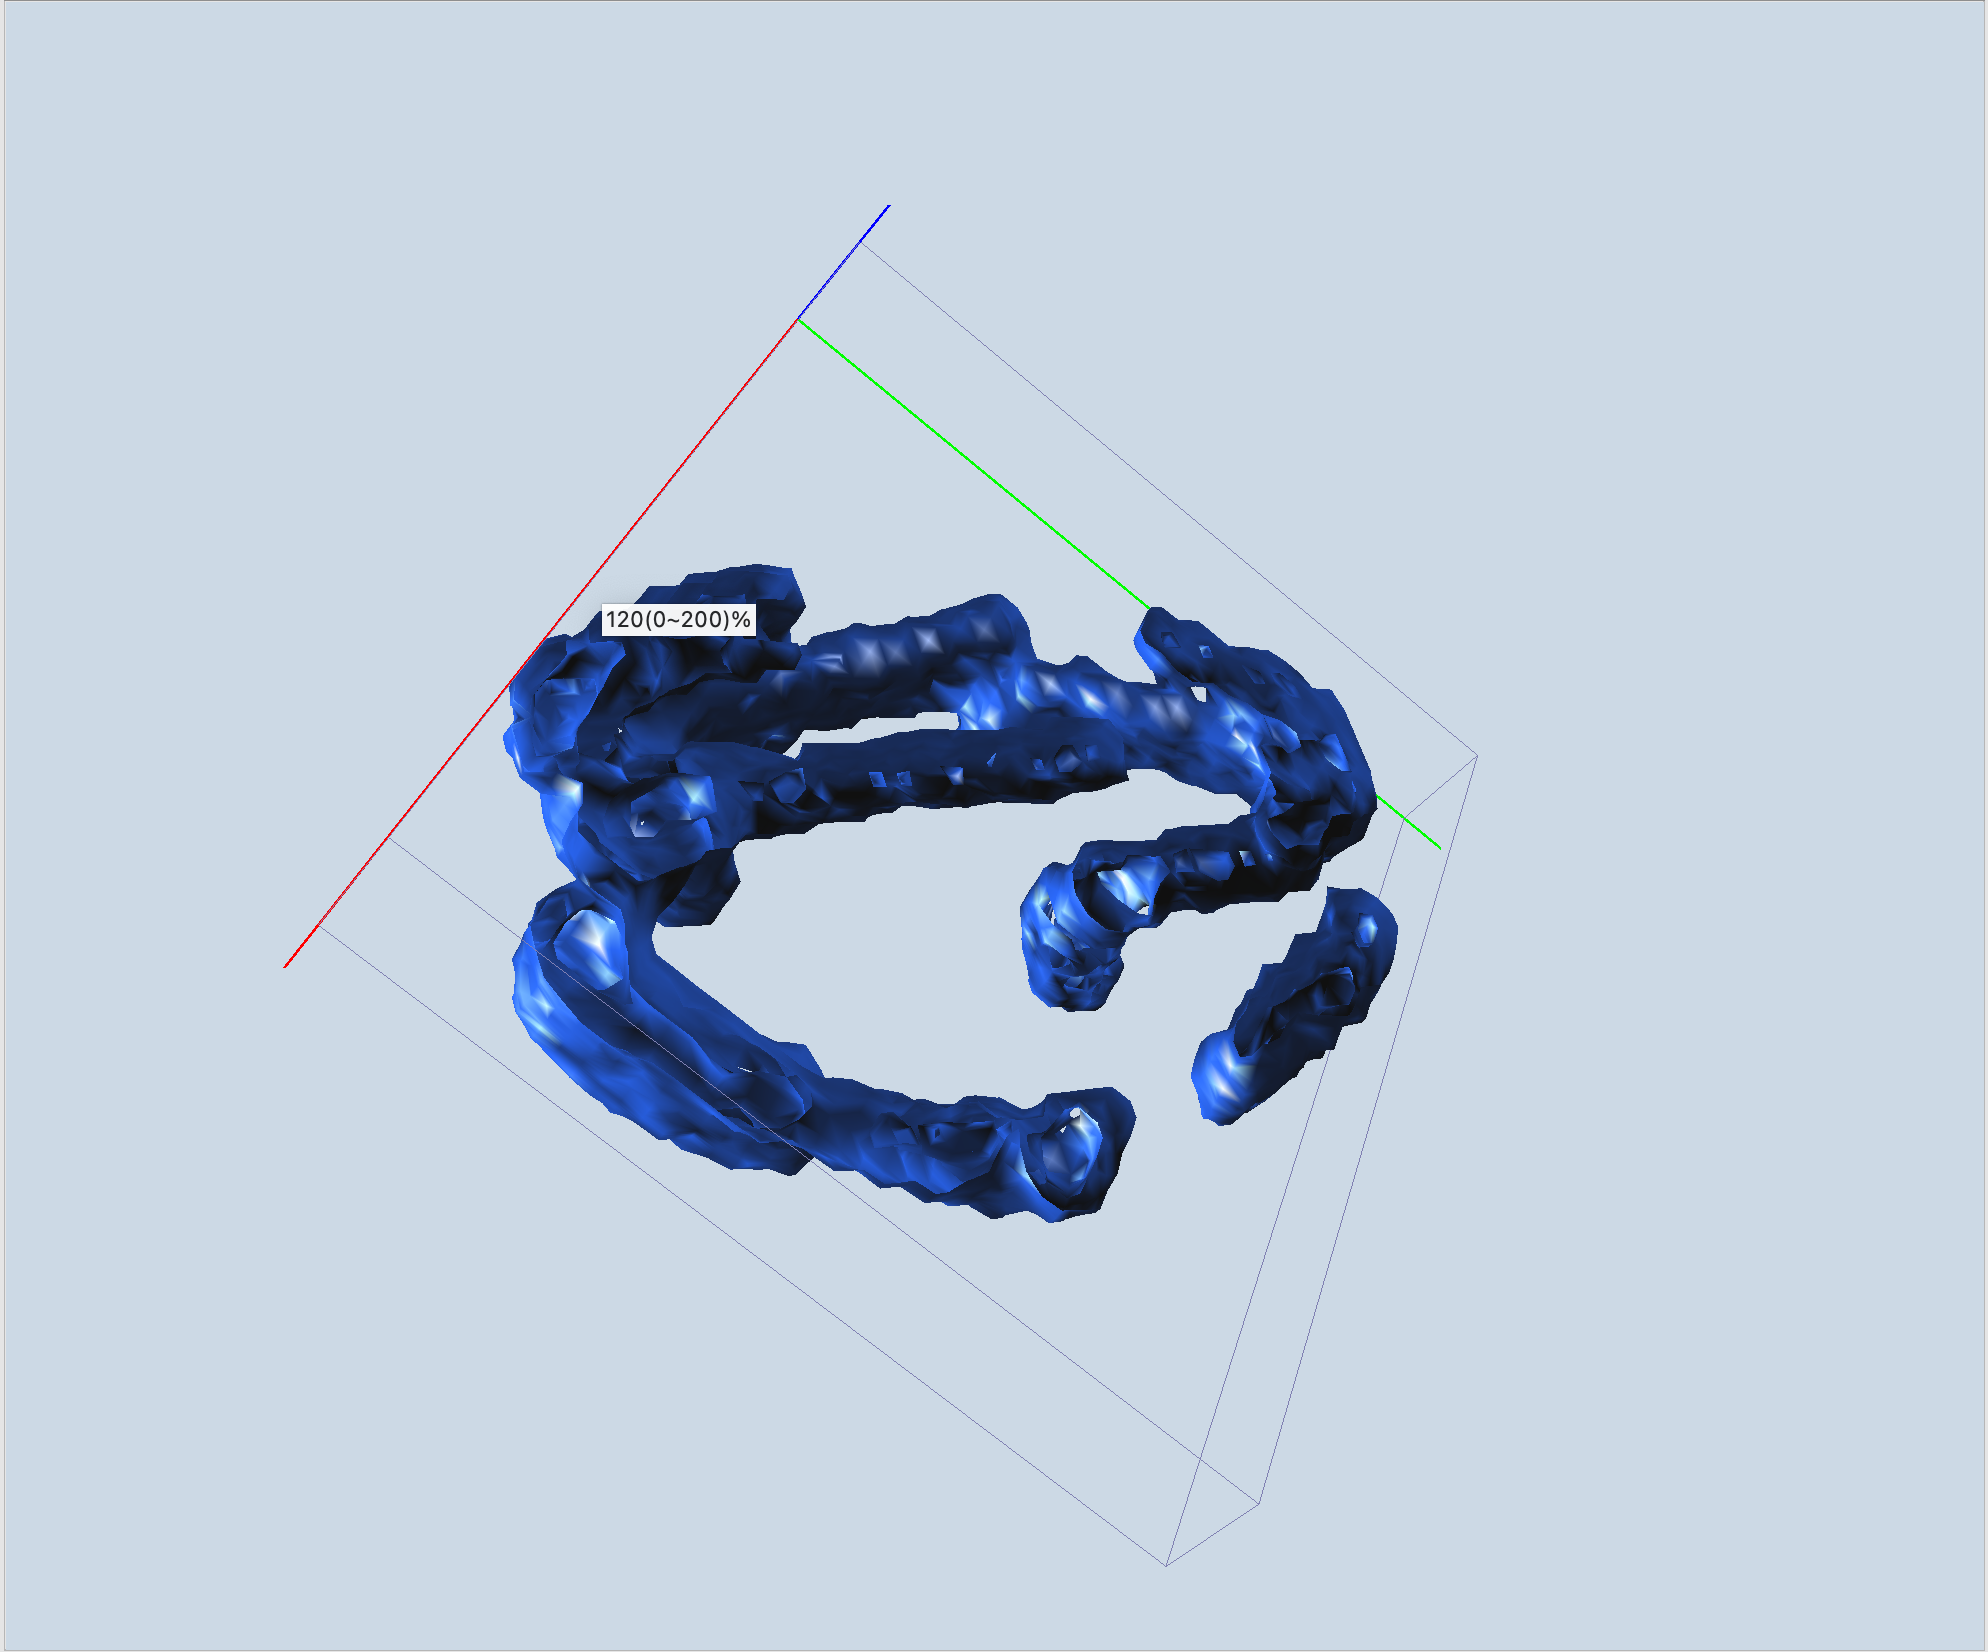
\includegraphics[width=0.3\linewidth]{Report/Images/6.3.2/75-150,50-sliced.png}
    \caption{Threshold: 75-150, mesh density:50, original (left), rotated (middle), cross-section(right)}
    \label{fig:surface_vis_75_150-50}
\end{figure}


\begin{figure}[h!]
    \centering
    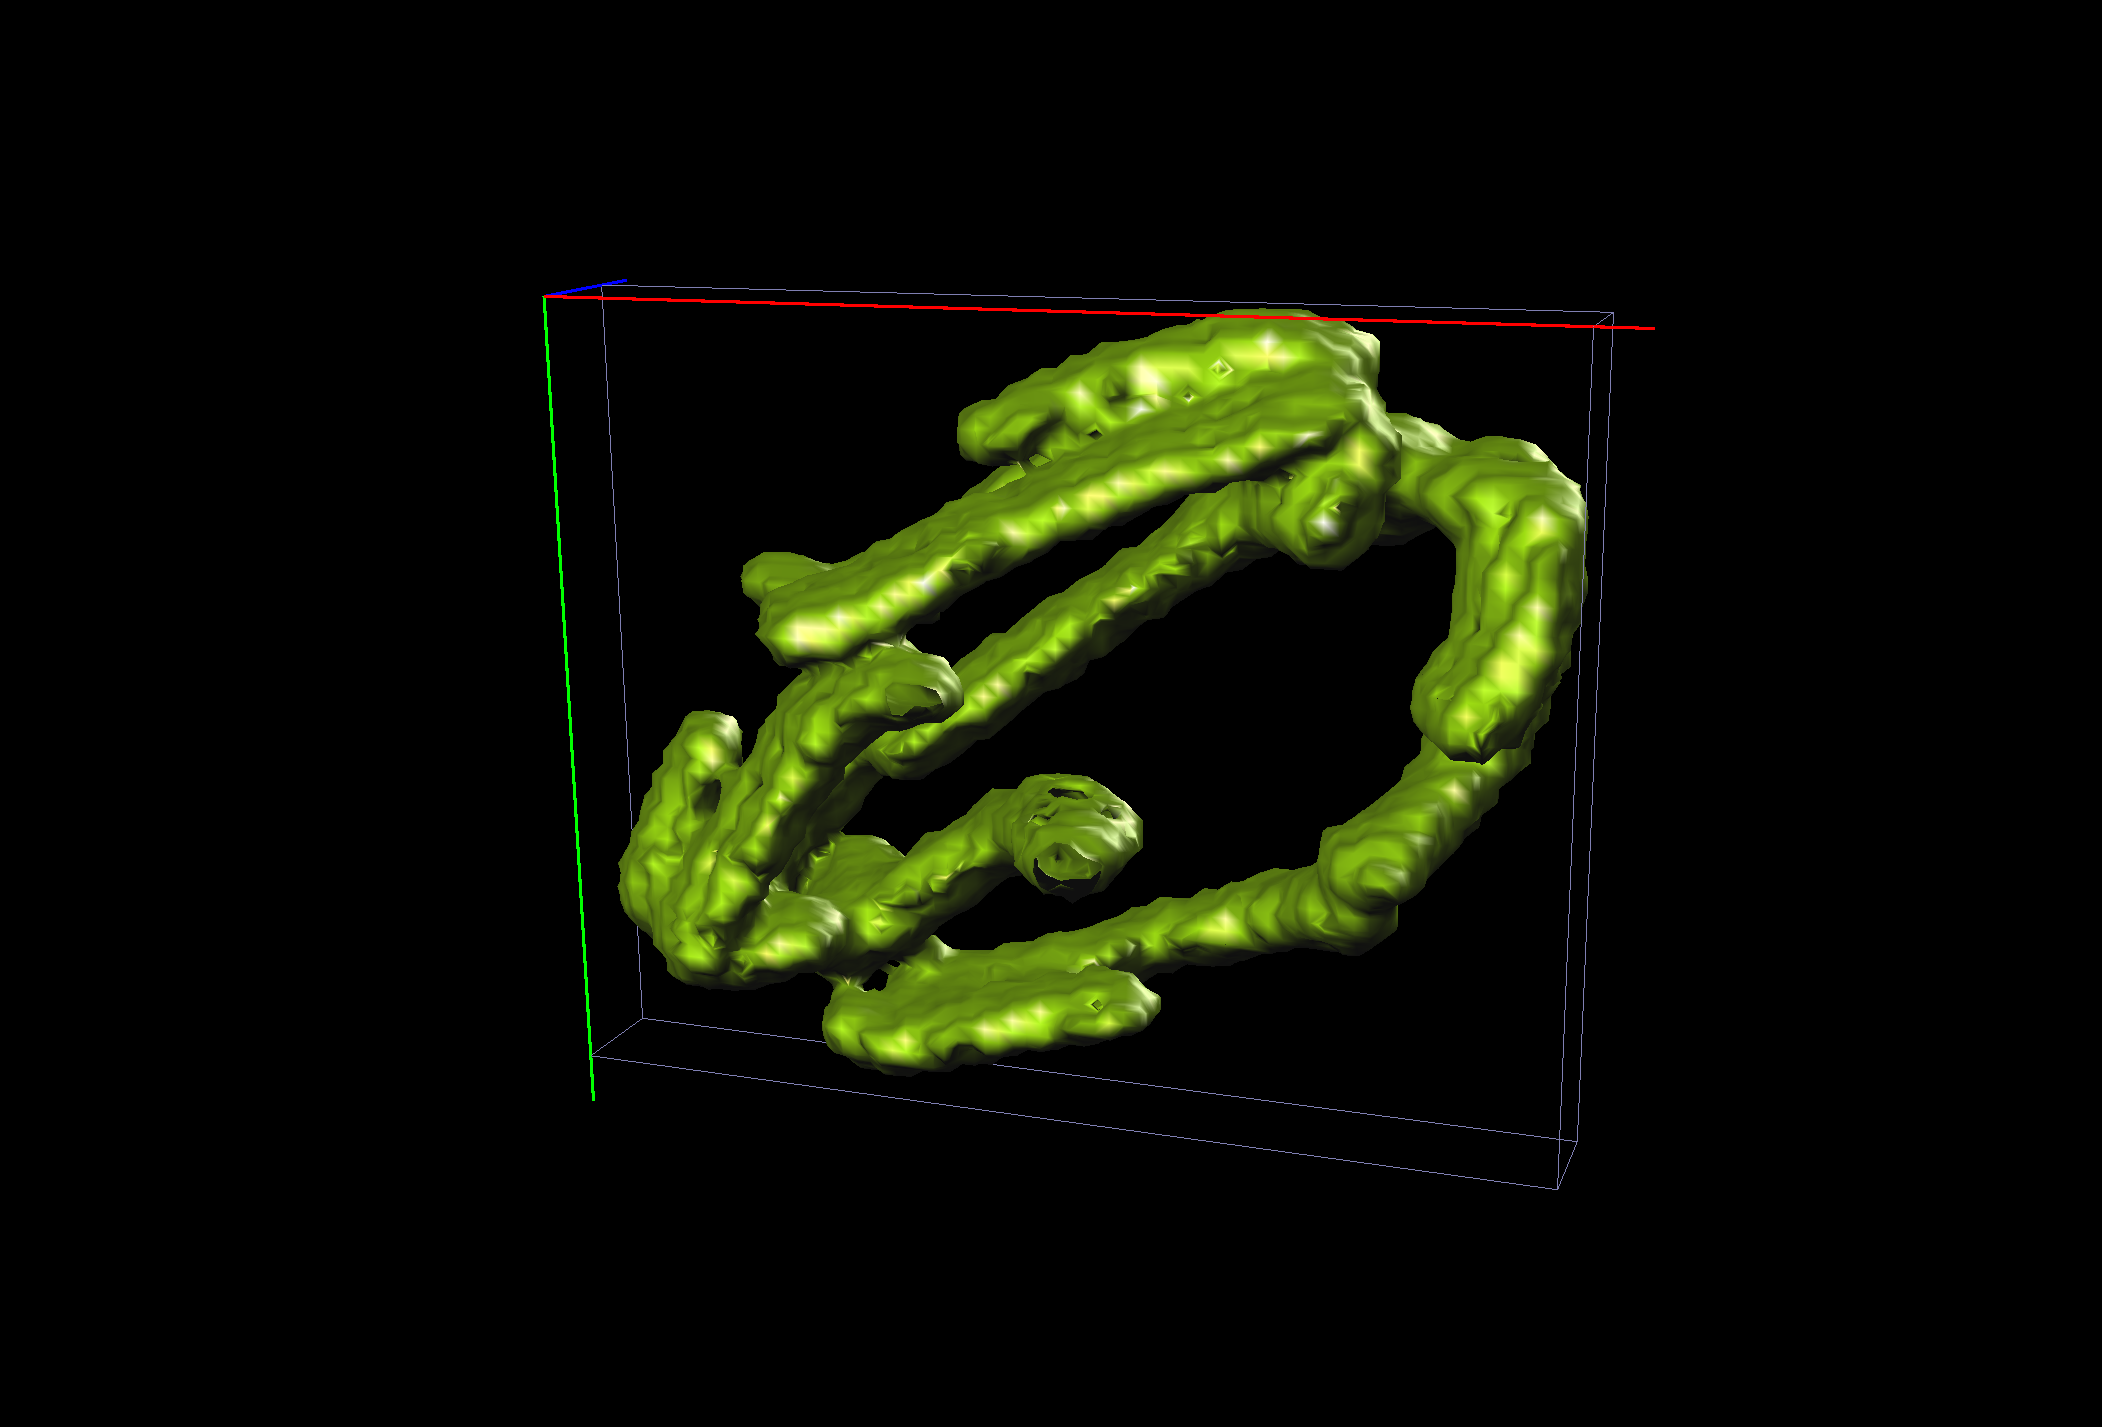
\includegraphics[width=0.3\linewidth]{Report/Images/6.3.2/75-150,75.png}
    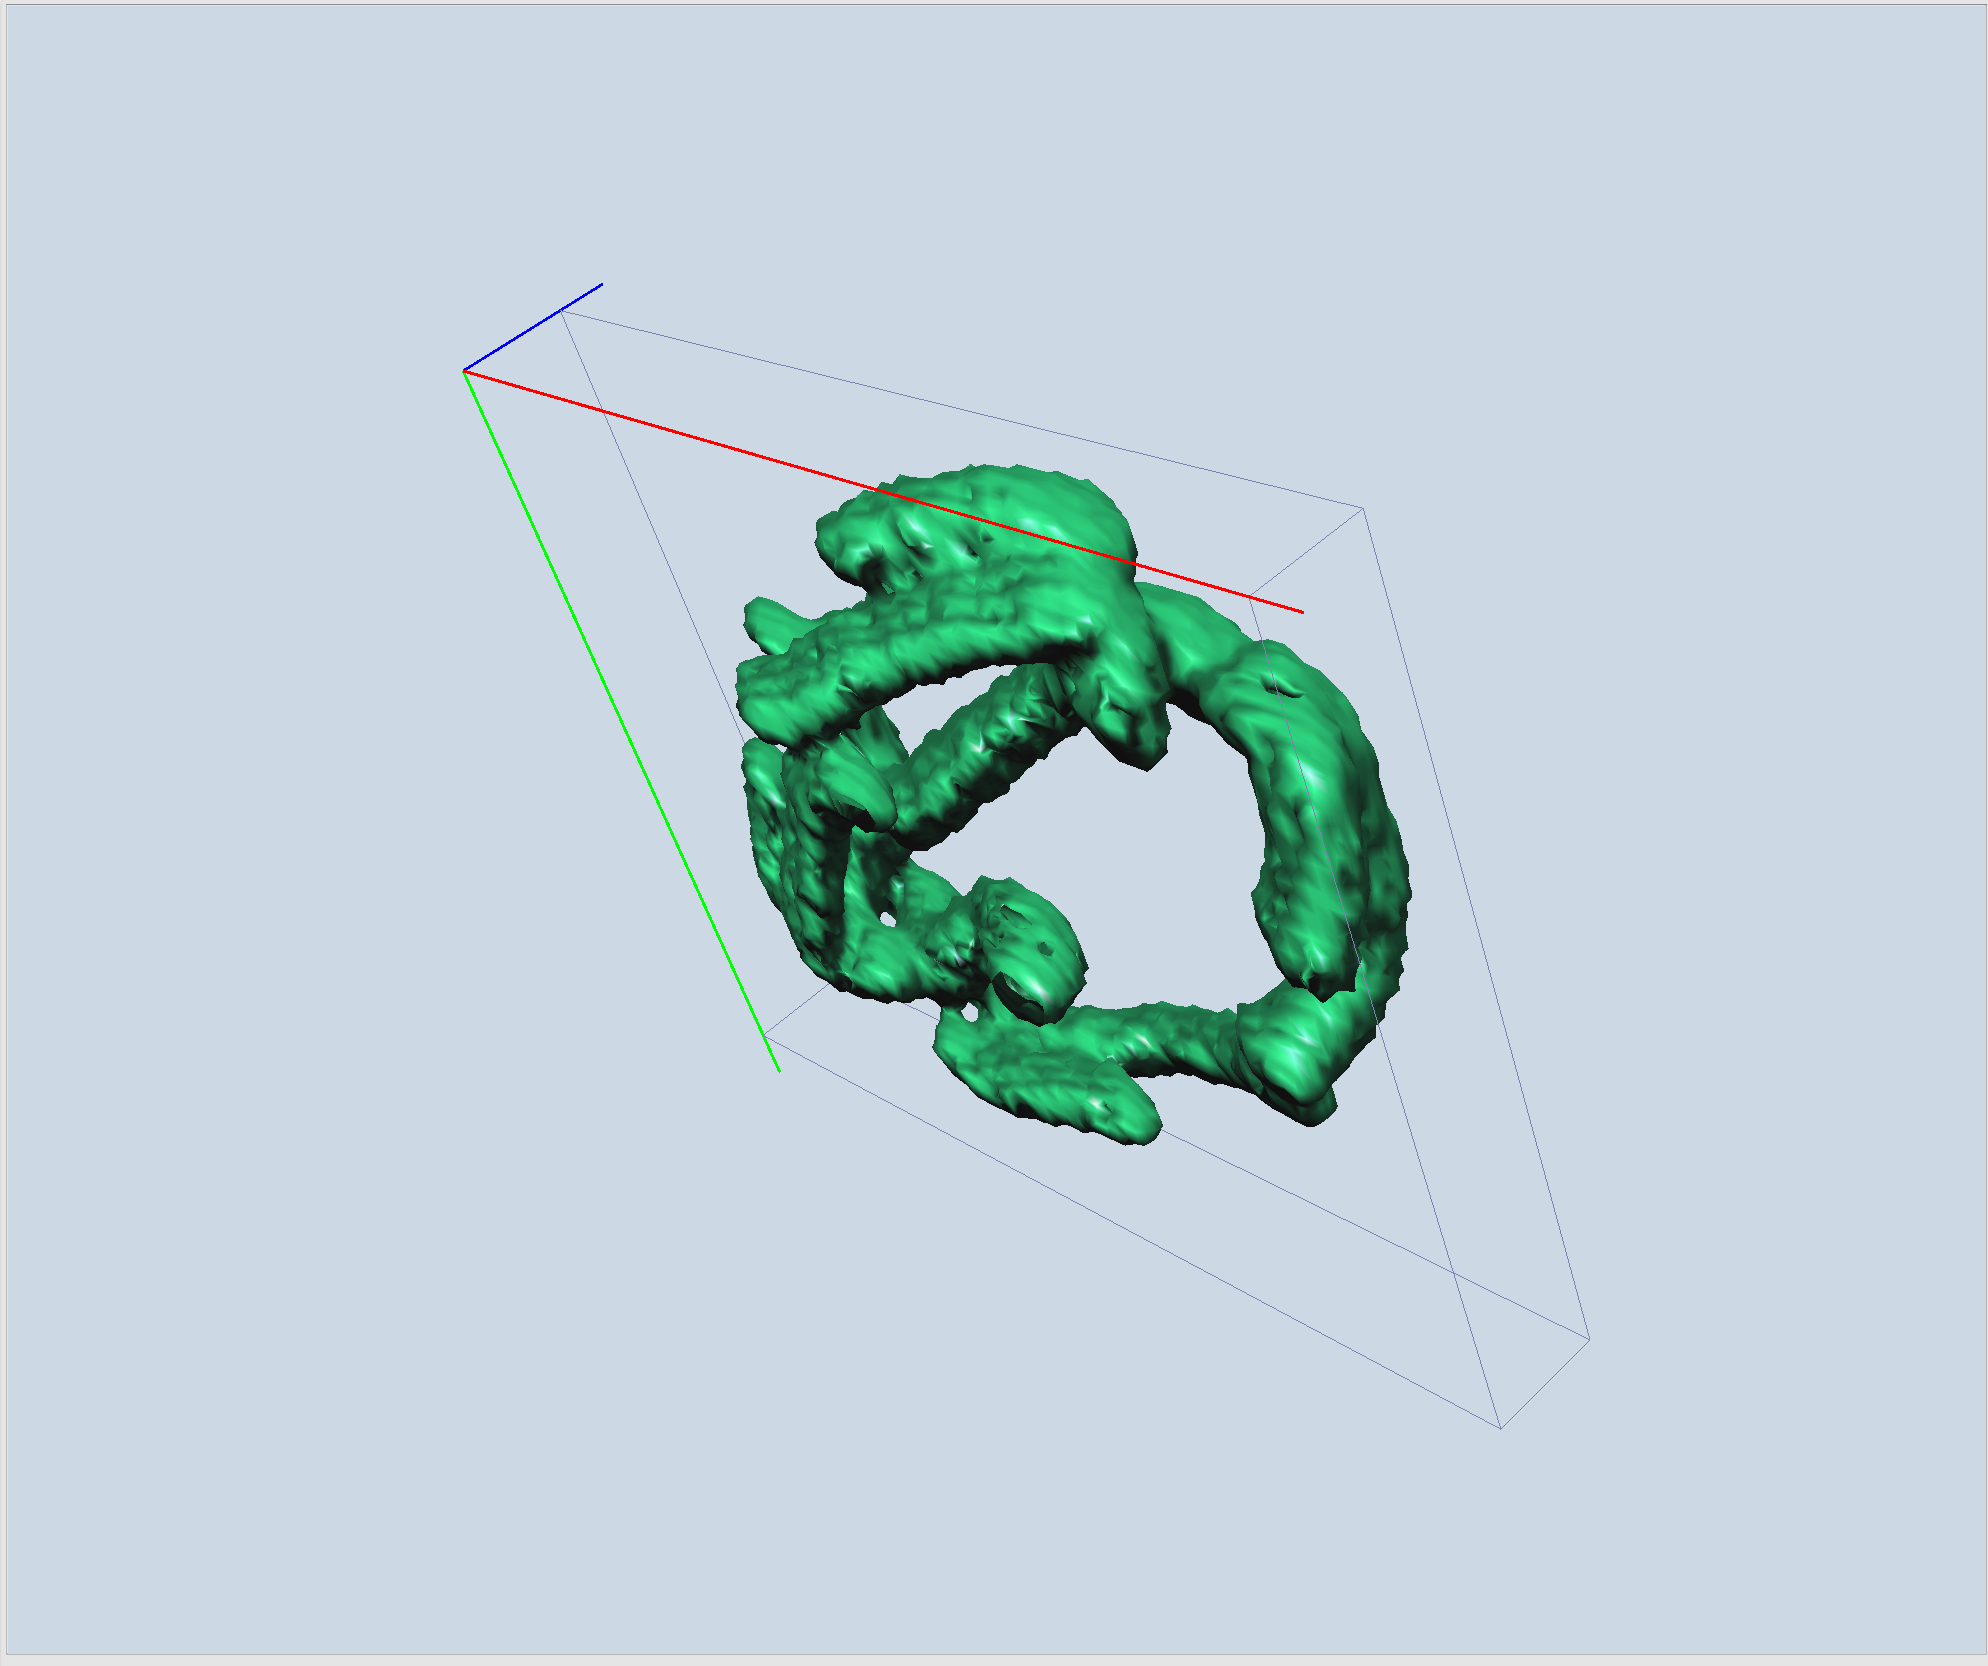
\includegraphics[width=0.3\linewidth]{Report/Images/6.3.2/75-150,75-rotated.png}
    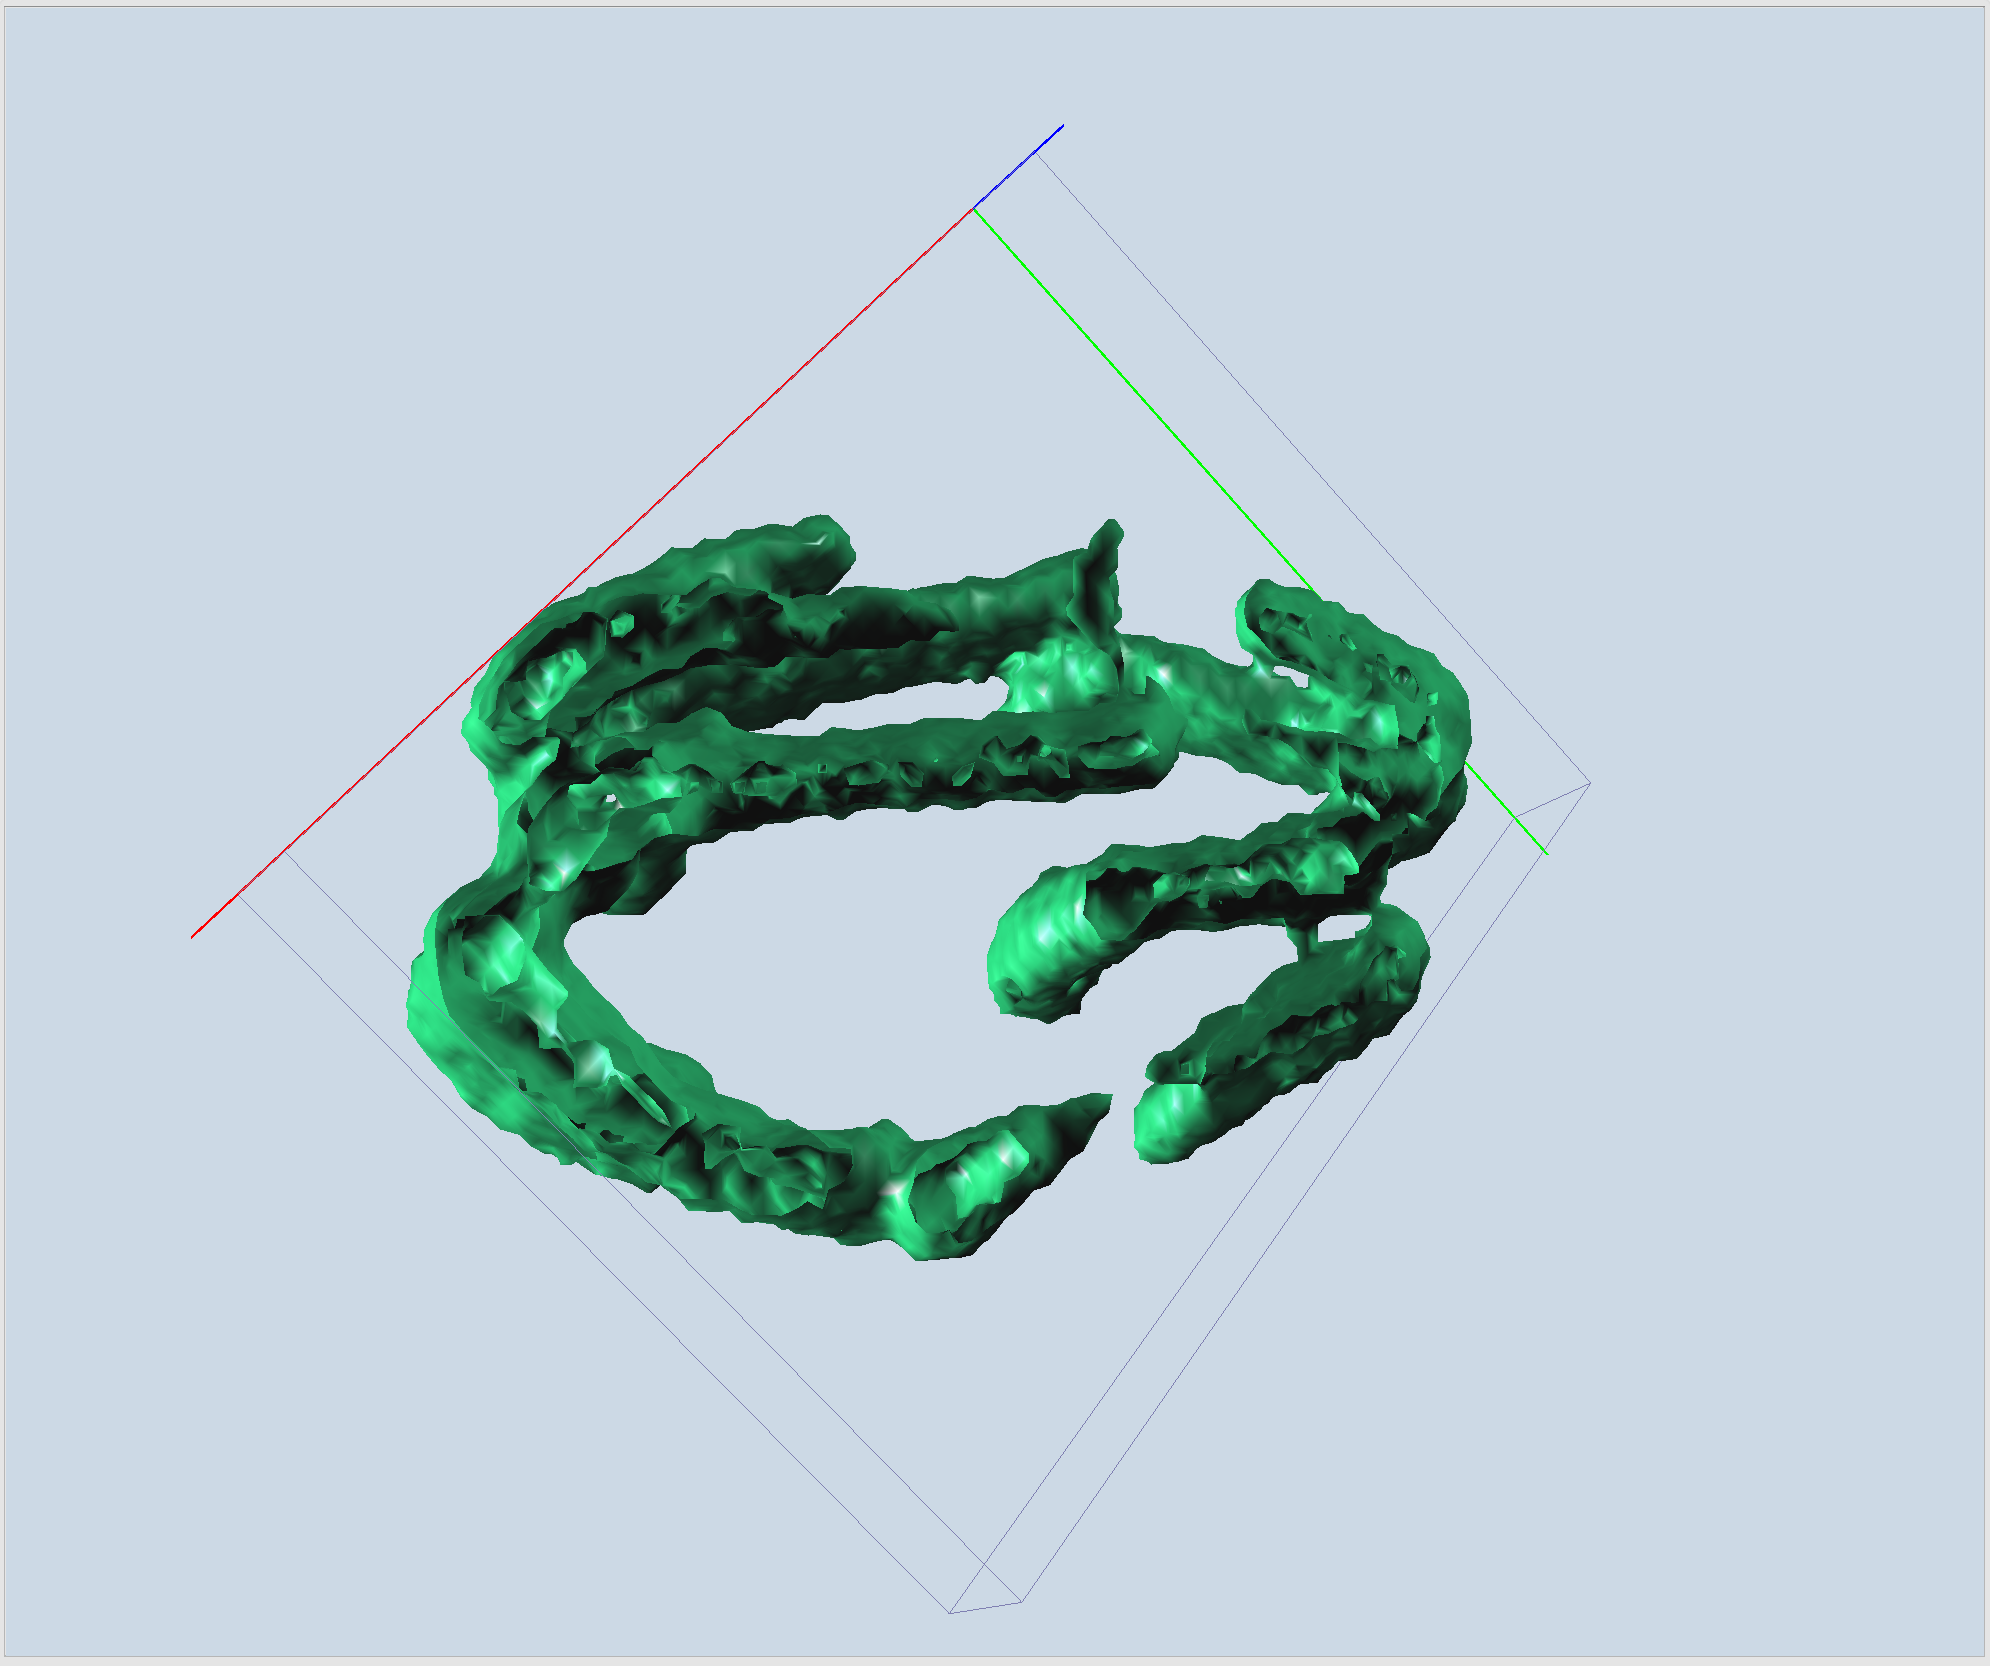
\includegraphics[width=0.3\linewidth]{Report/Images/6.3.2/75-150,75-sliced.png}
    \caption{Threshold: 75-150, mesh density:75, original (left), rotated (middle), cross-section(right)}
    \label{fig:surface_vis_75_150-75}
\end{figure}


\begin{figure}[h!]
    \centering
    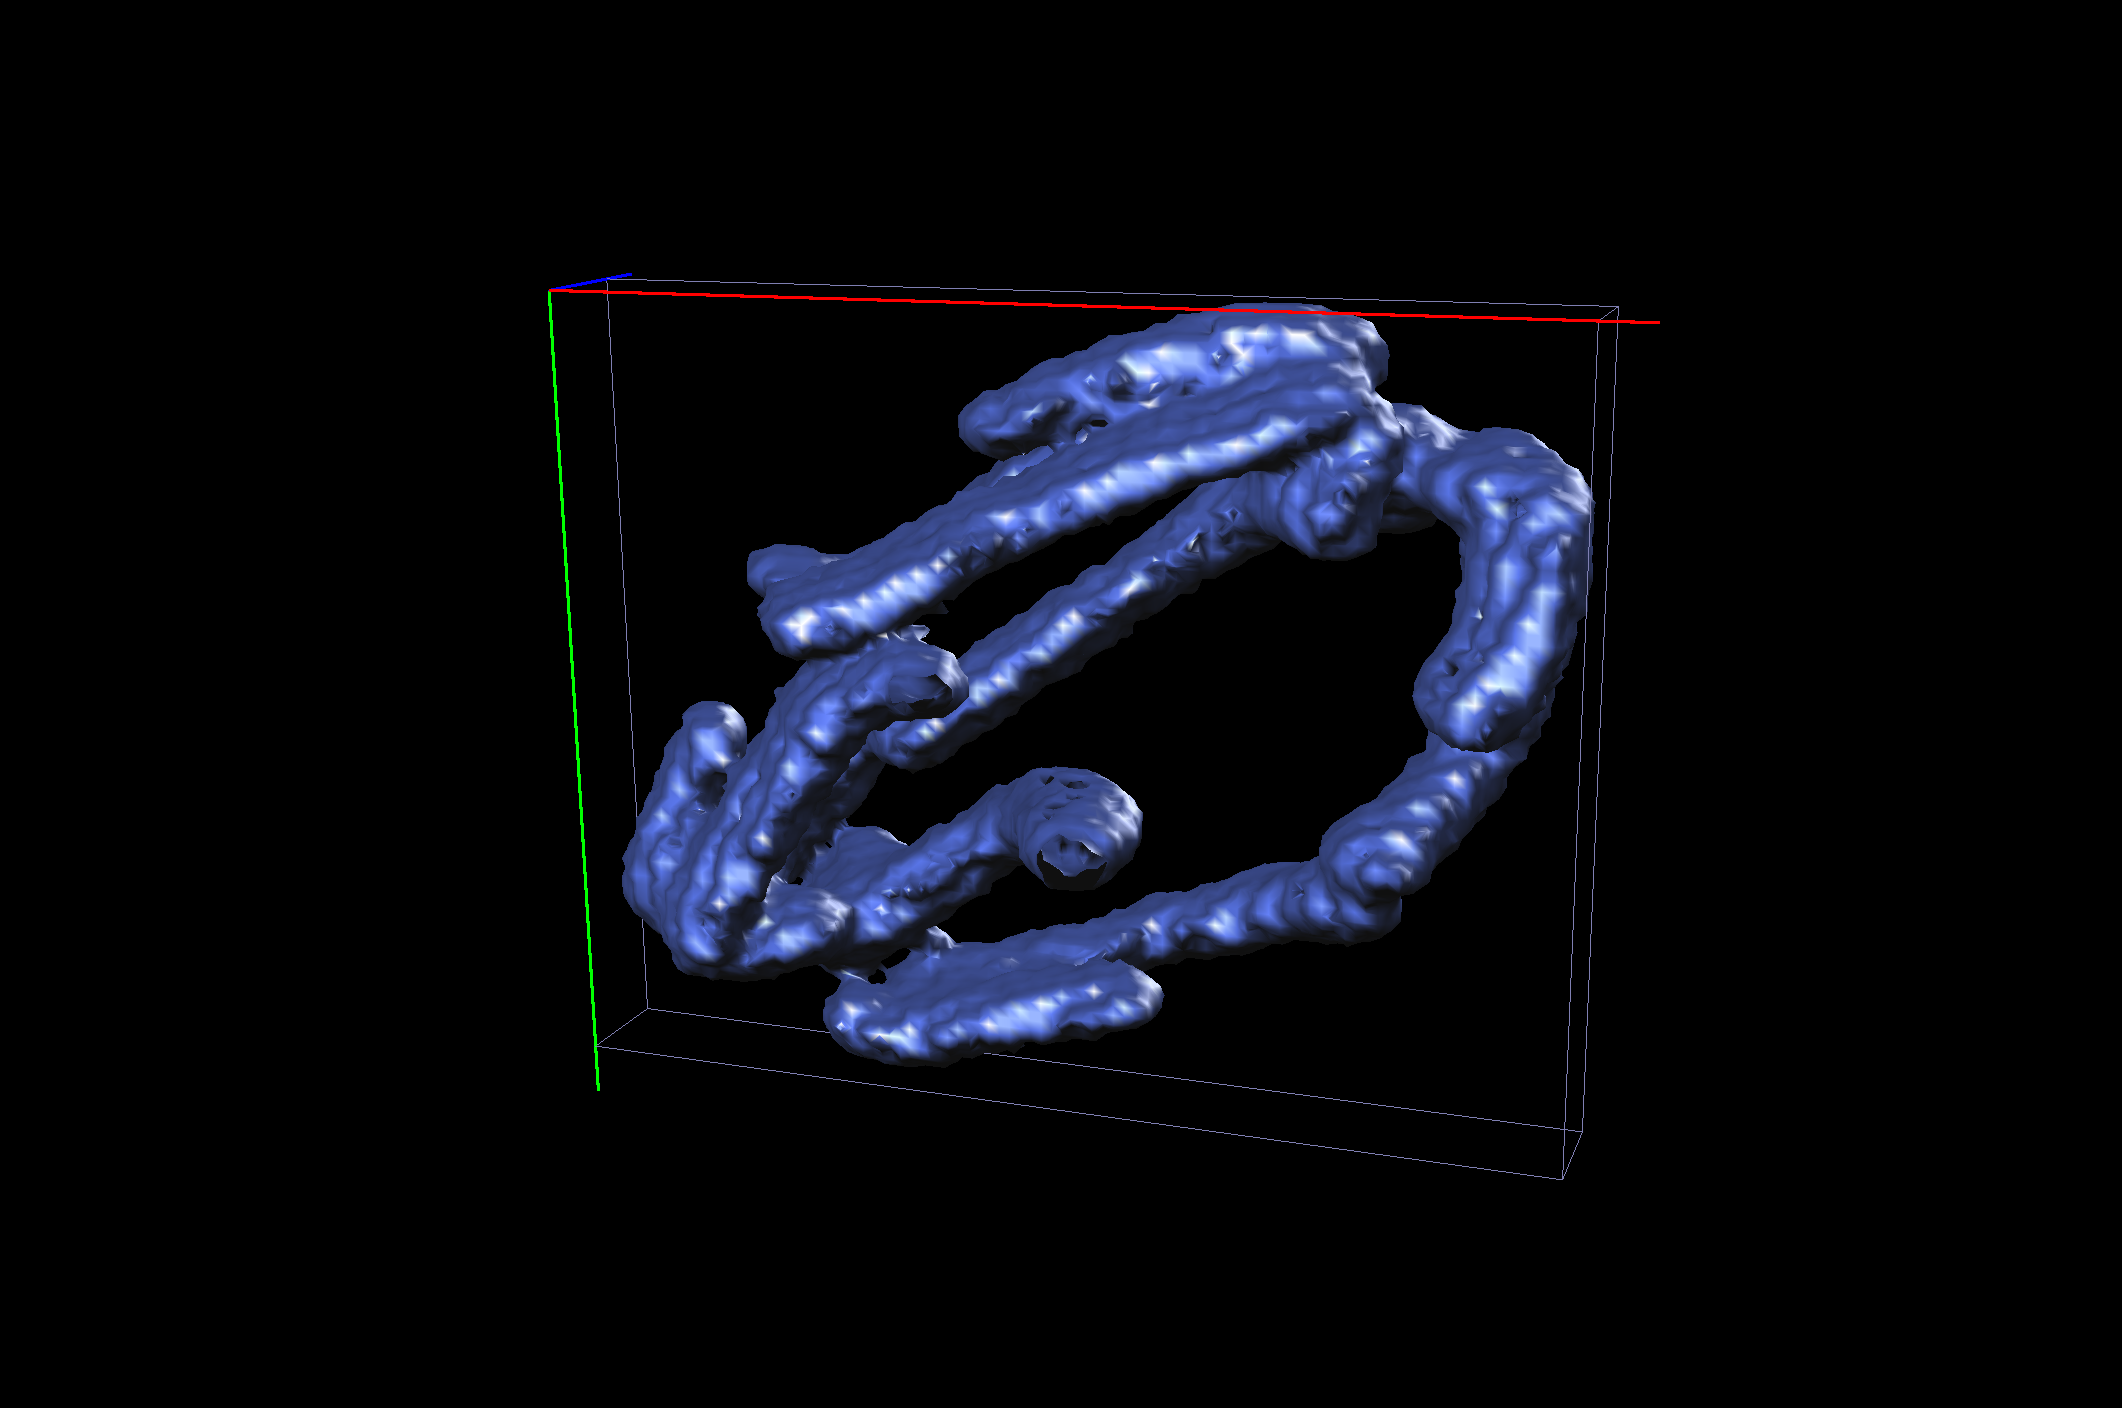
\includegraphics[width=0.3\linewidth]{Report/Images/6.3.2/75-150,100.png}
    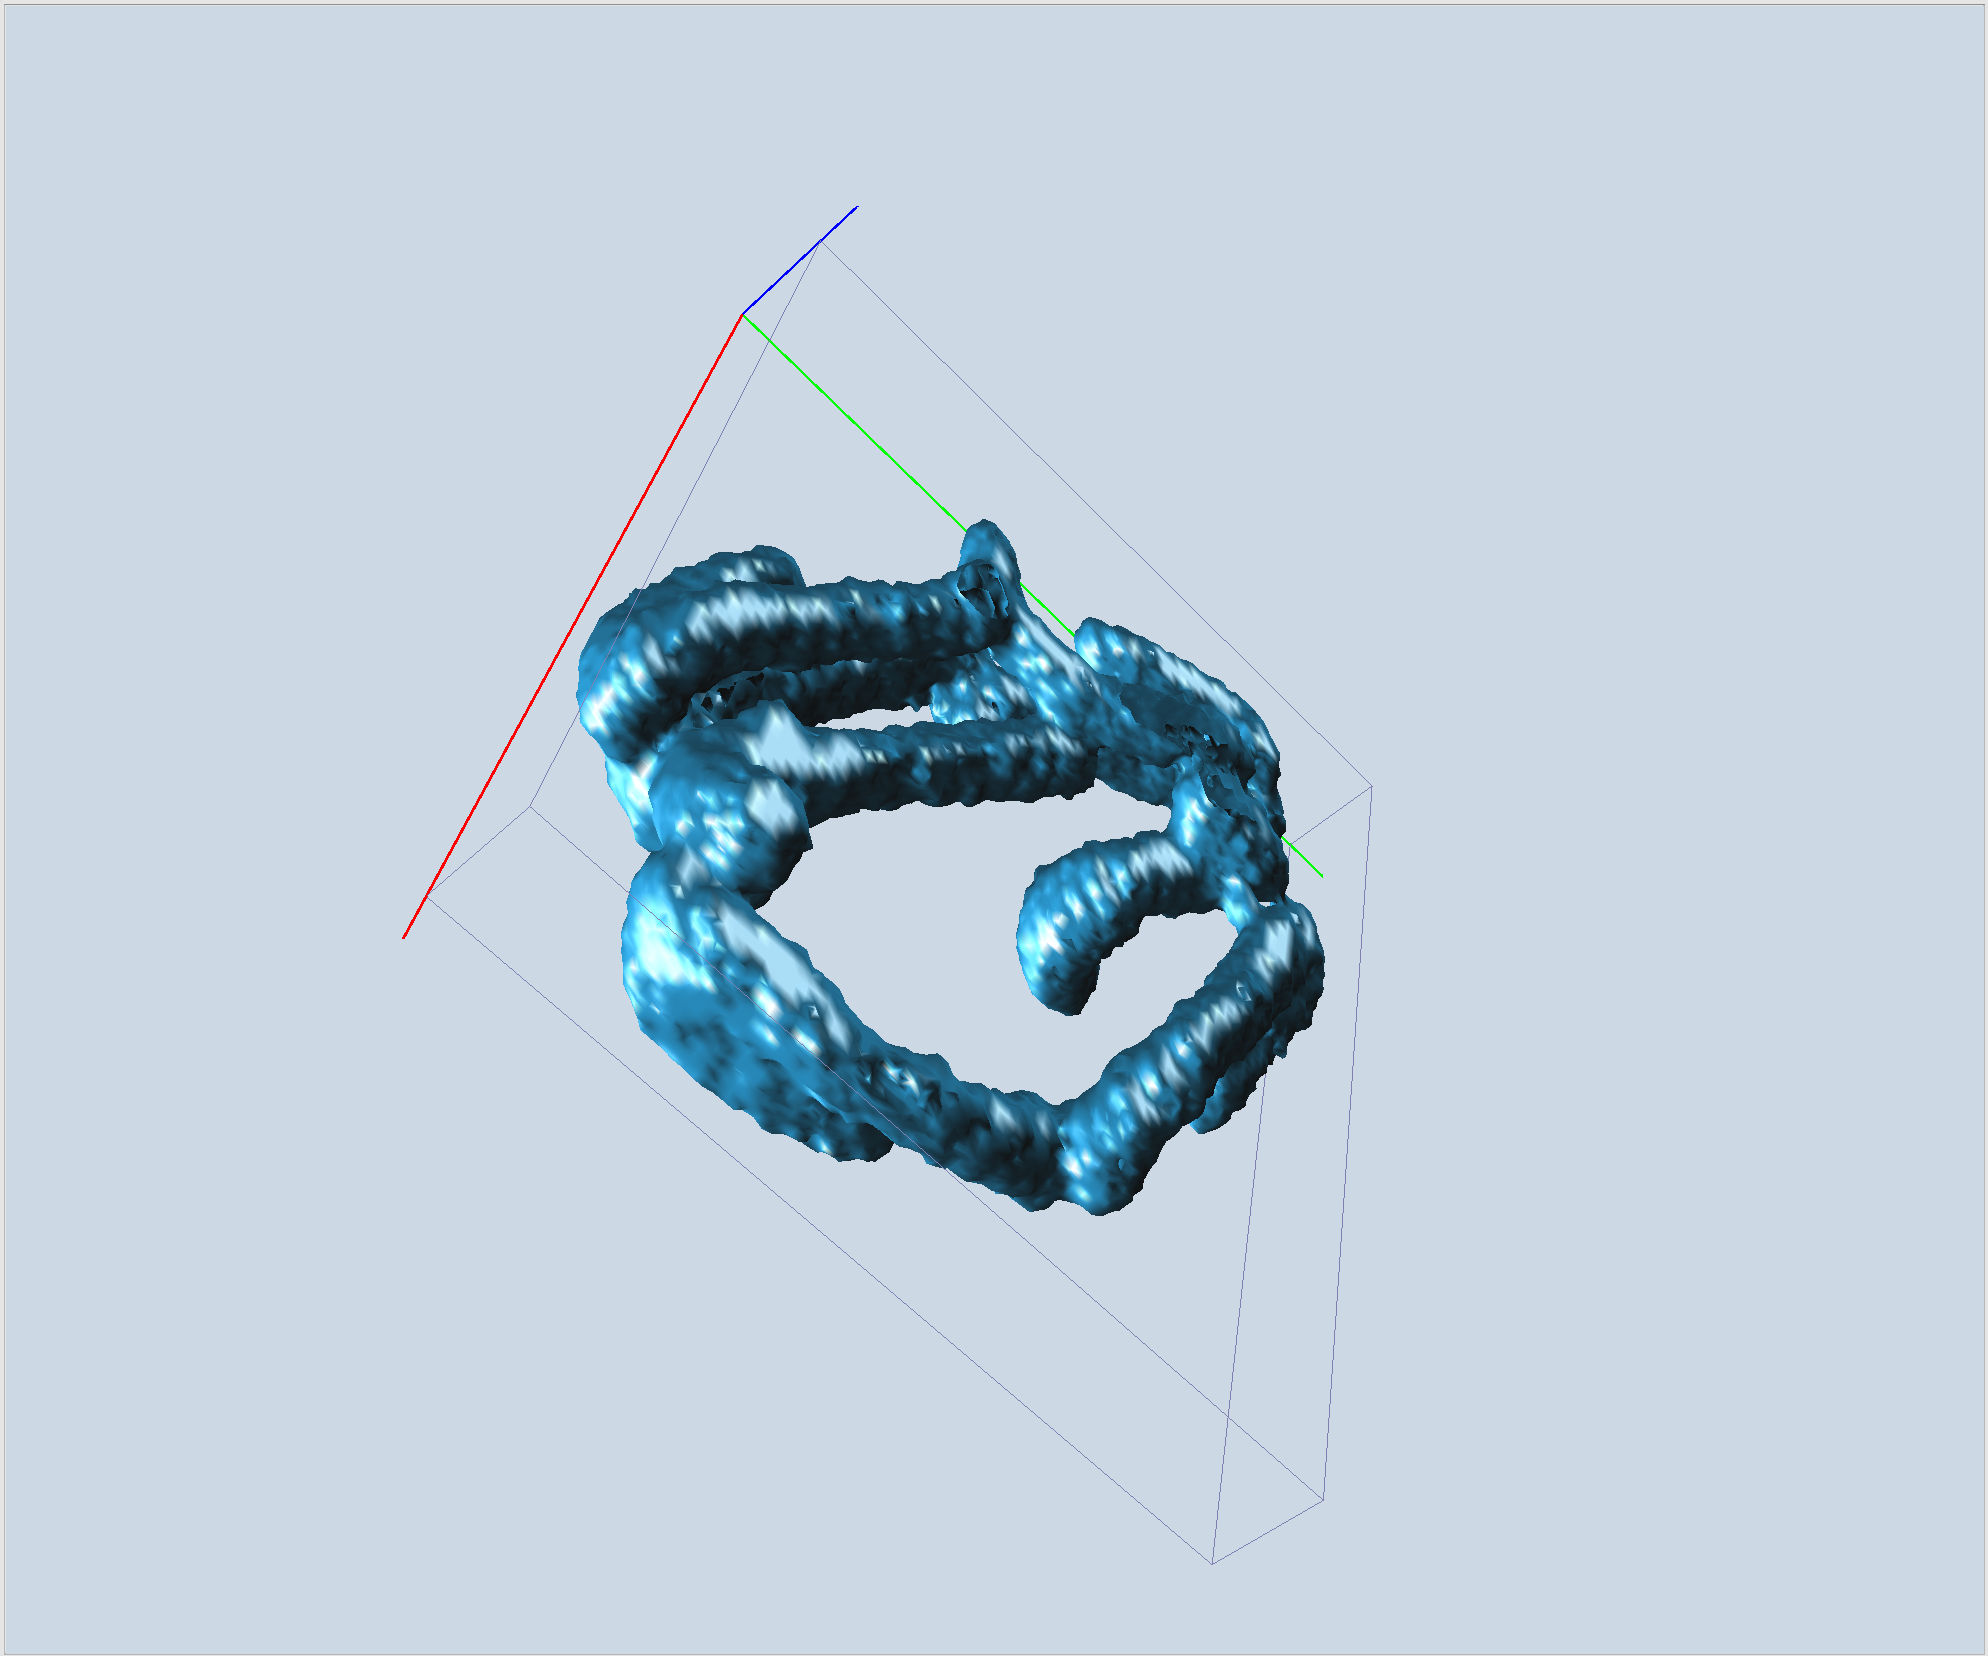
\includegraphics[width=0.3\linewidth]{Report/Images/6.3.2/75-150,100-rotated.png}
    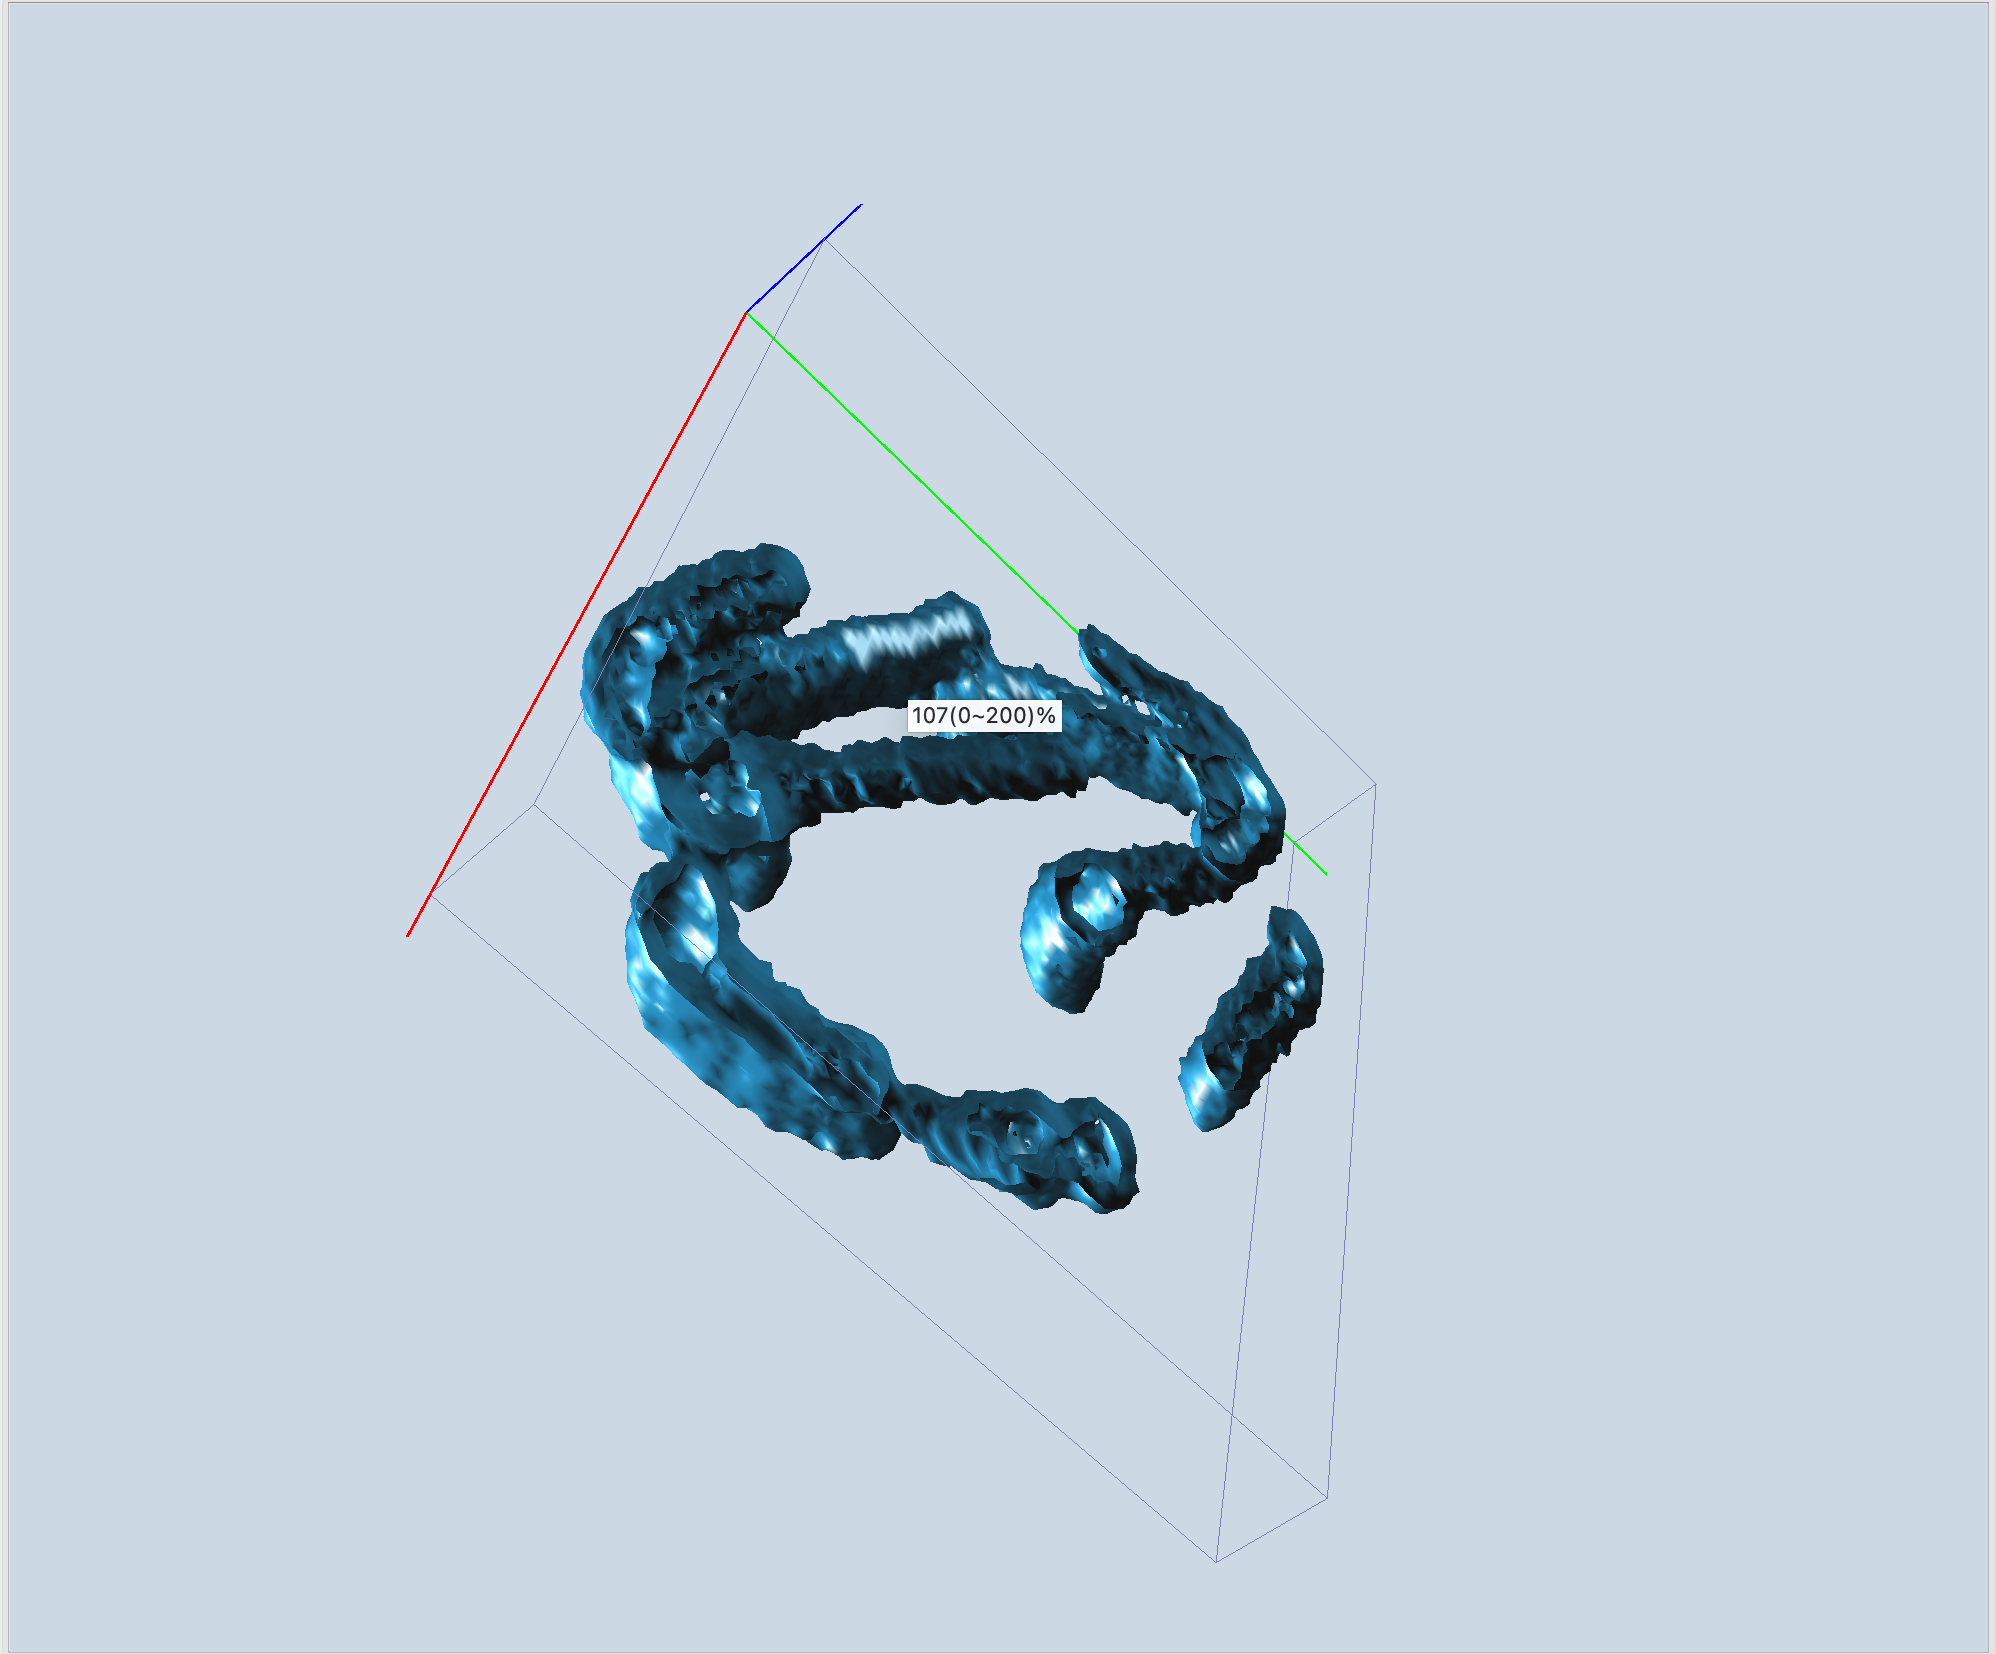
\includegraphics[width=0.3\linewidth]{Report/Images/6.3.2/75-150,100-sliced.png}
    \caption{Threshold: 75-150, mesh density:100, original (left), rotated (middle), cross-section(right)}
    \label{fig:surface_vis_75_150-100}
\end{figure}


\begin{figure}[h!]
    \centering
    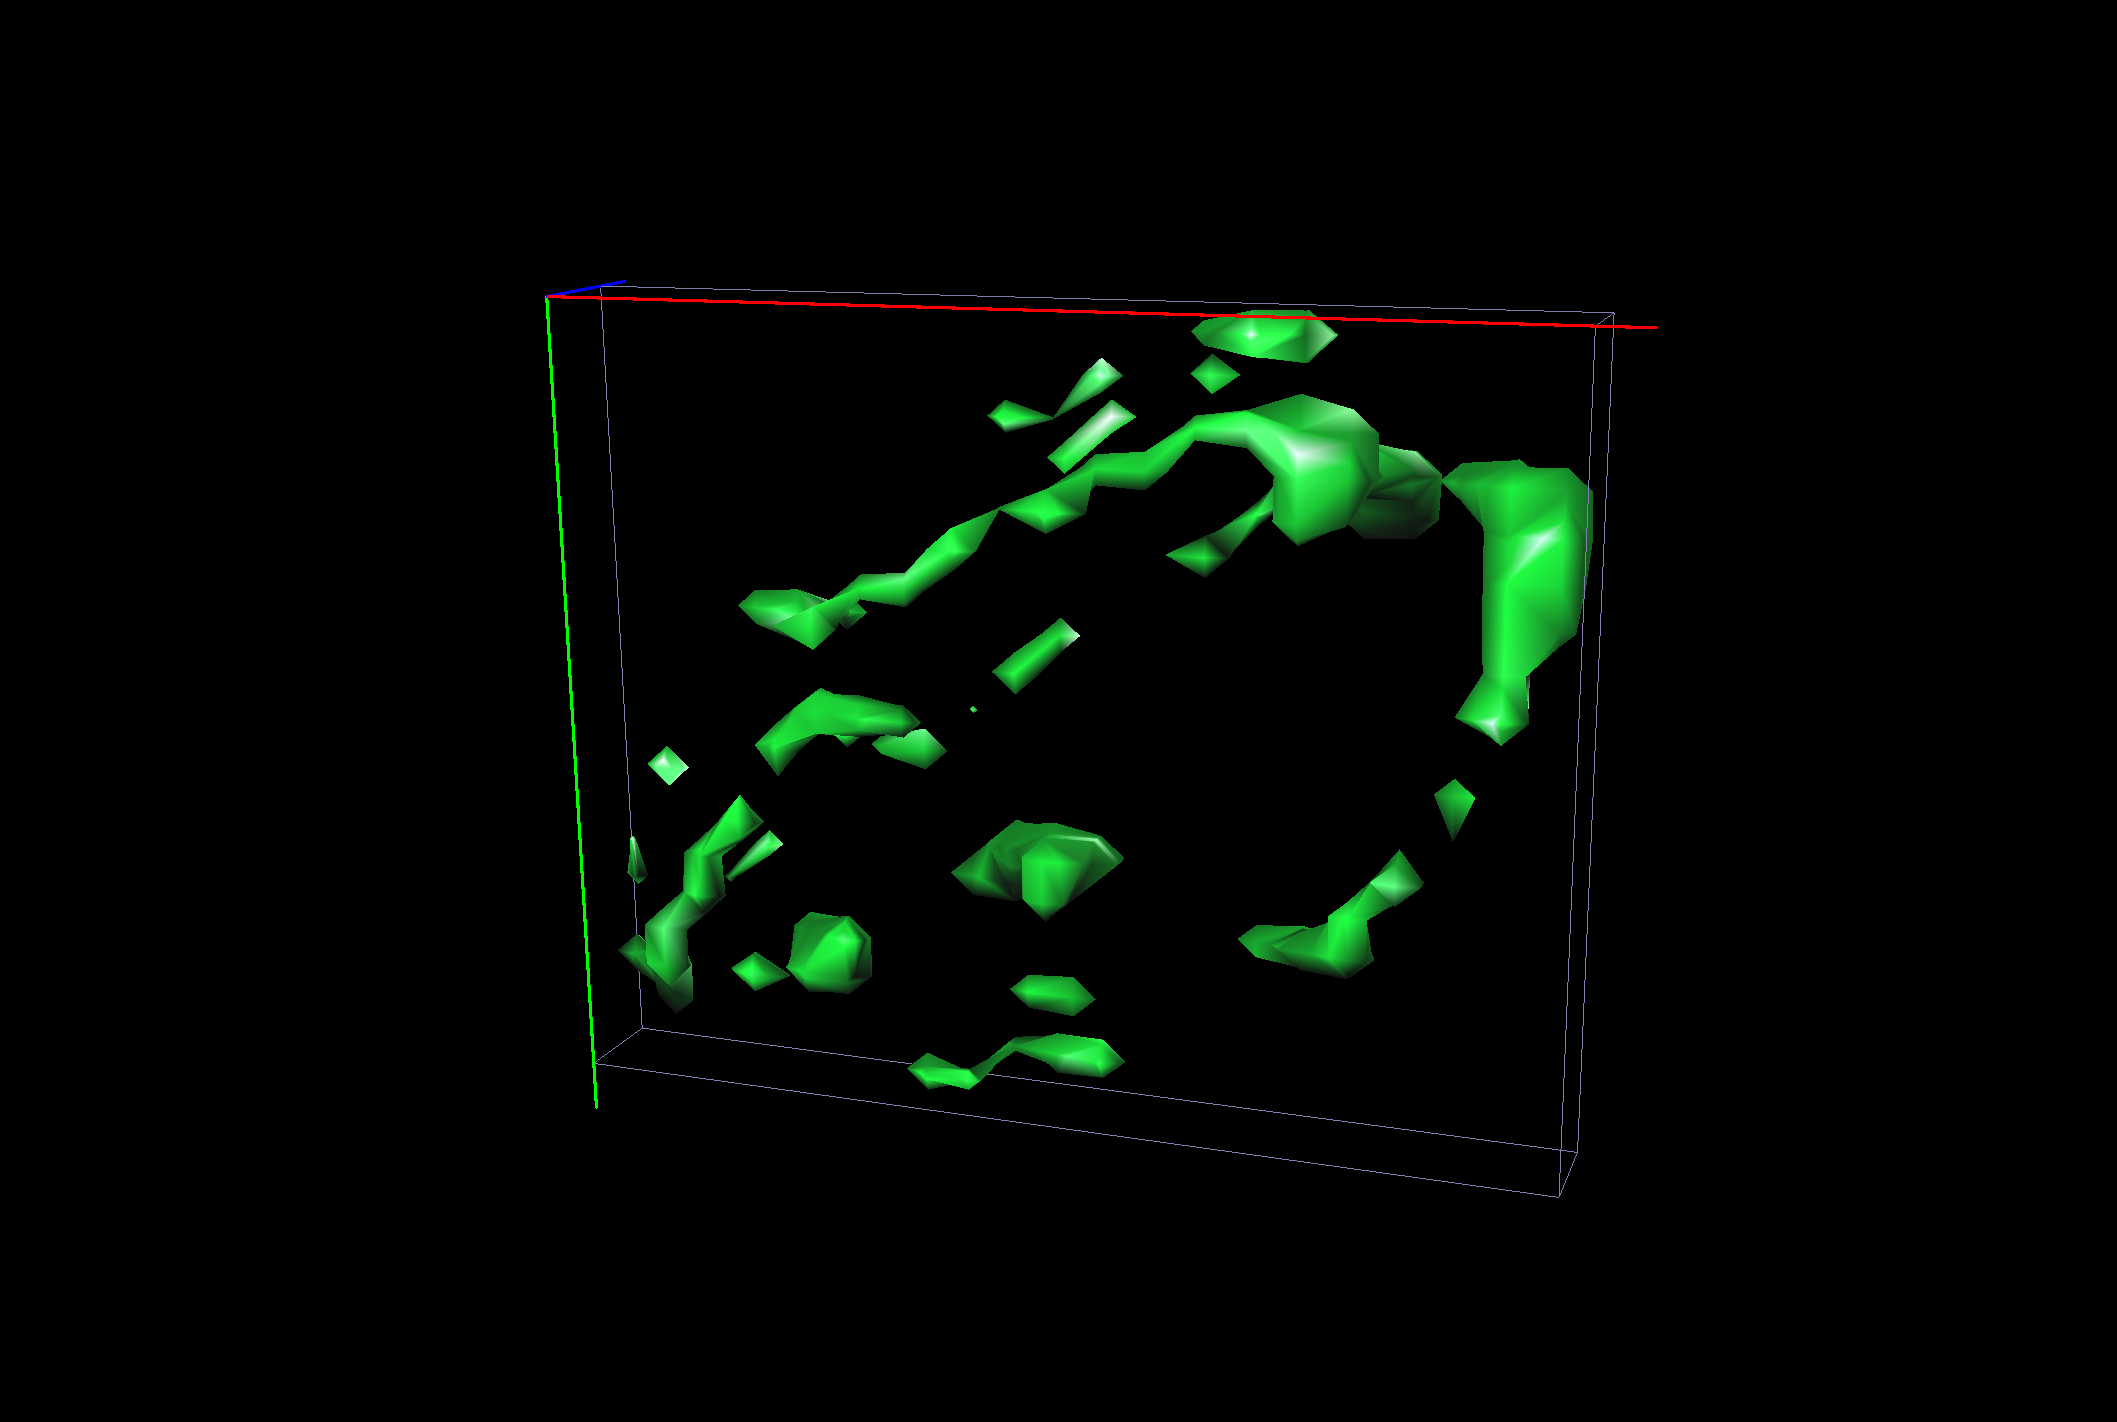
\includegraphics[width=0.3\linewidth]{Report/Images/6.3.2/150-255,25.png}
    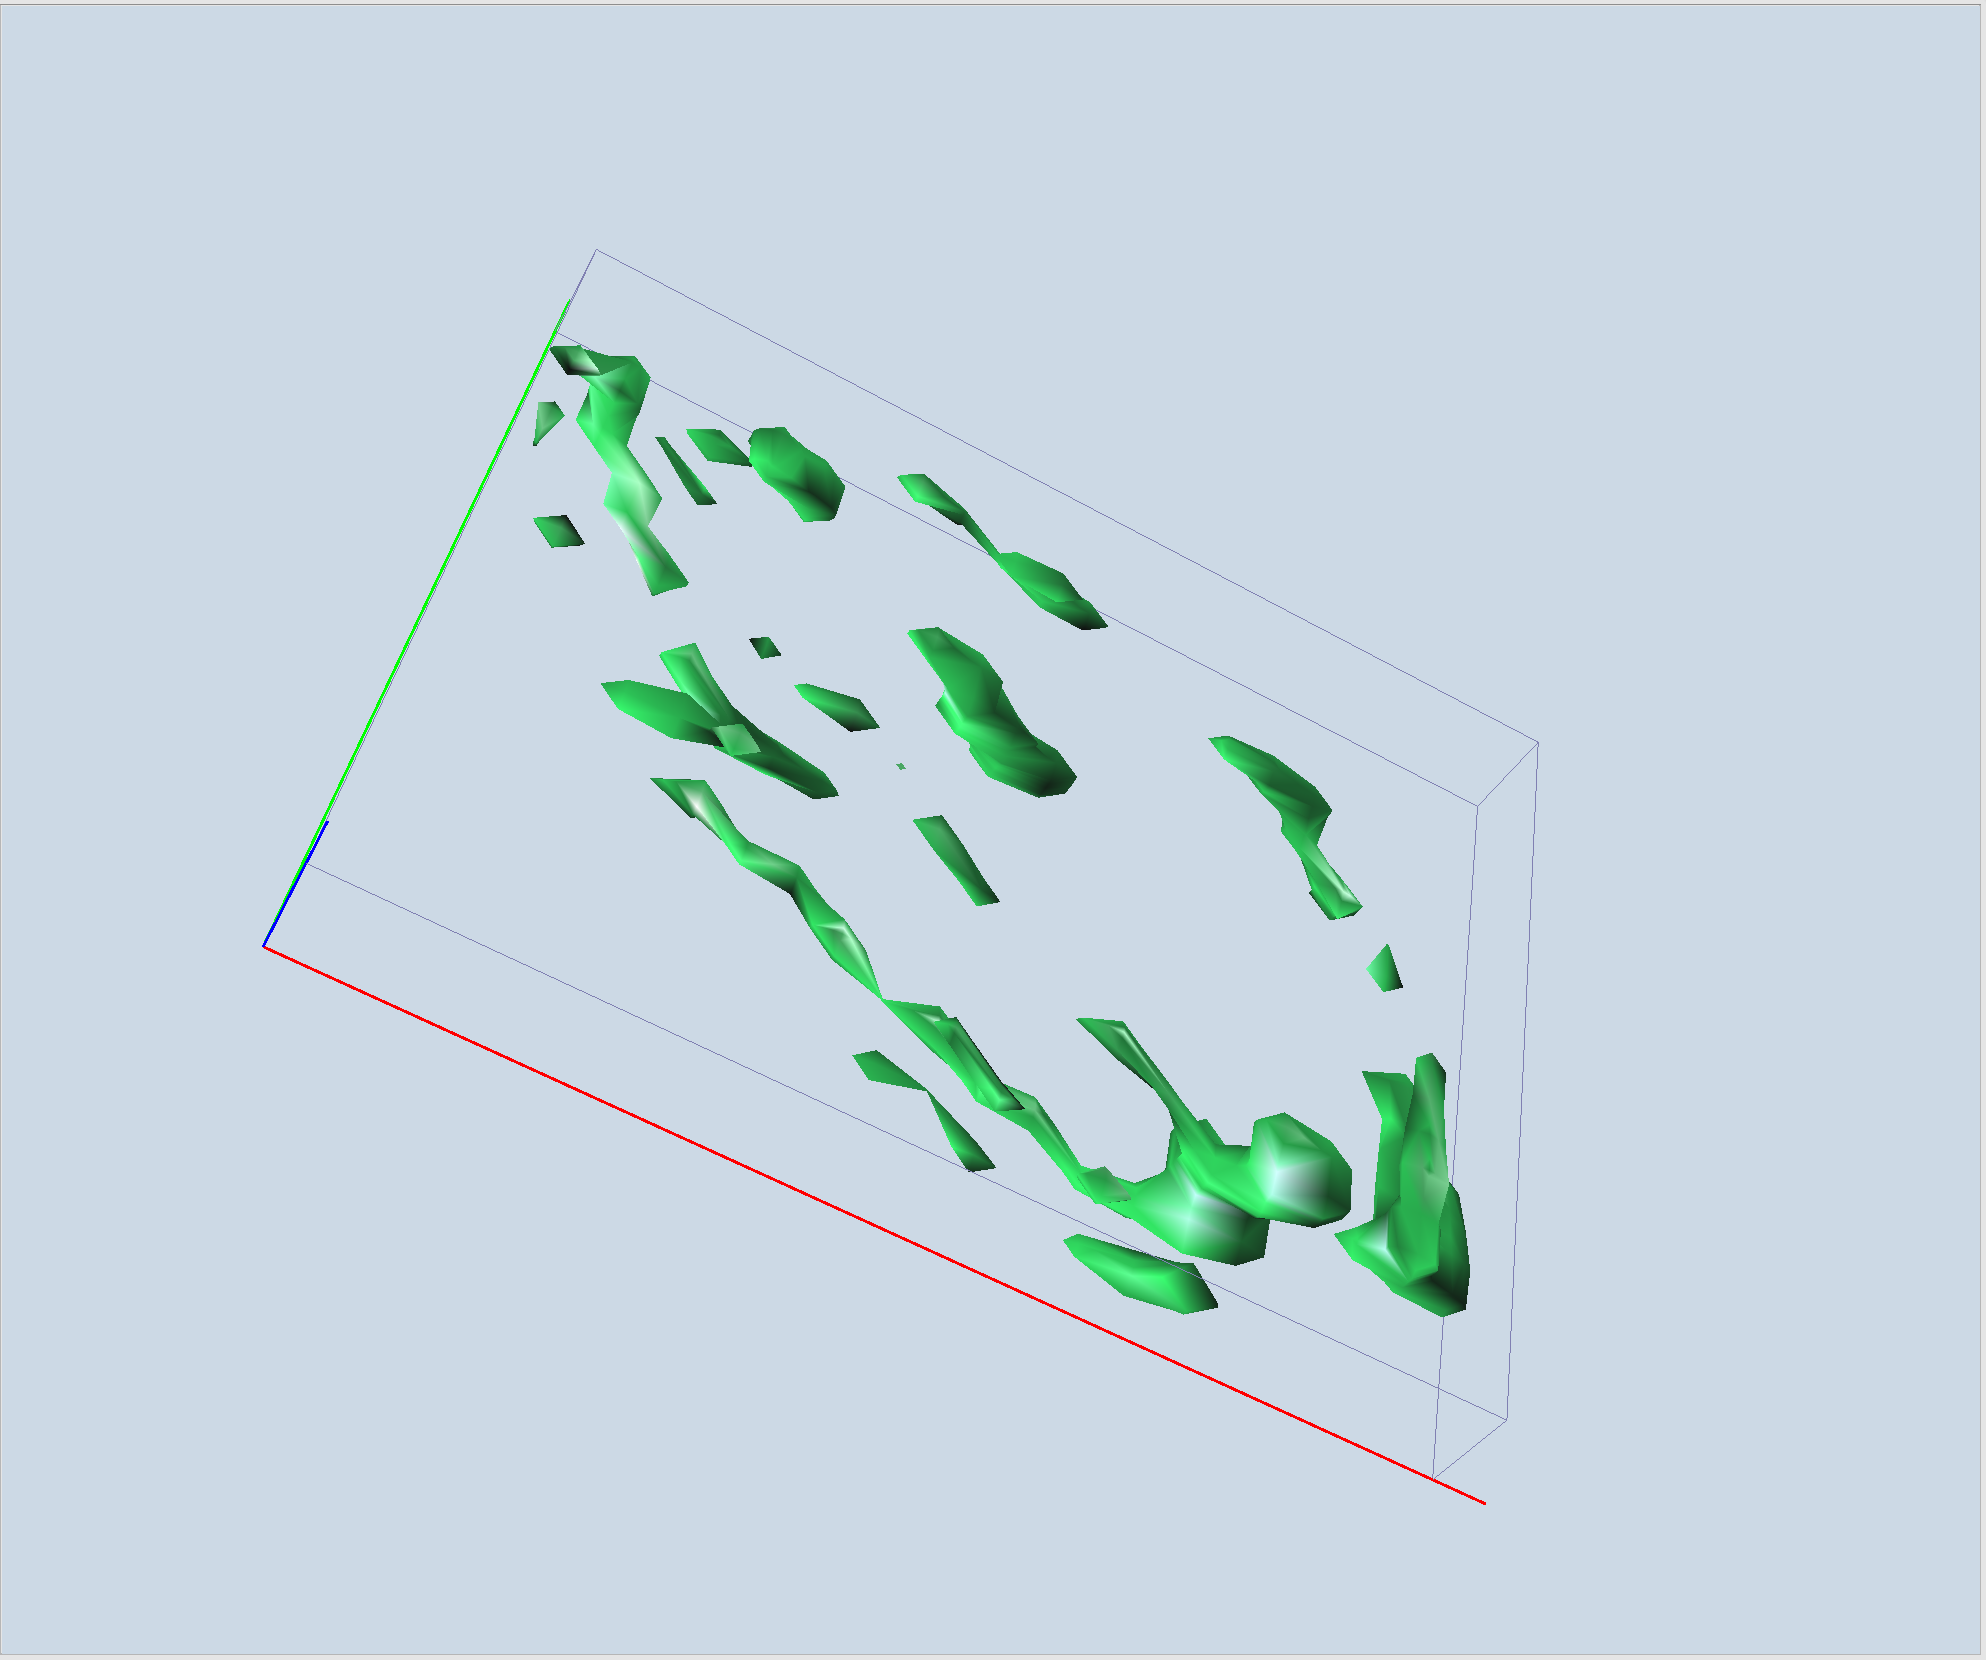
\includegraphics[width=0.3\linewidth]{Report/Images/6.3.2/150-255,25-rotated.png}
    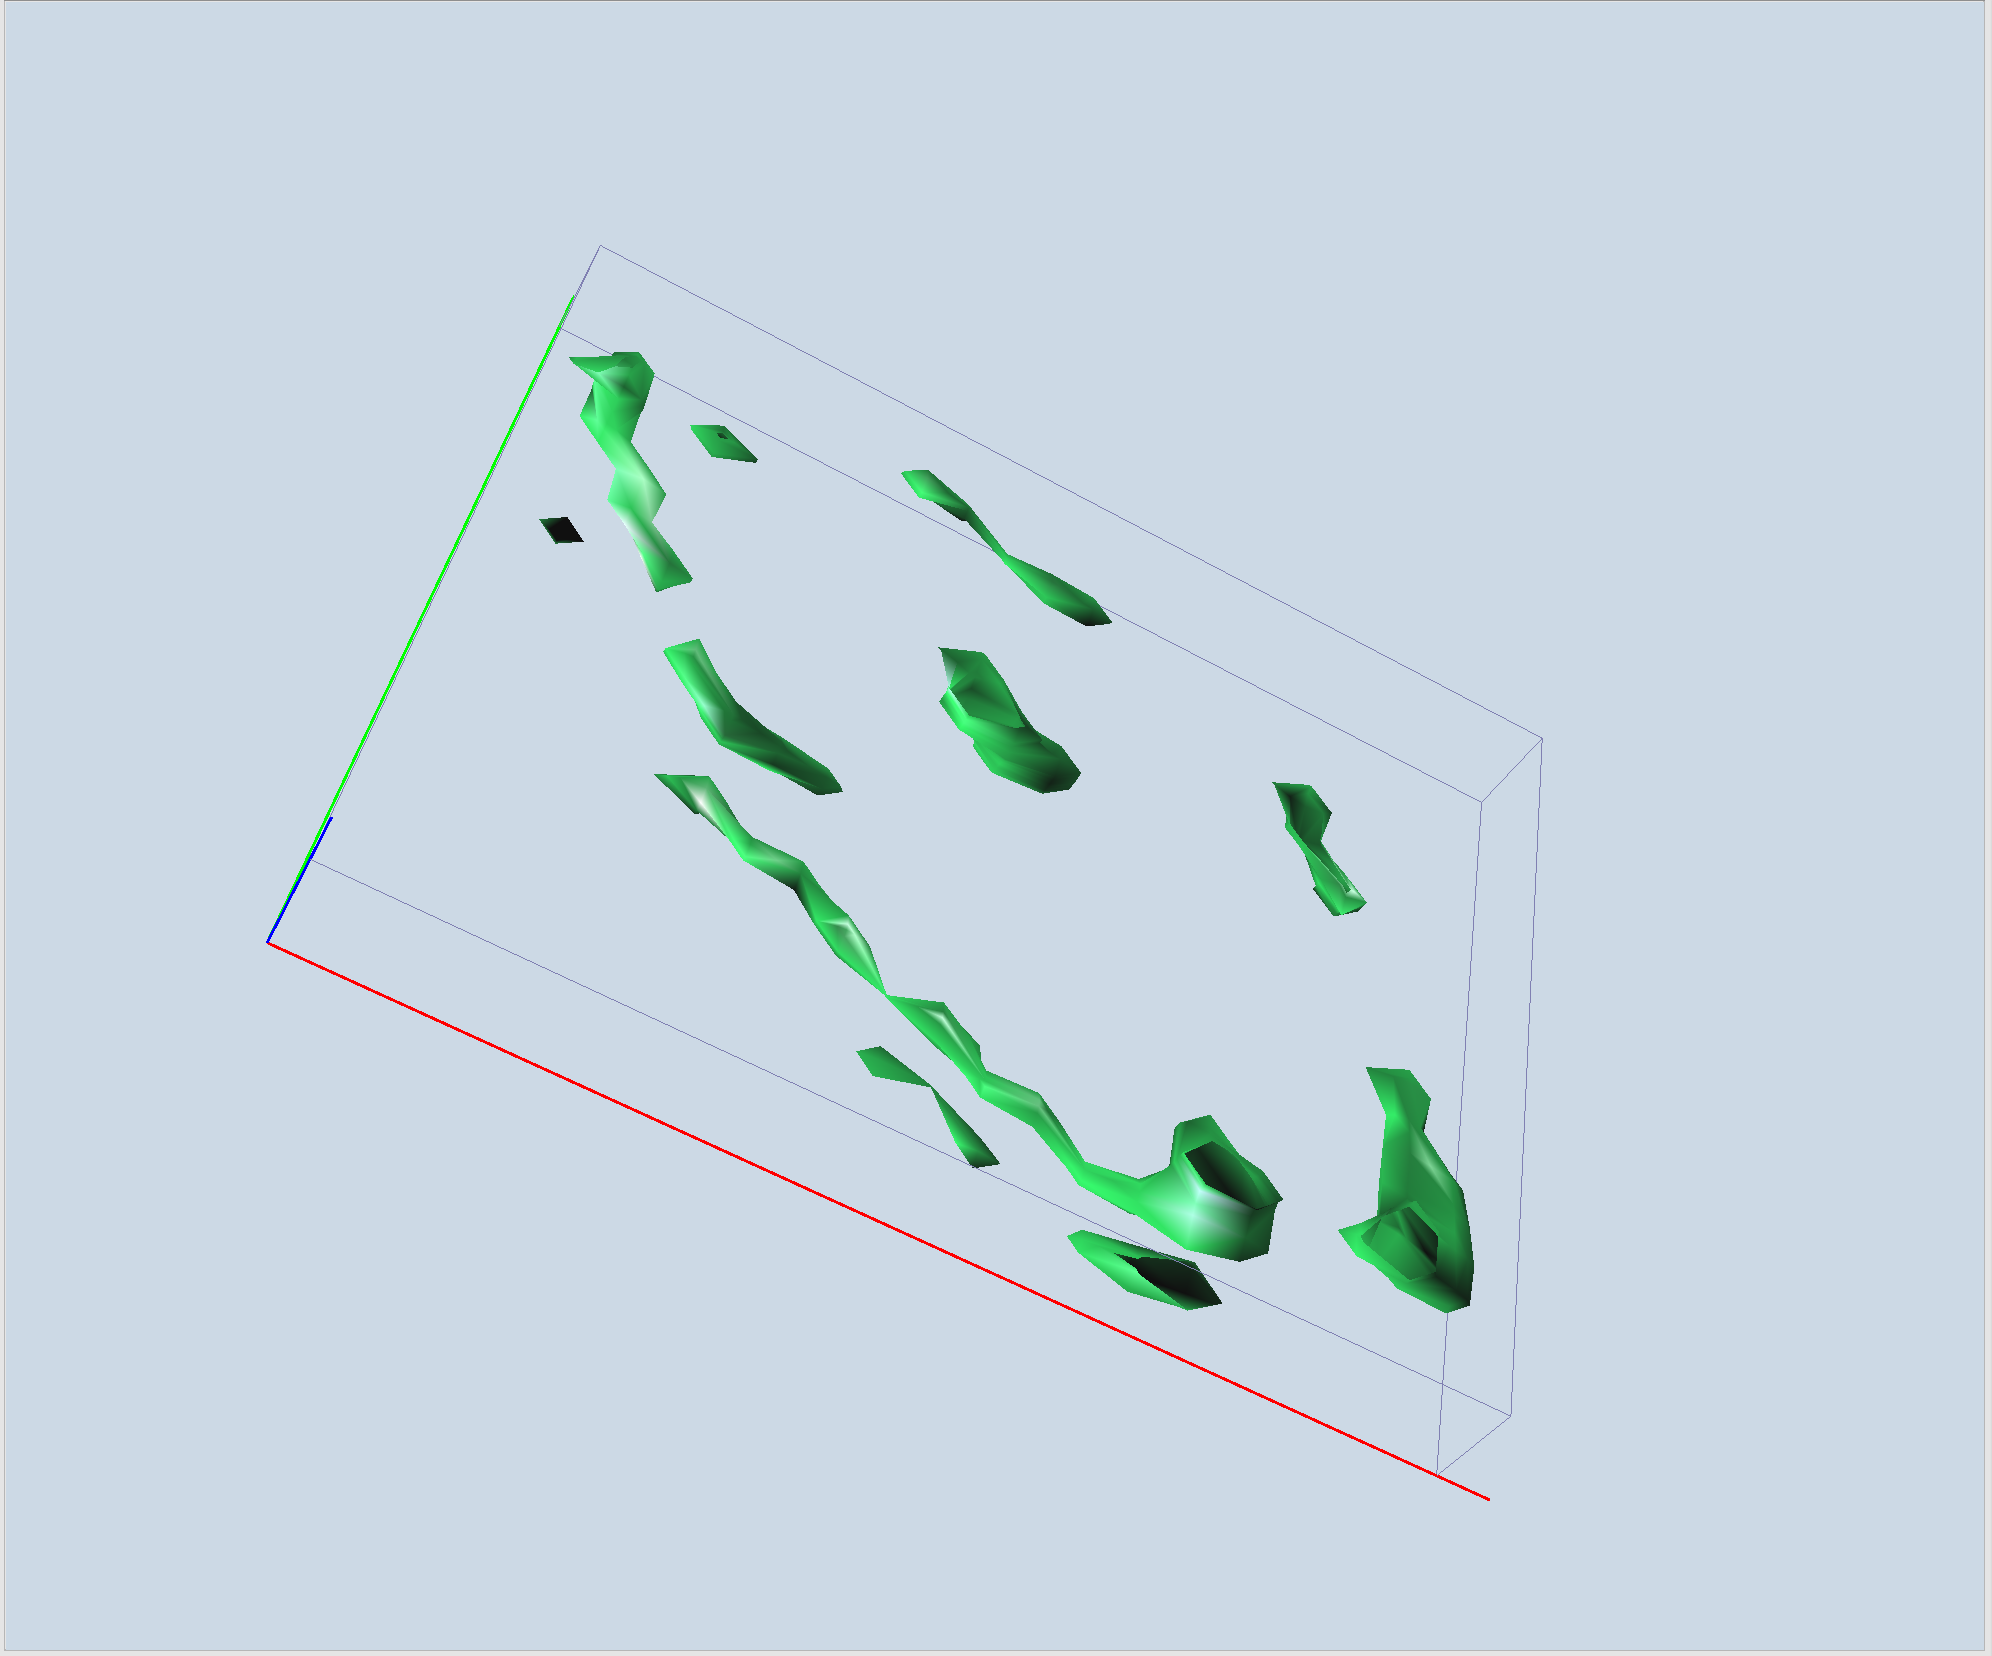
\includegraphics[width=0.3\linewidth]{Report/Images/6.3.2/150-255,25-sliced.png}
    \caption{Threshold: 150-255, mesh density:25, original (left), rotated (middle), cross-section(right)}
    \label{fig:surface_vis_150_255-25}
\end{figure}

\begin{figure}[h!]
    \centering
    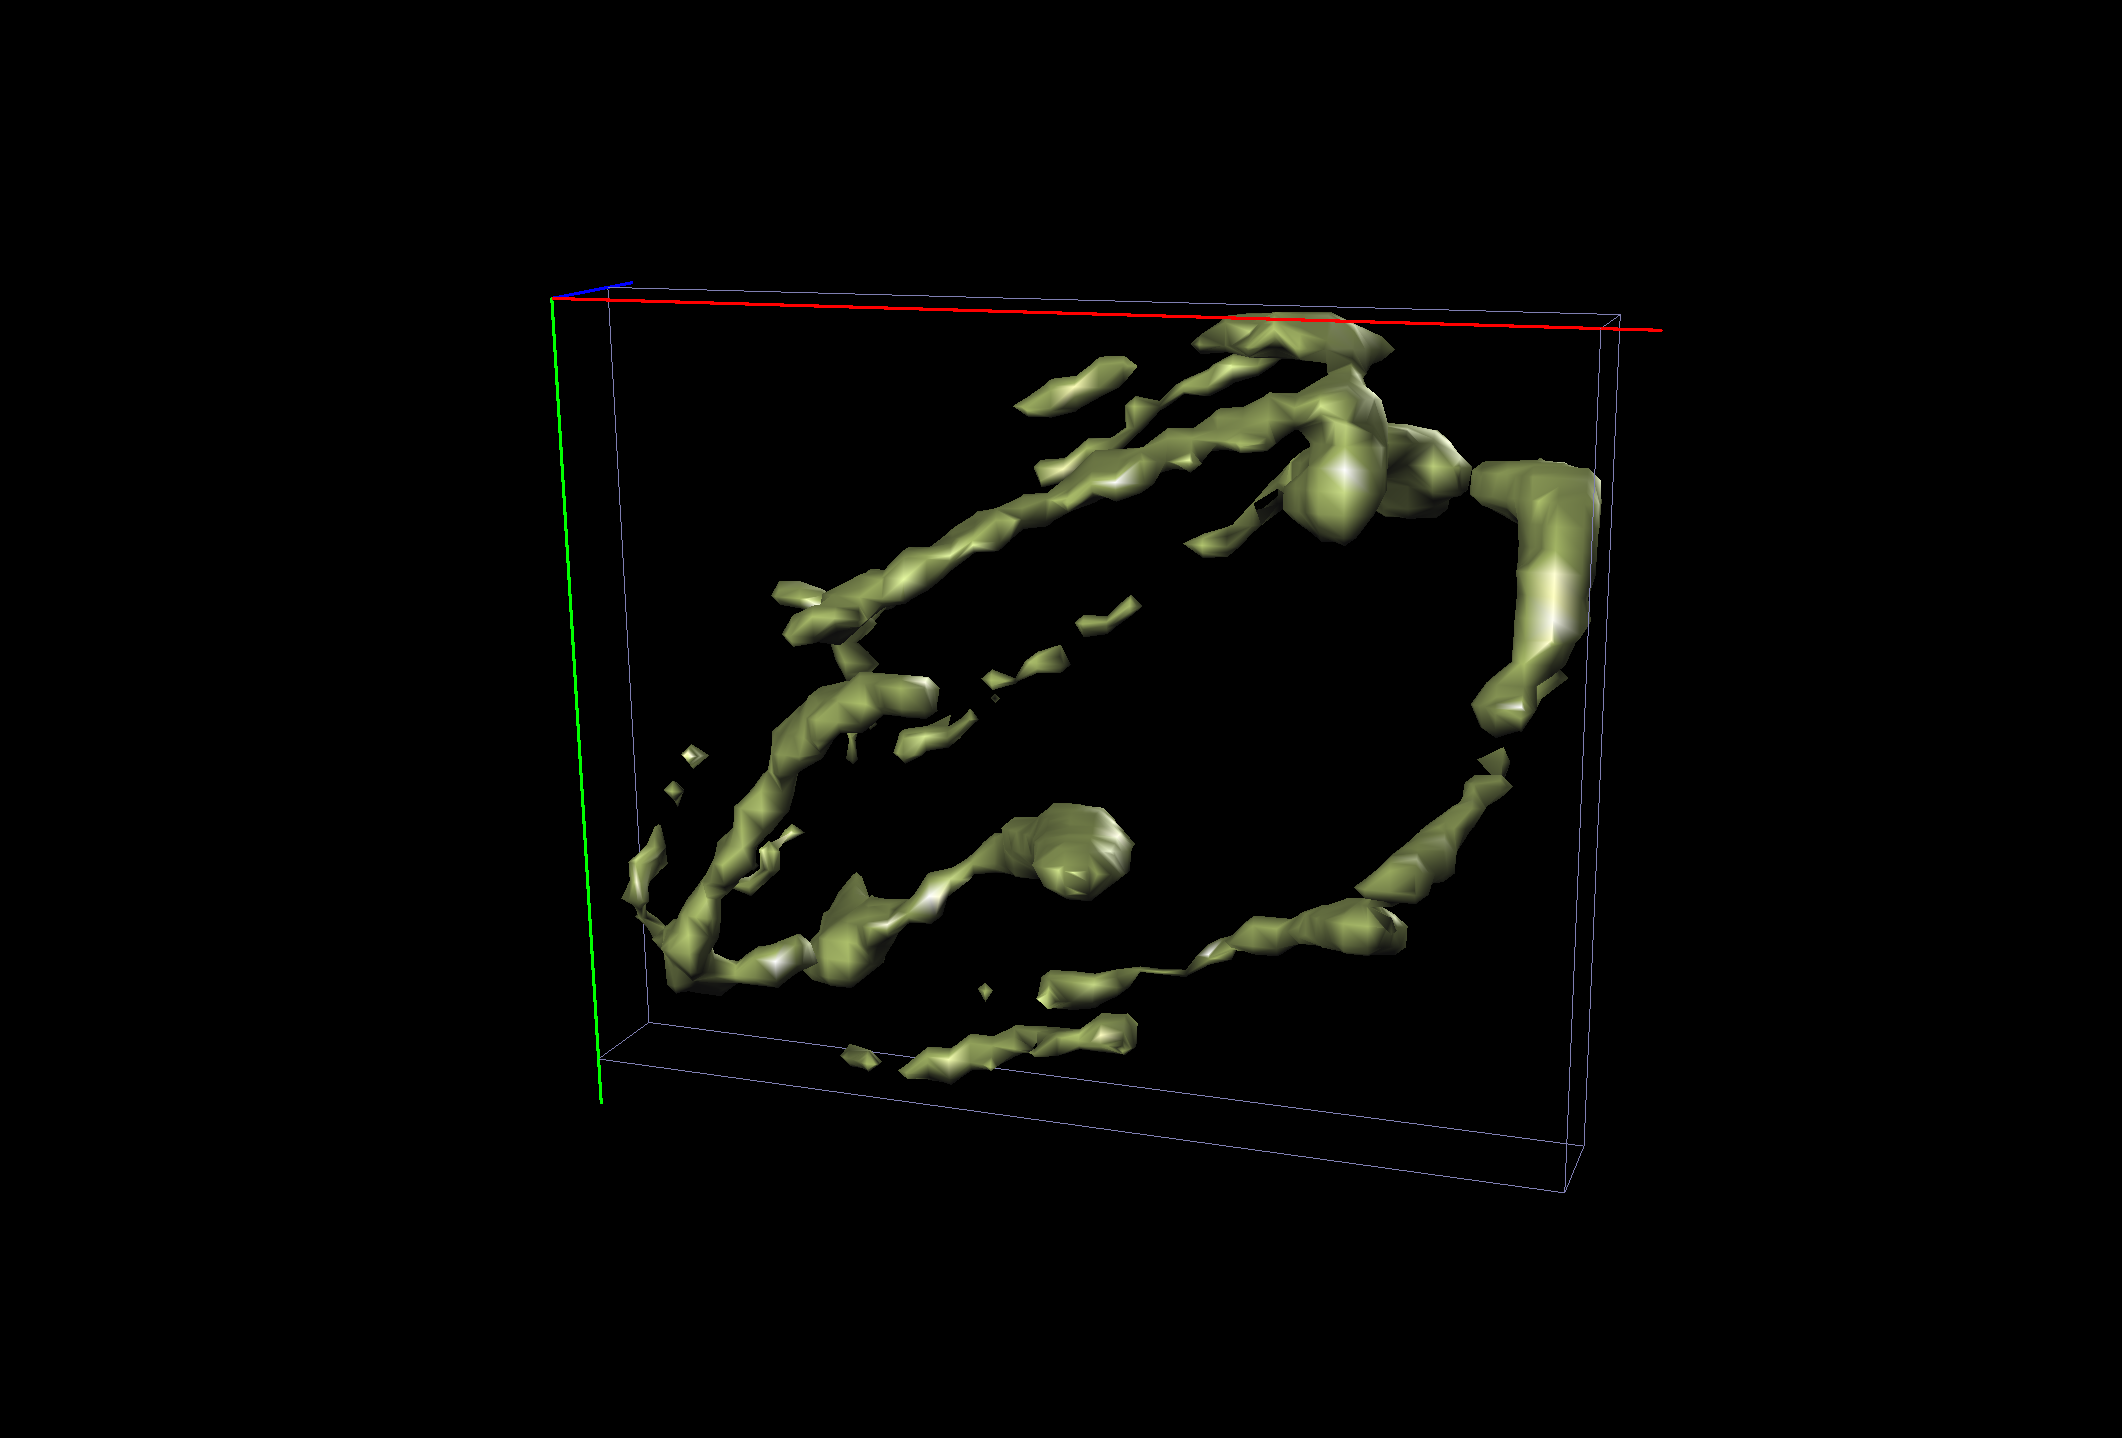
\includegraphics[width=0.3\linewidth]{Report/Images/6.3.2/150-255,50.png}
    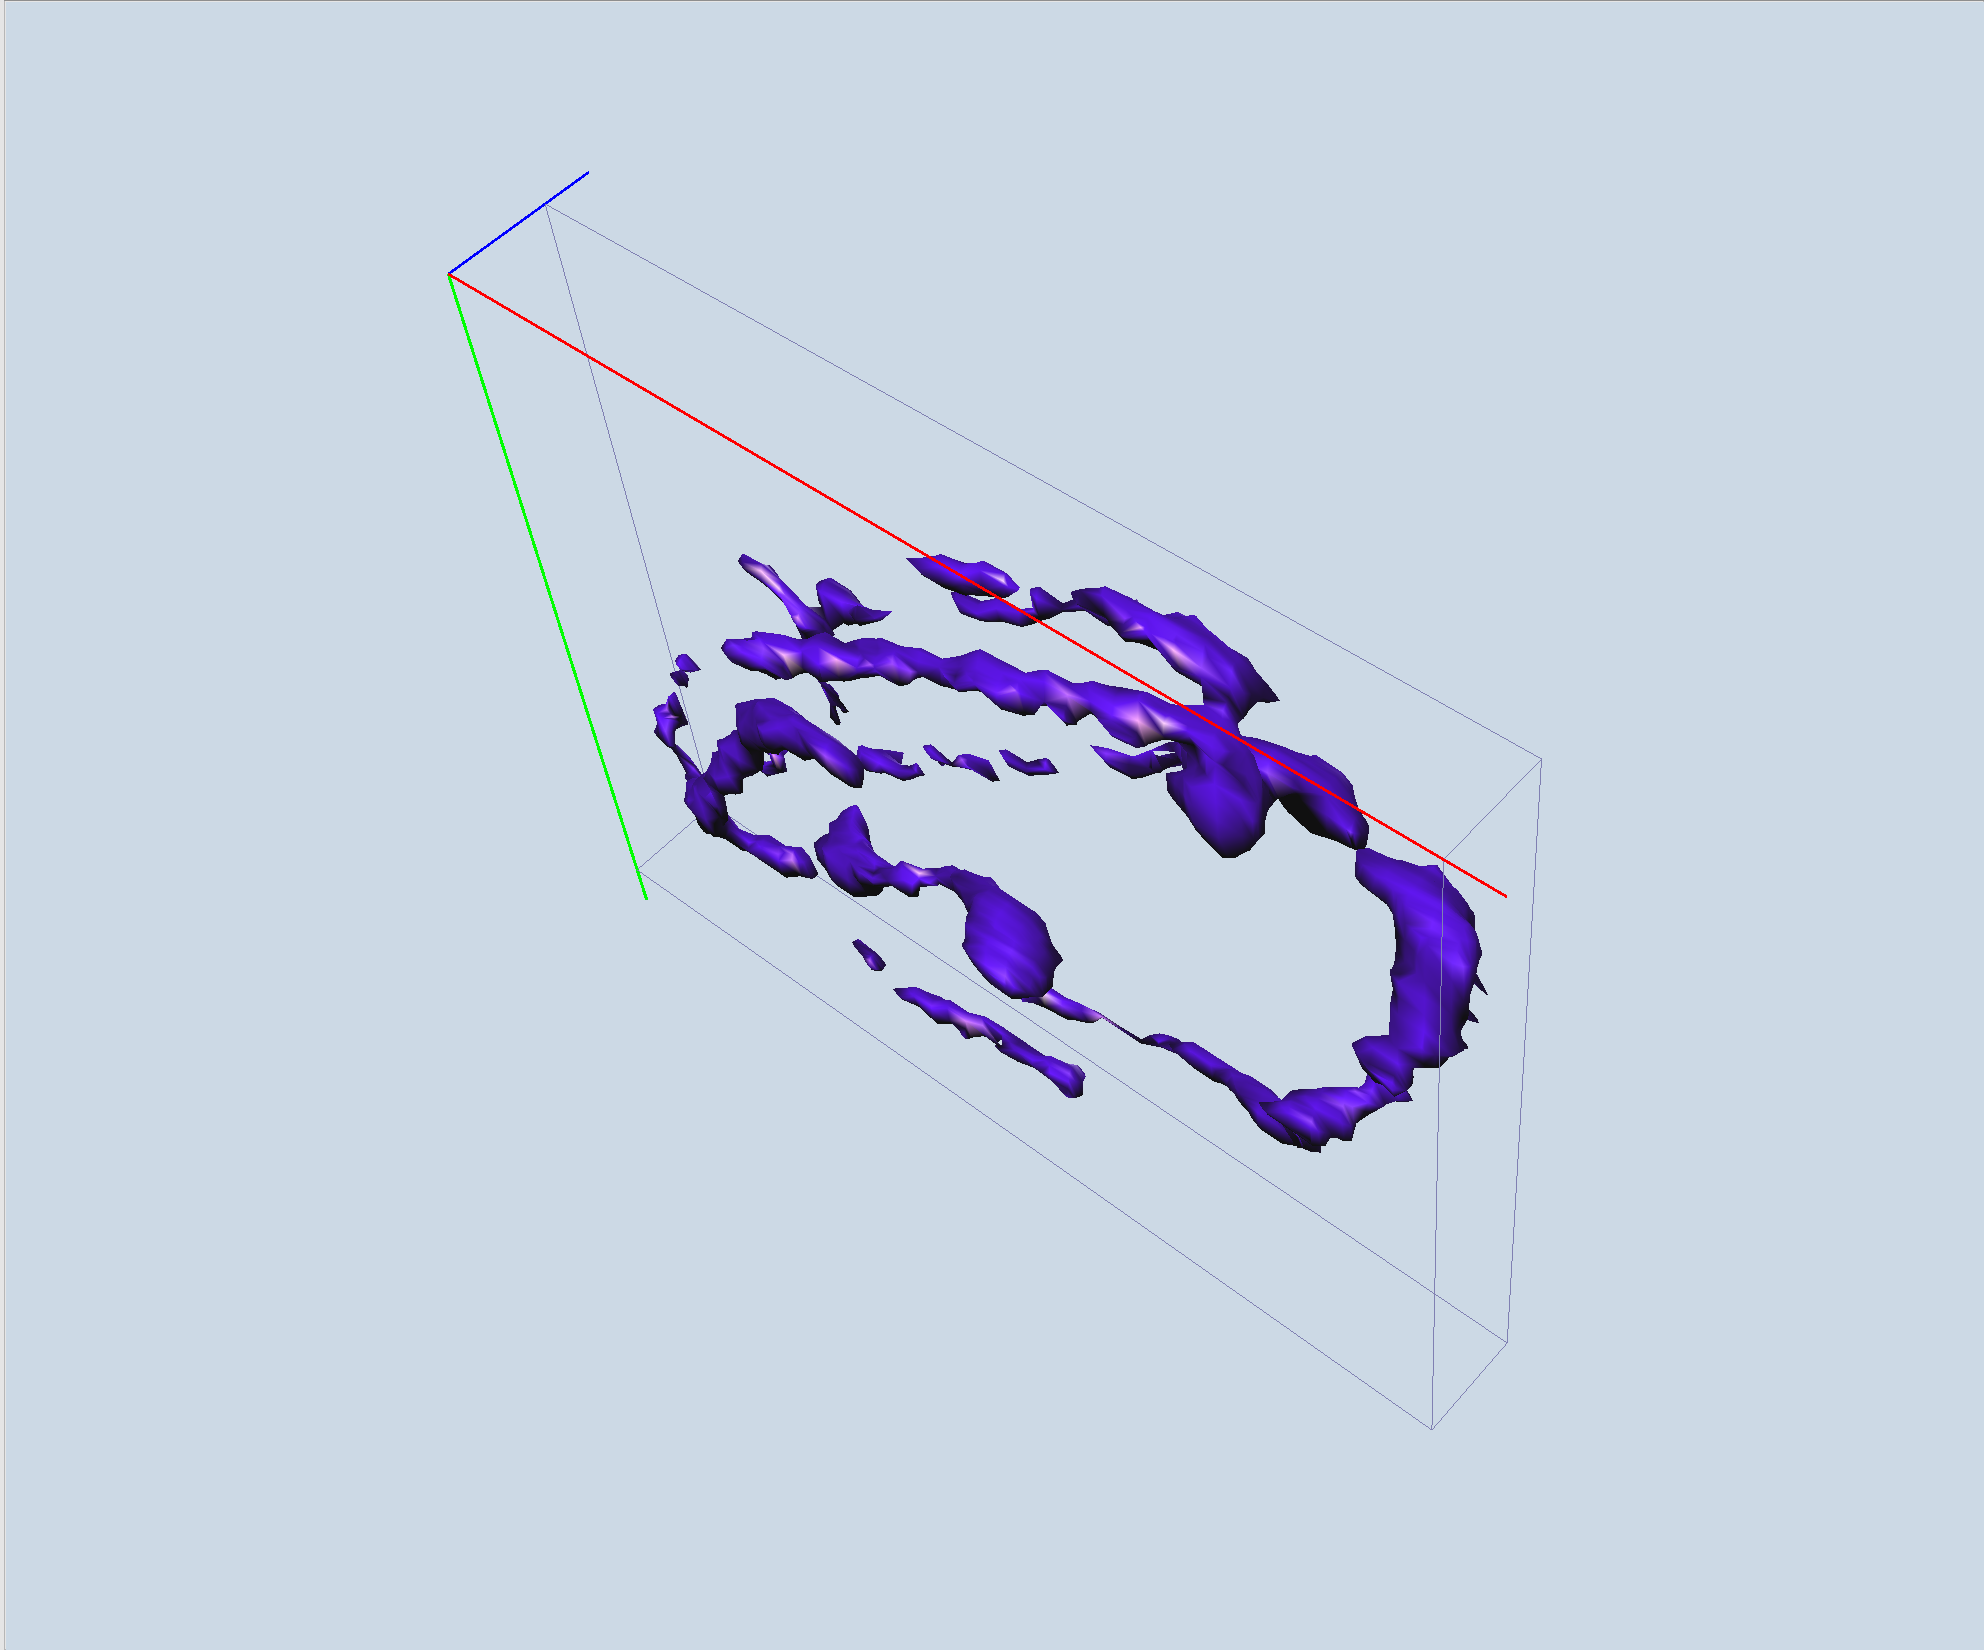
\includegraphics[width=0.3\linewidth]{Report/Images/6.3.2/150-255,50-rotated.png}
    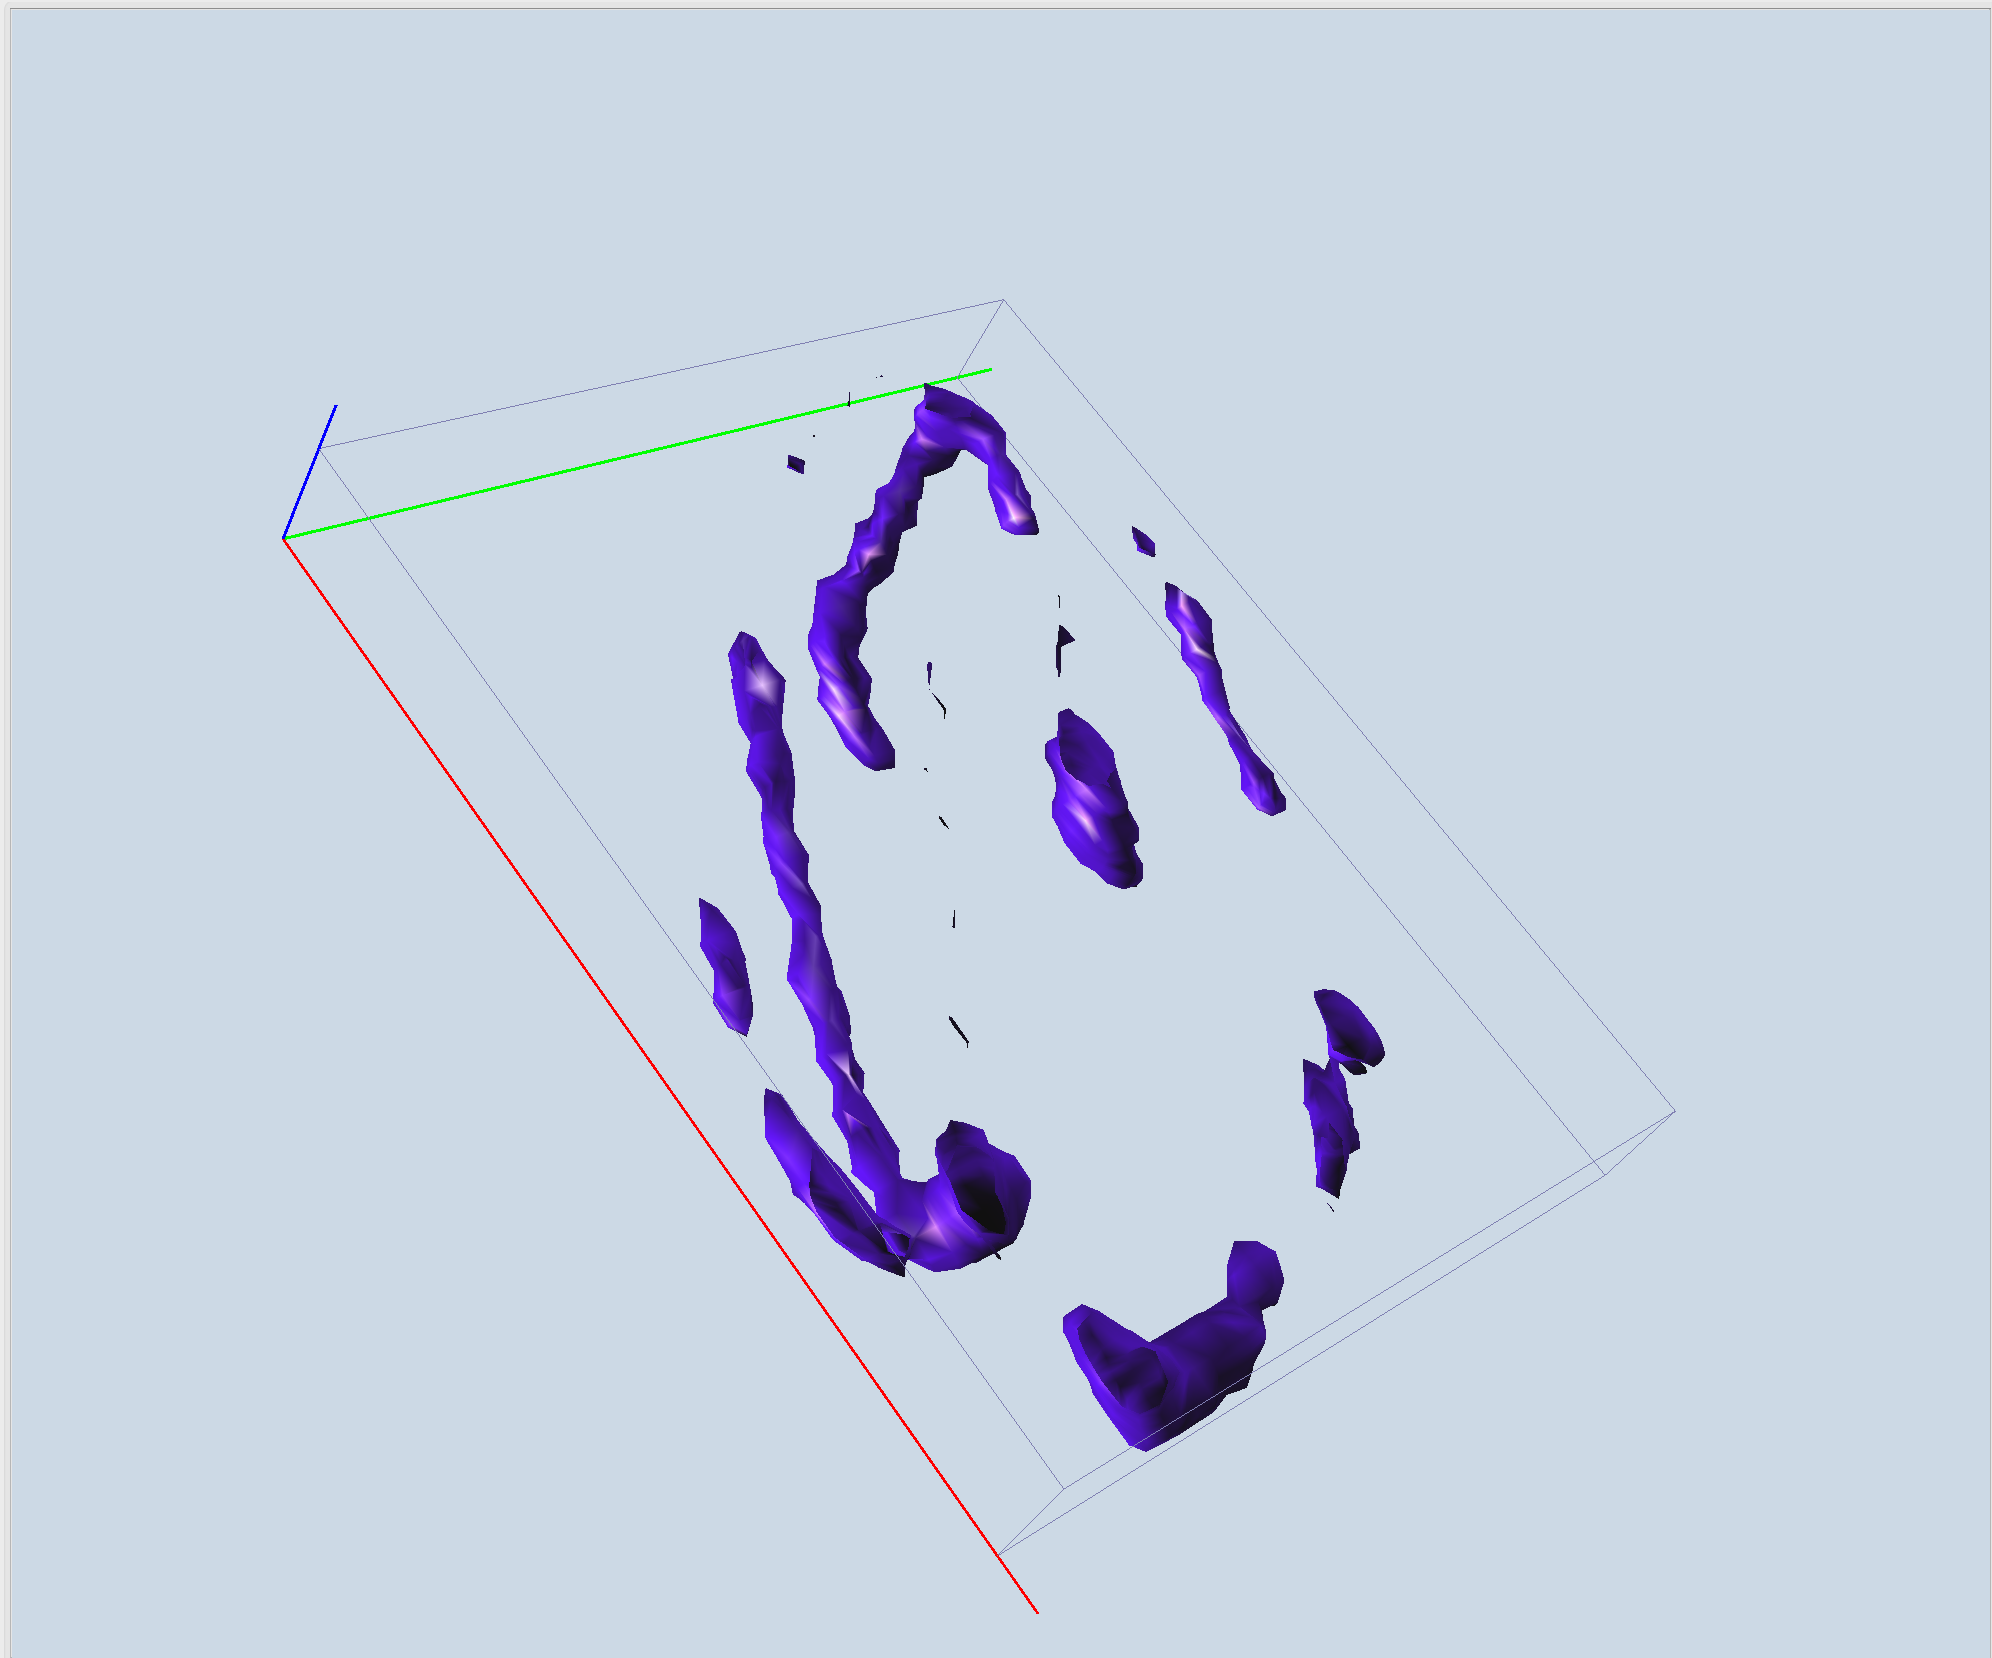
\includegraphics[width=0.3\linewidth]{Report/Images/6.3.2/150-255,50-sliced.png}
    \caption{Threshold: 150-255, mesh density:50, original (left), rotated (middle), cross-section(right)}
    \label{fig:surface_vis_150_255-50}
\end{figure}

\begin{figure}[h!]
    \centering
    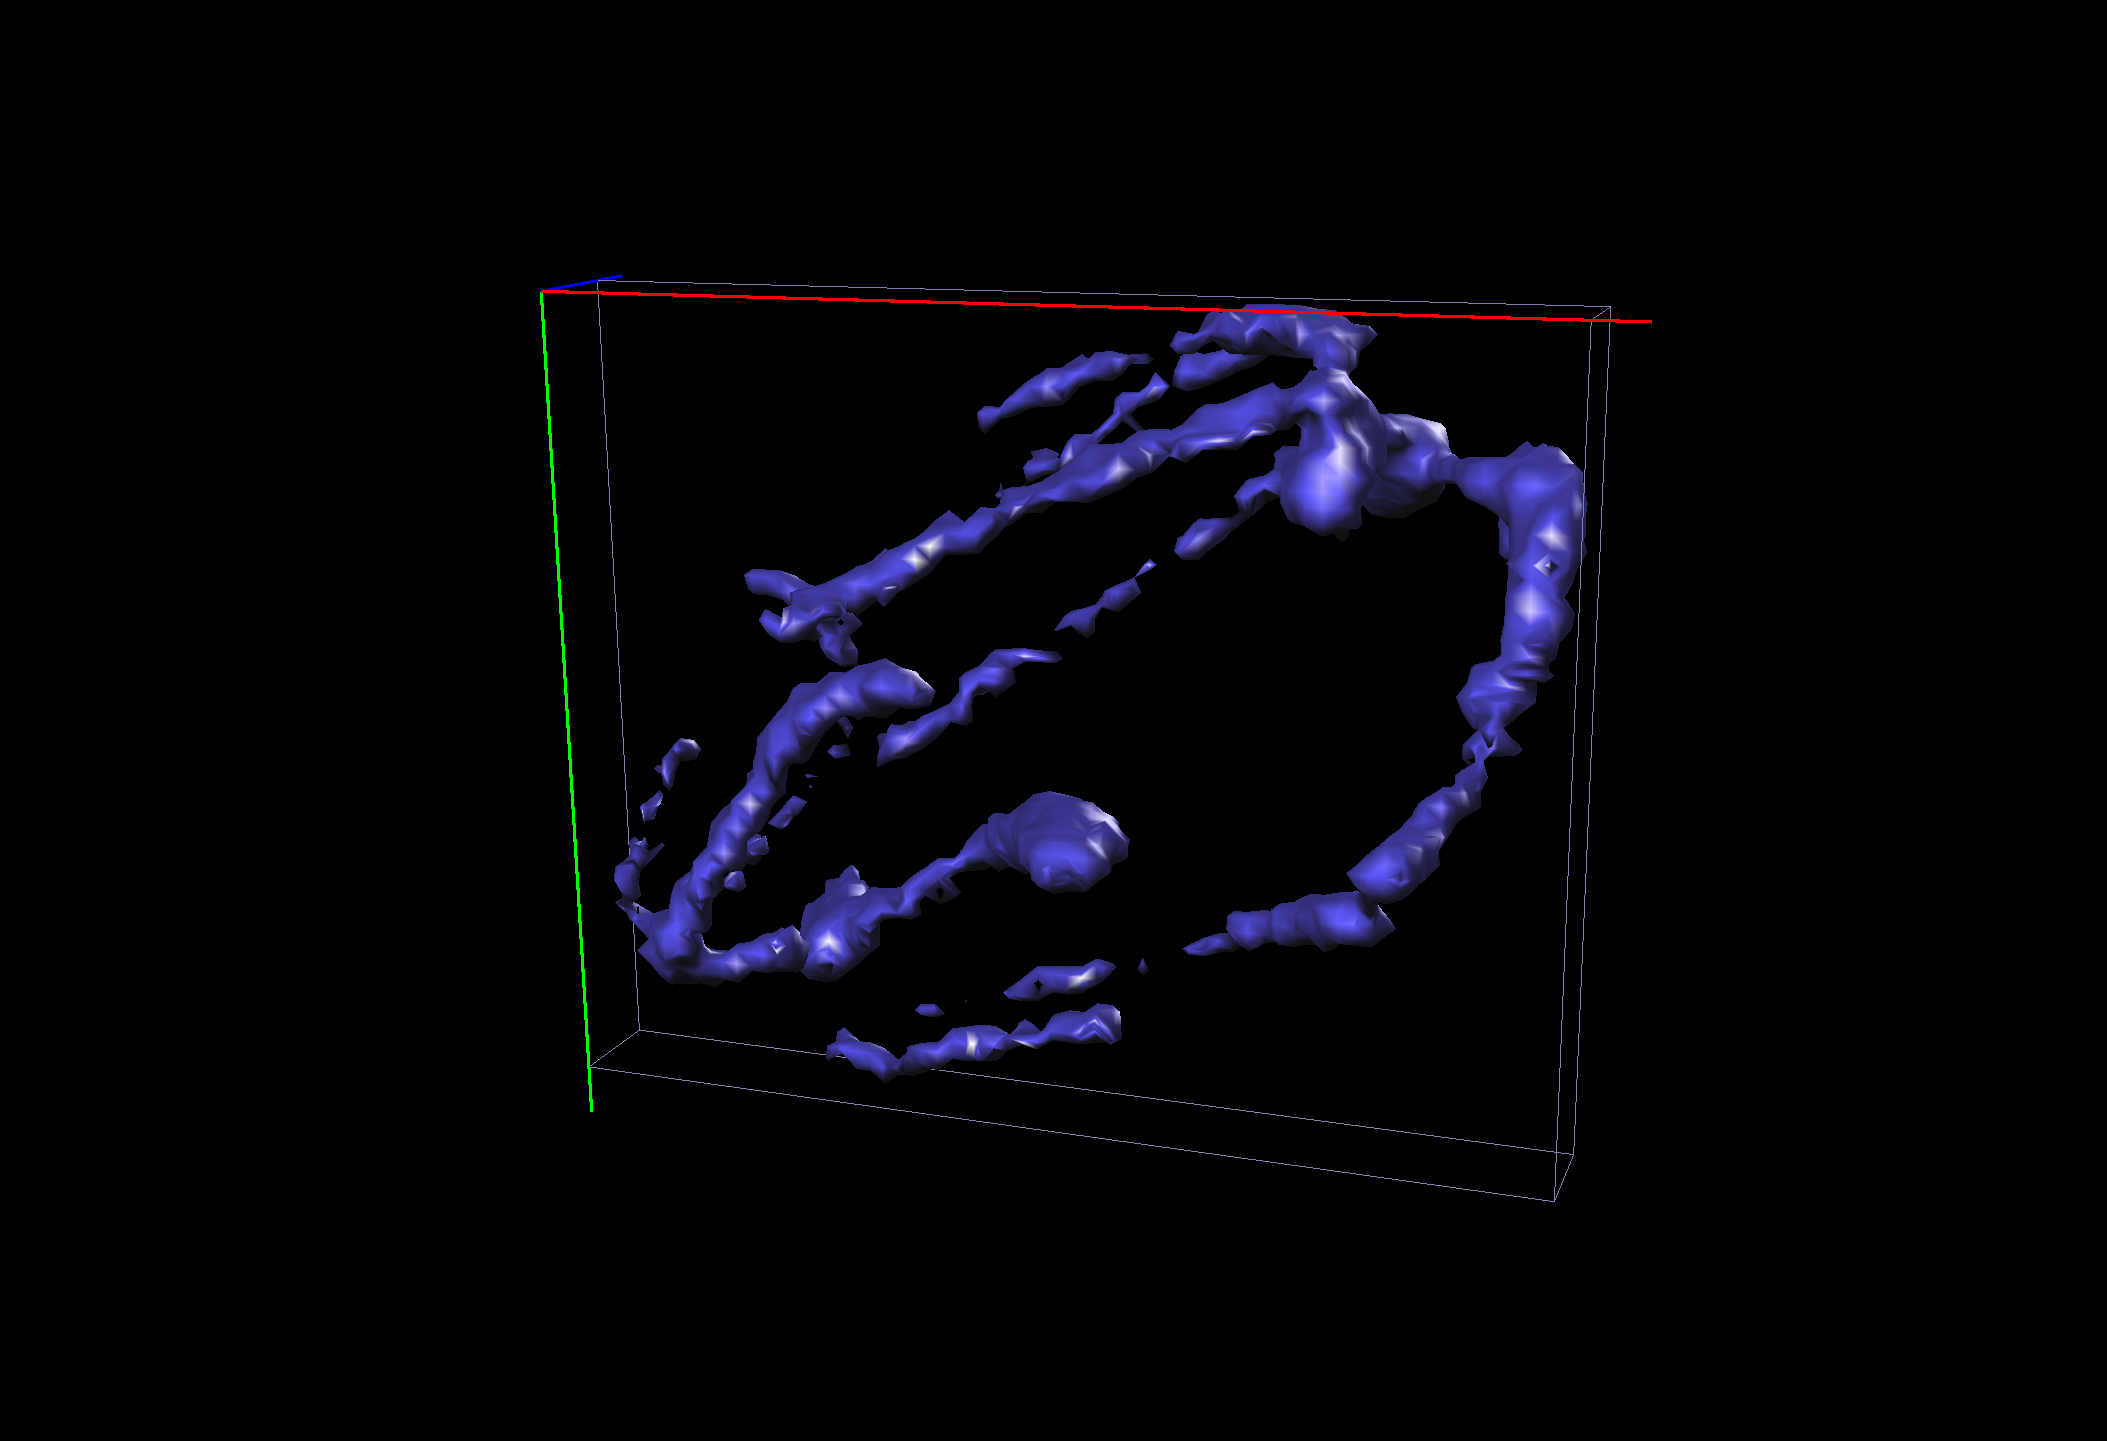
\includegraphics[width=0.3\linewidth]{Report/Images/6.3.2/150-255,75.png}
    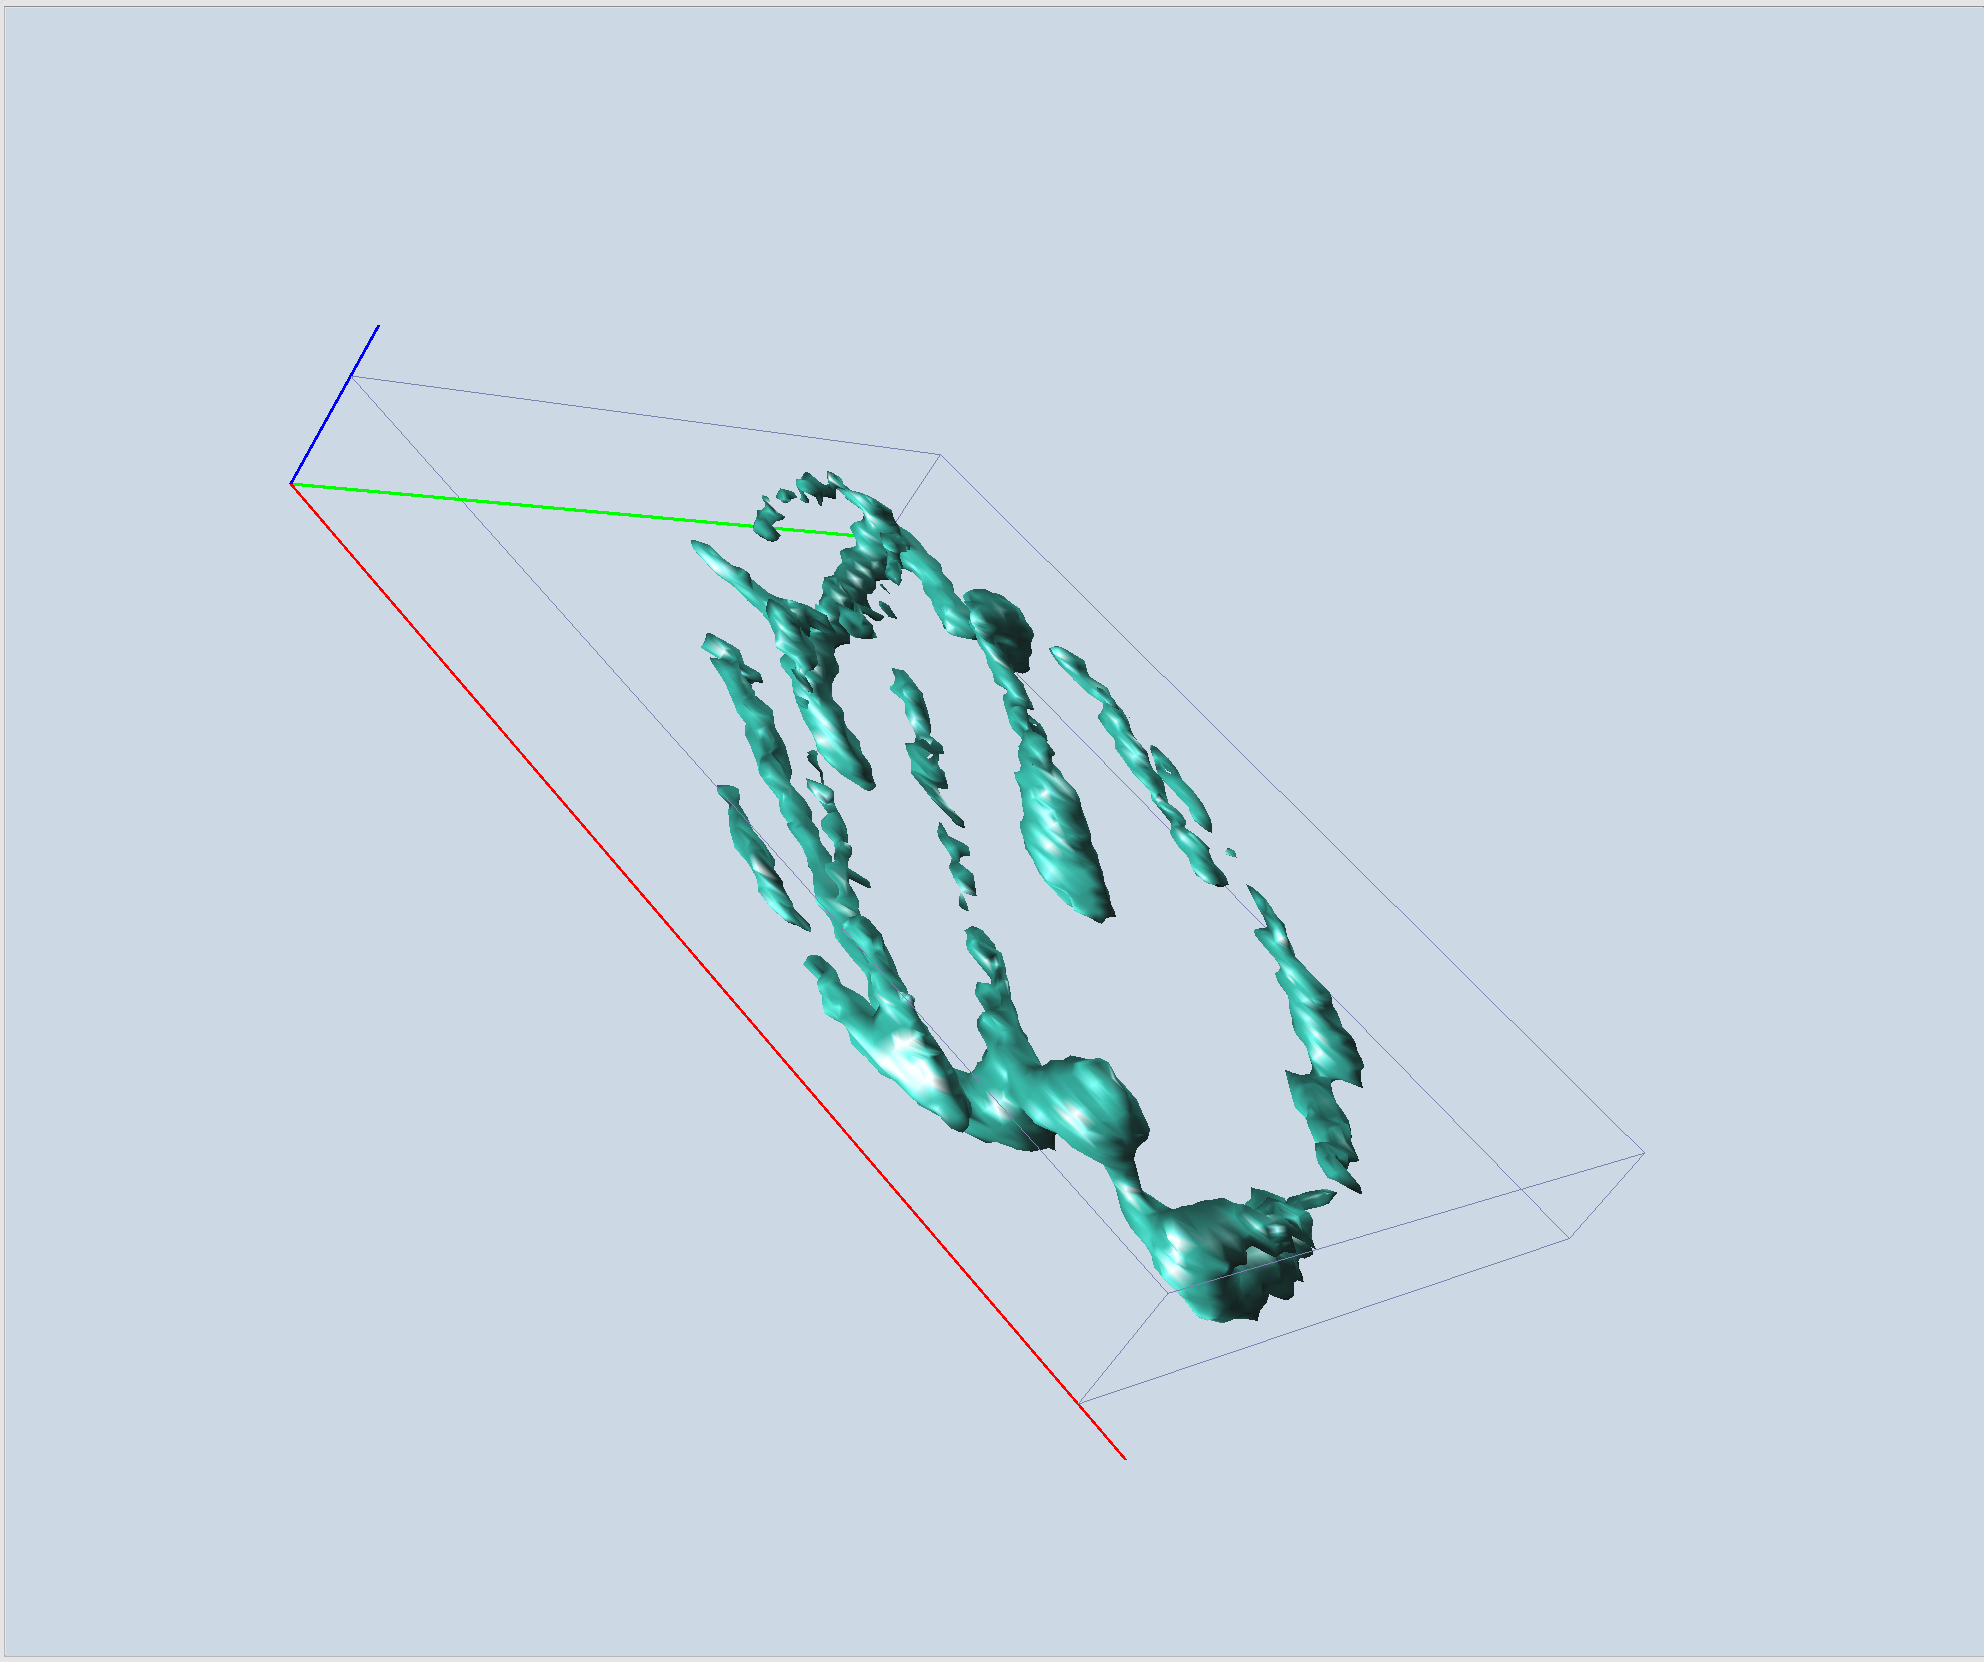
\includegraphics[width=0.3\linewidth]{Report/Images/6.3.2/150-255,75-rotated.png}
    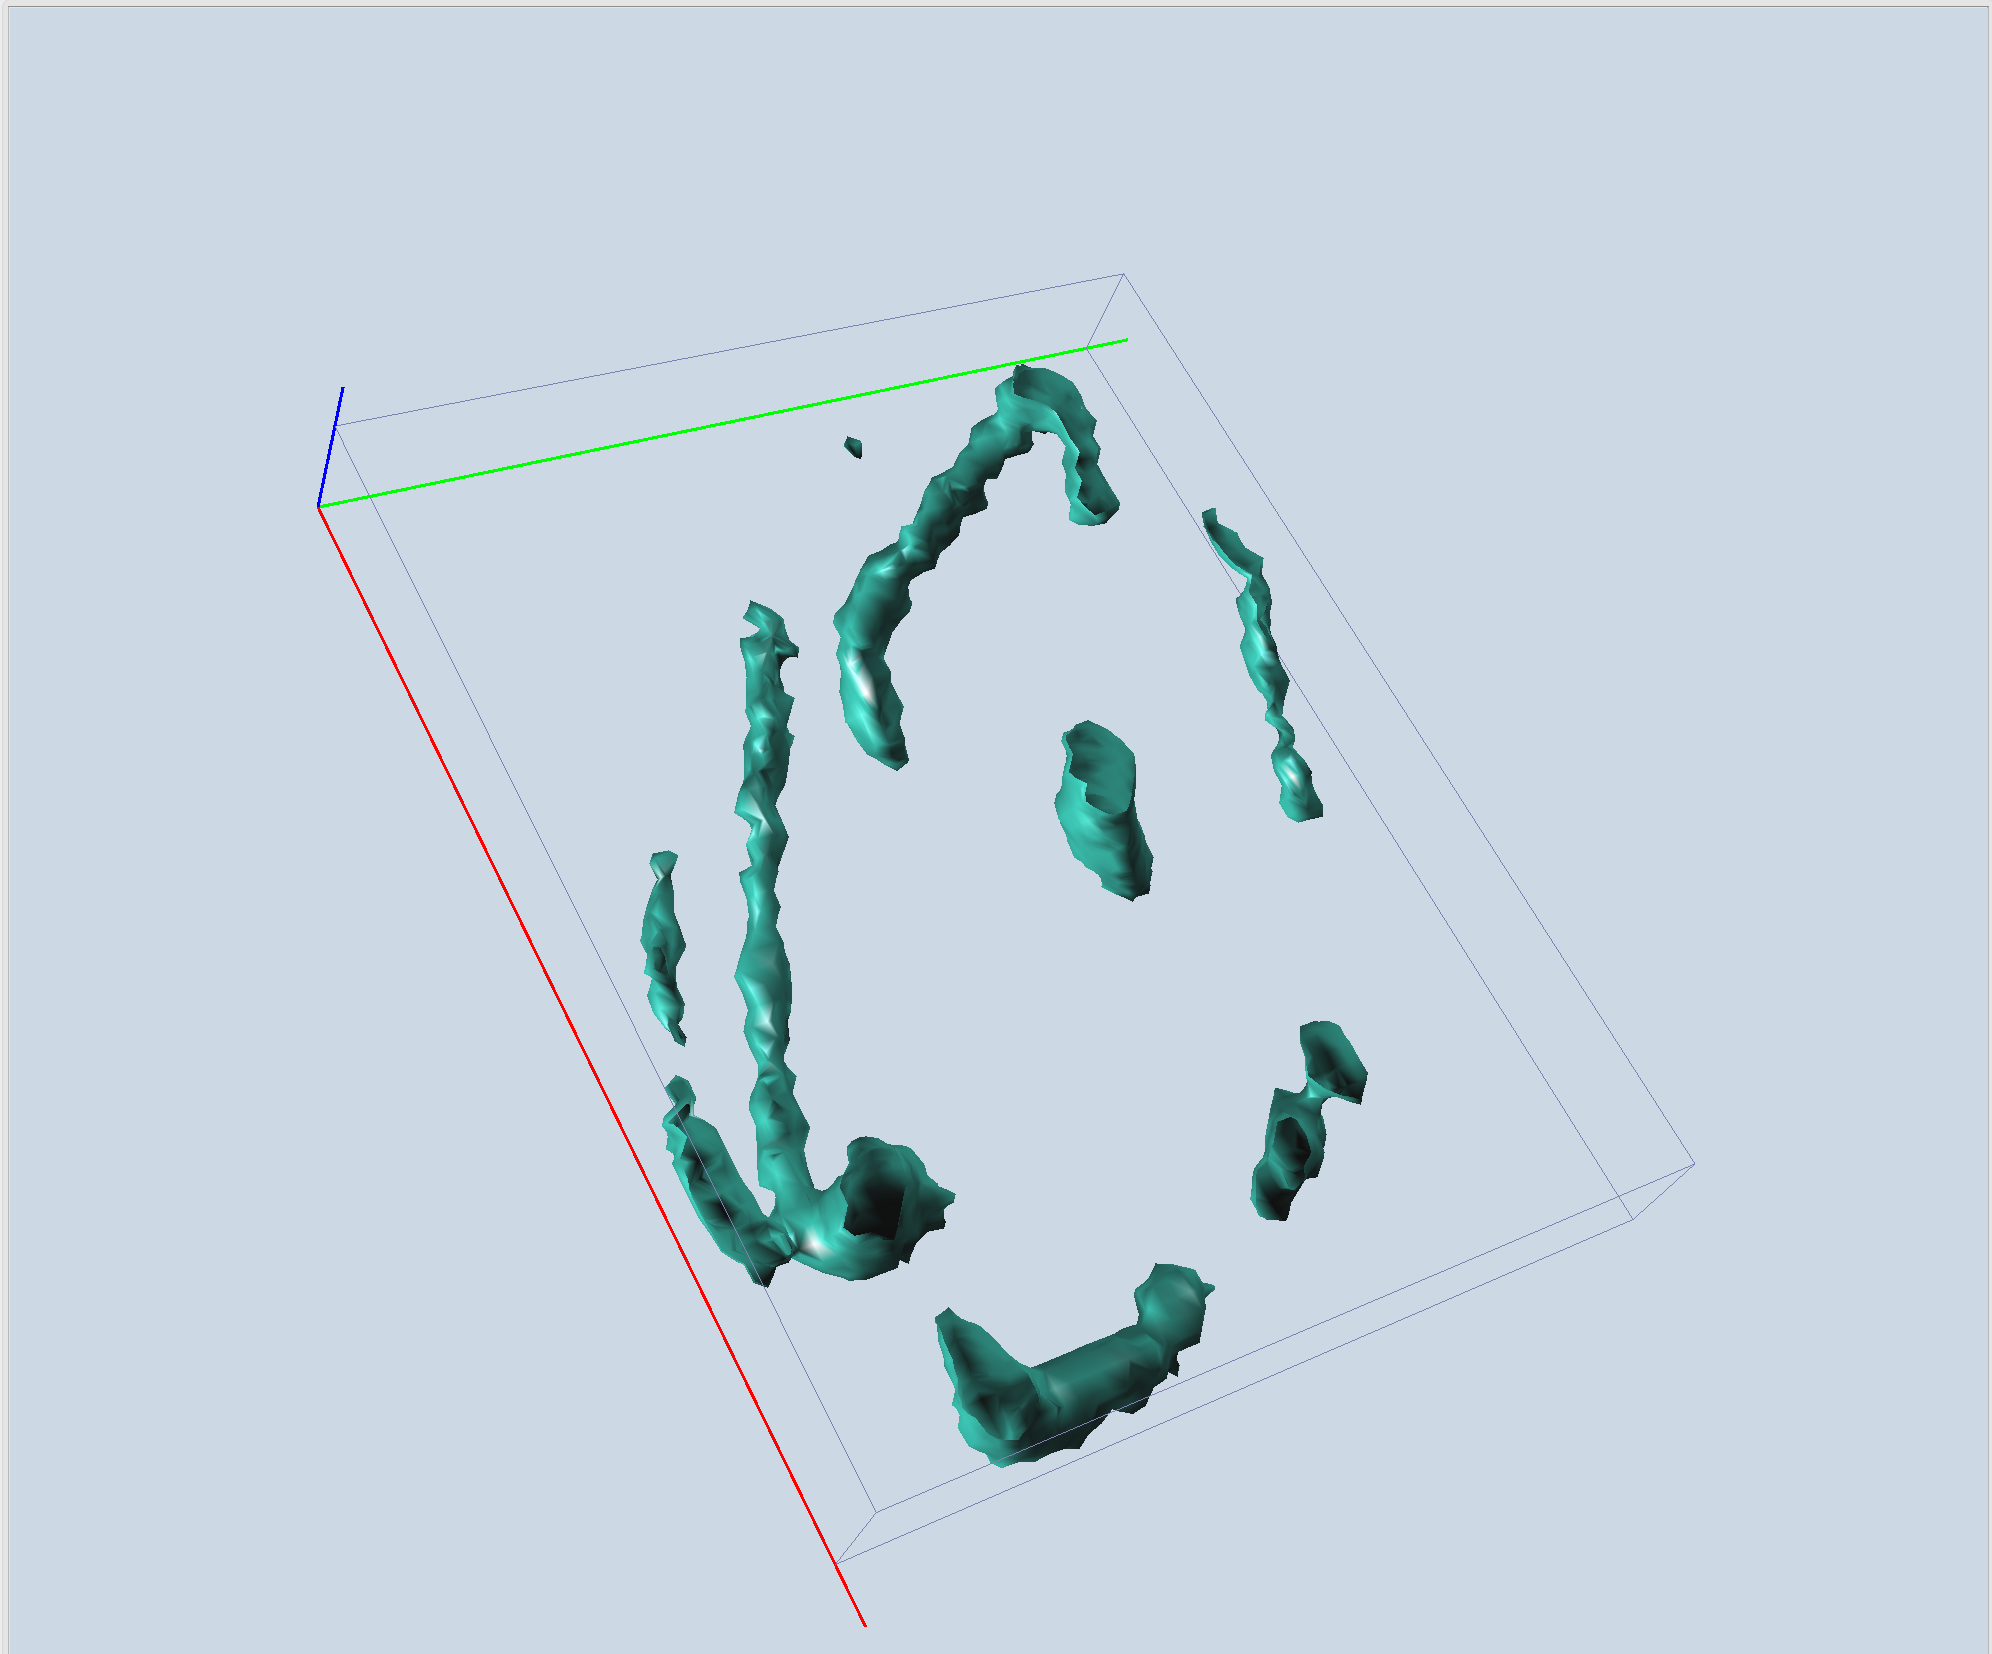
\includegraphics[width=0.3\linewidth]{Report/Images/6.3.2/150-255,75-sliced.png}
    \caption{Threshold: 150-255, mesh density:75, original (left), rotated (middle), cross-section(right)}
    \label{fig:surface_vis_150_255-75}
\end{figure}


\begin{figure}[h!]
    \centering
    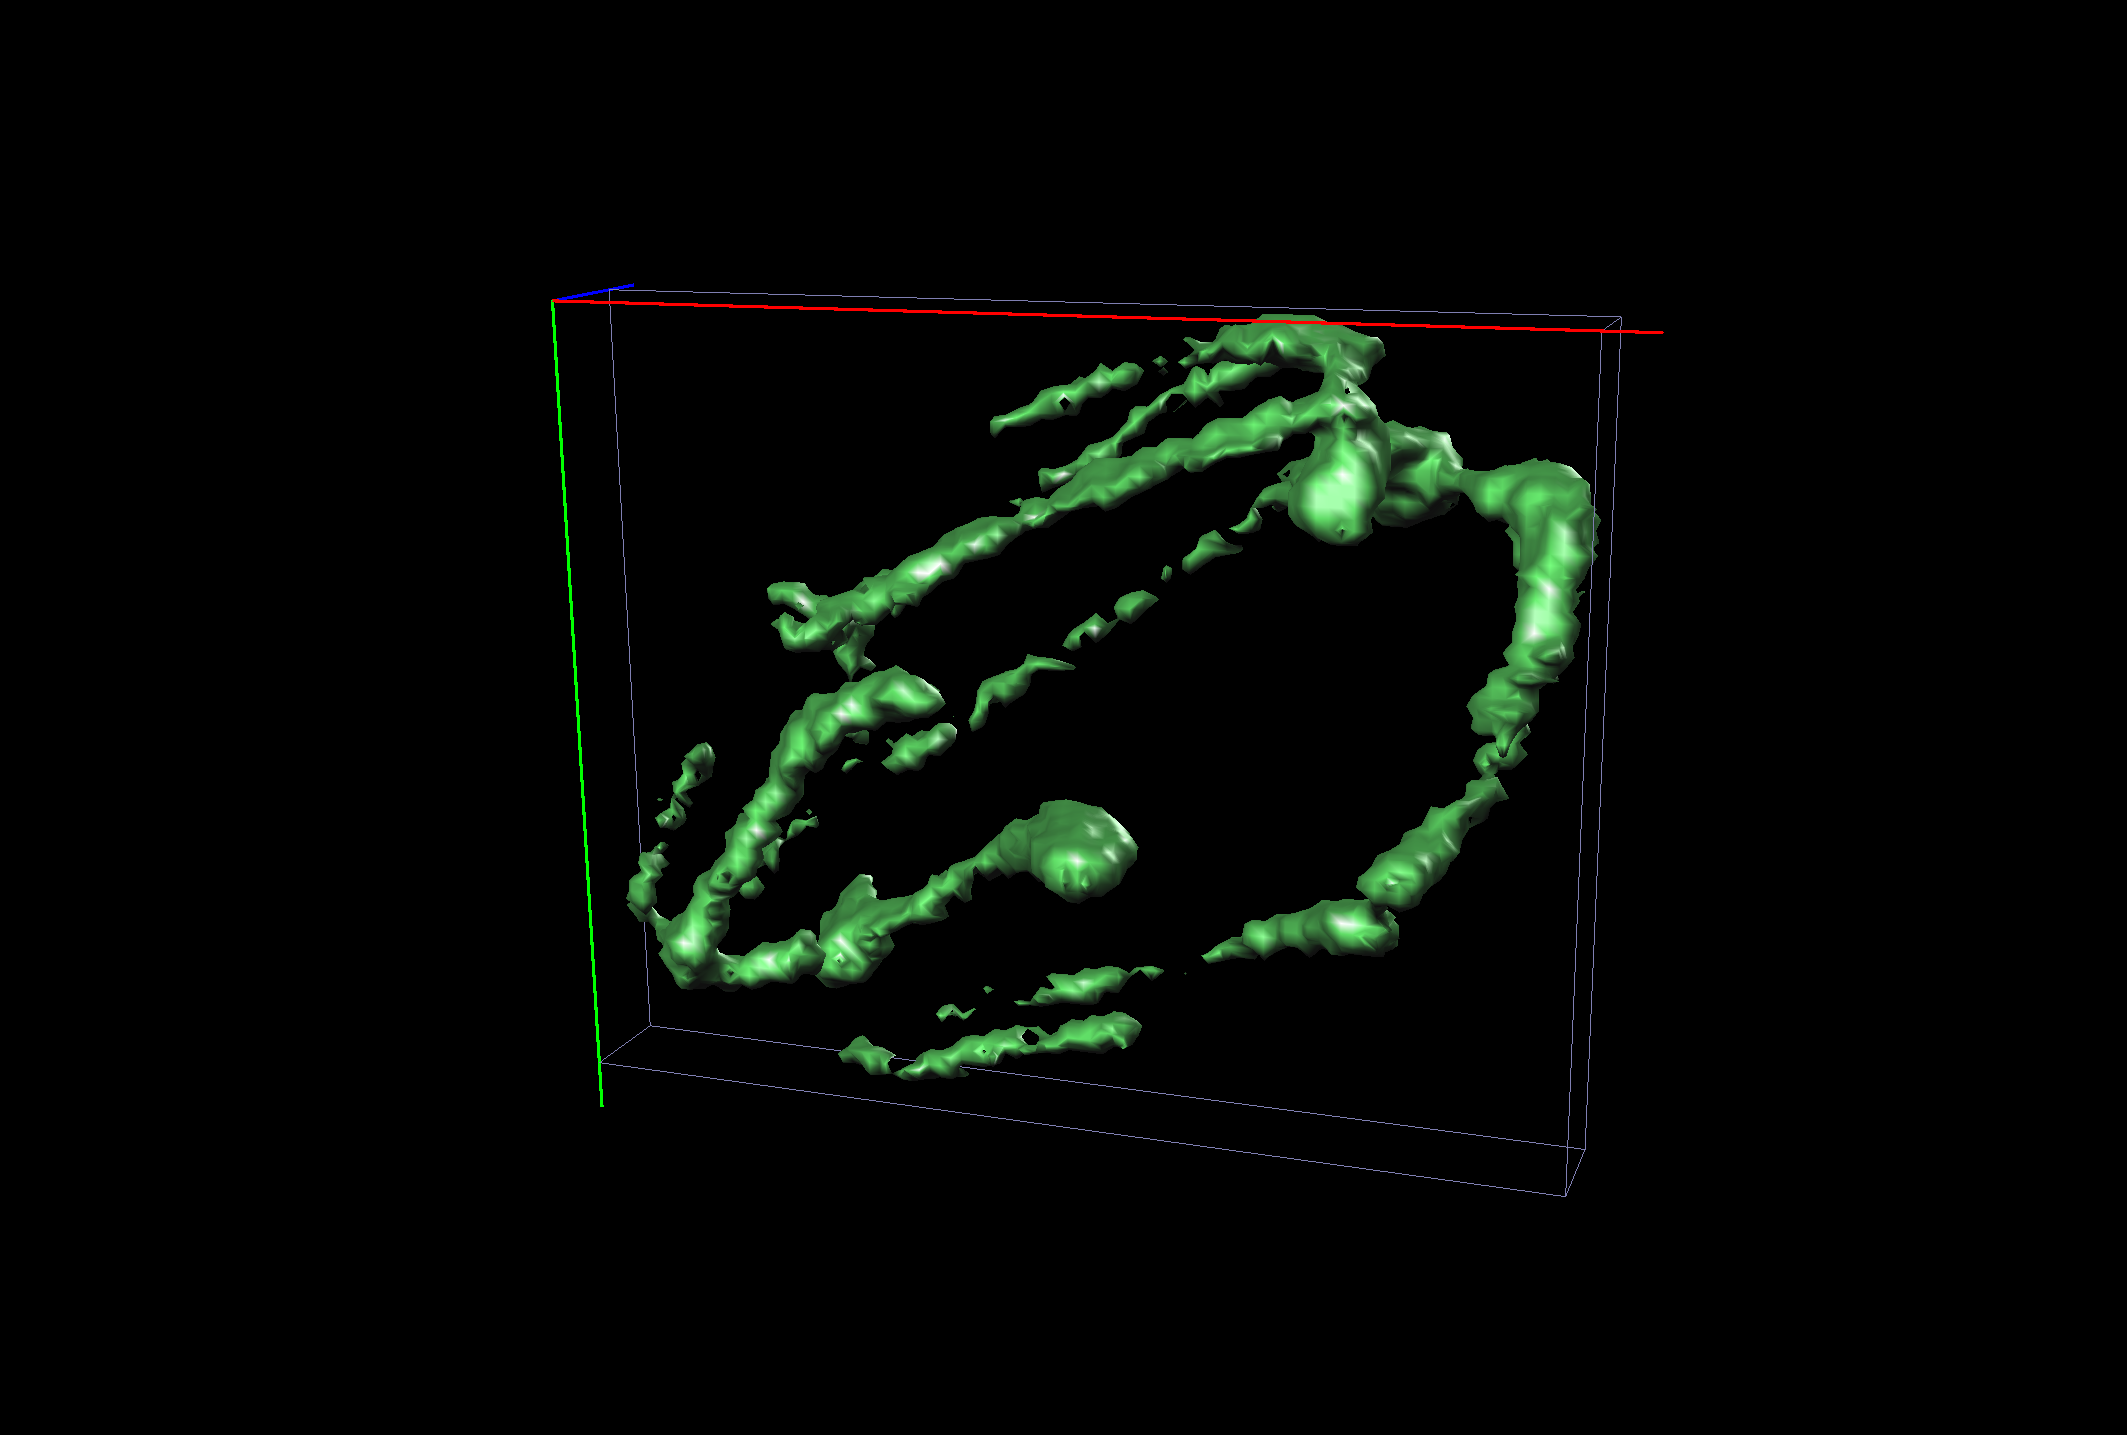
\includegraphics[width=0.3\linewidth]{Report/Images/6.3.2/150-255,100.png}
    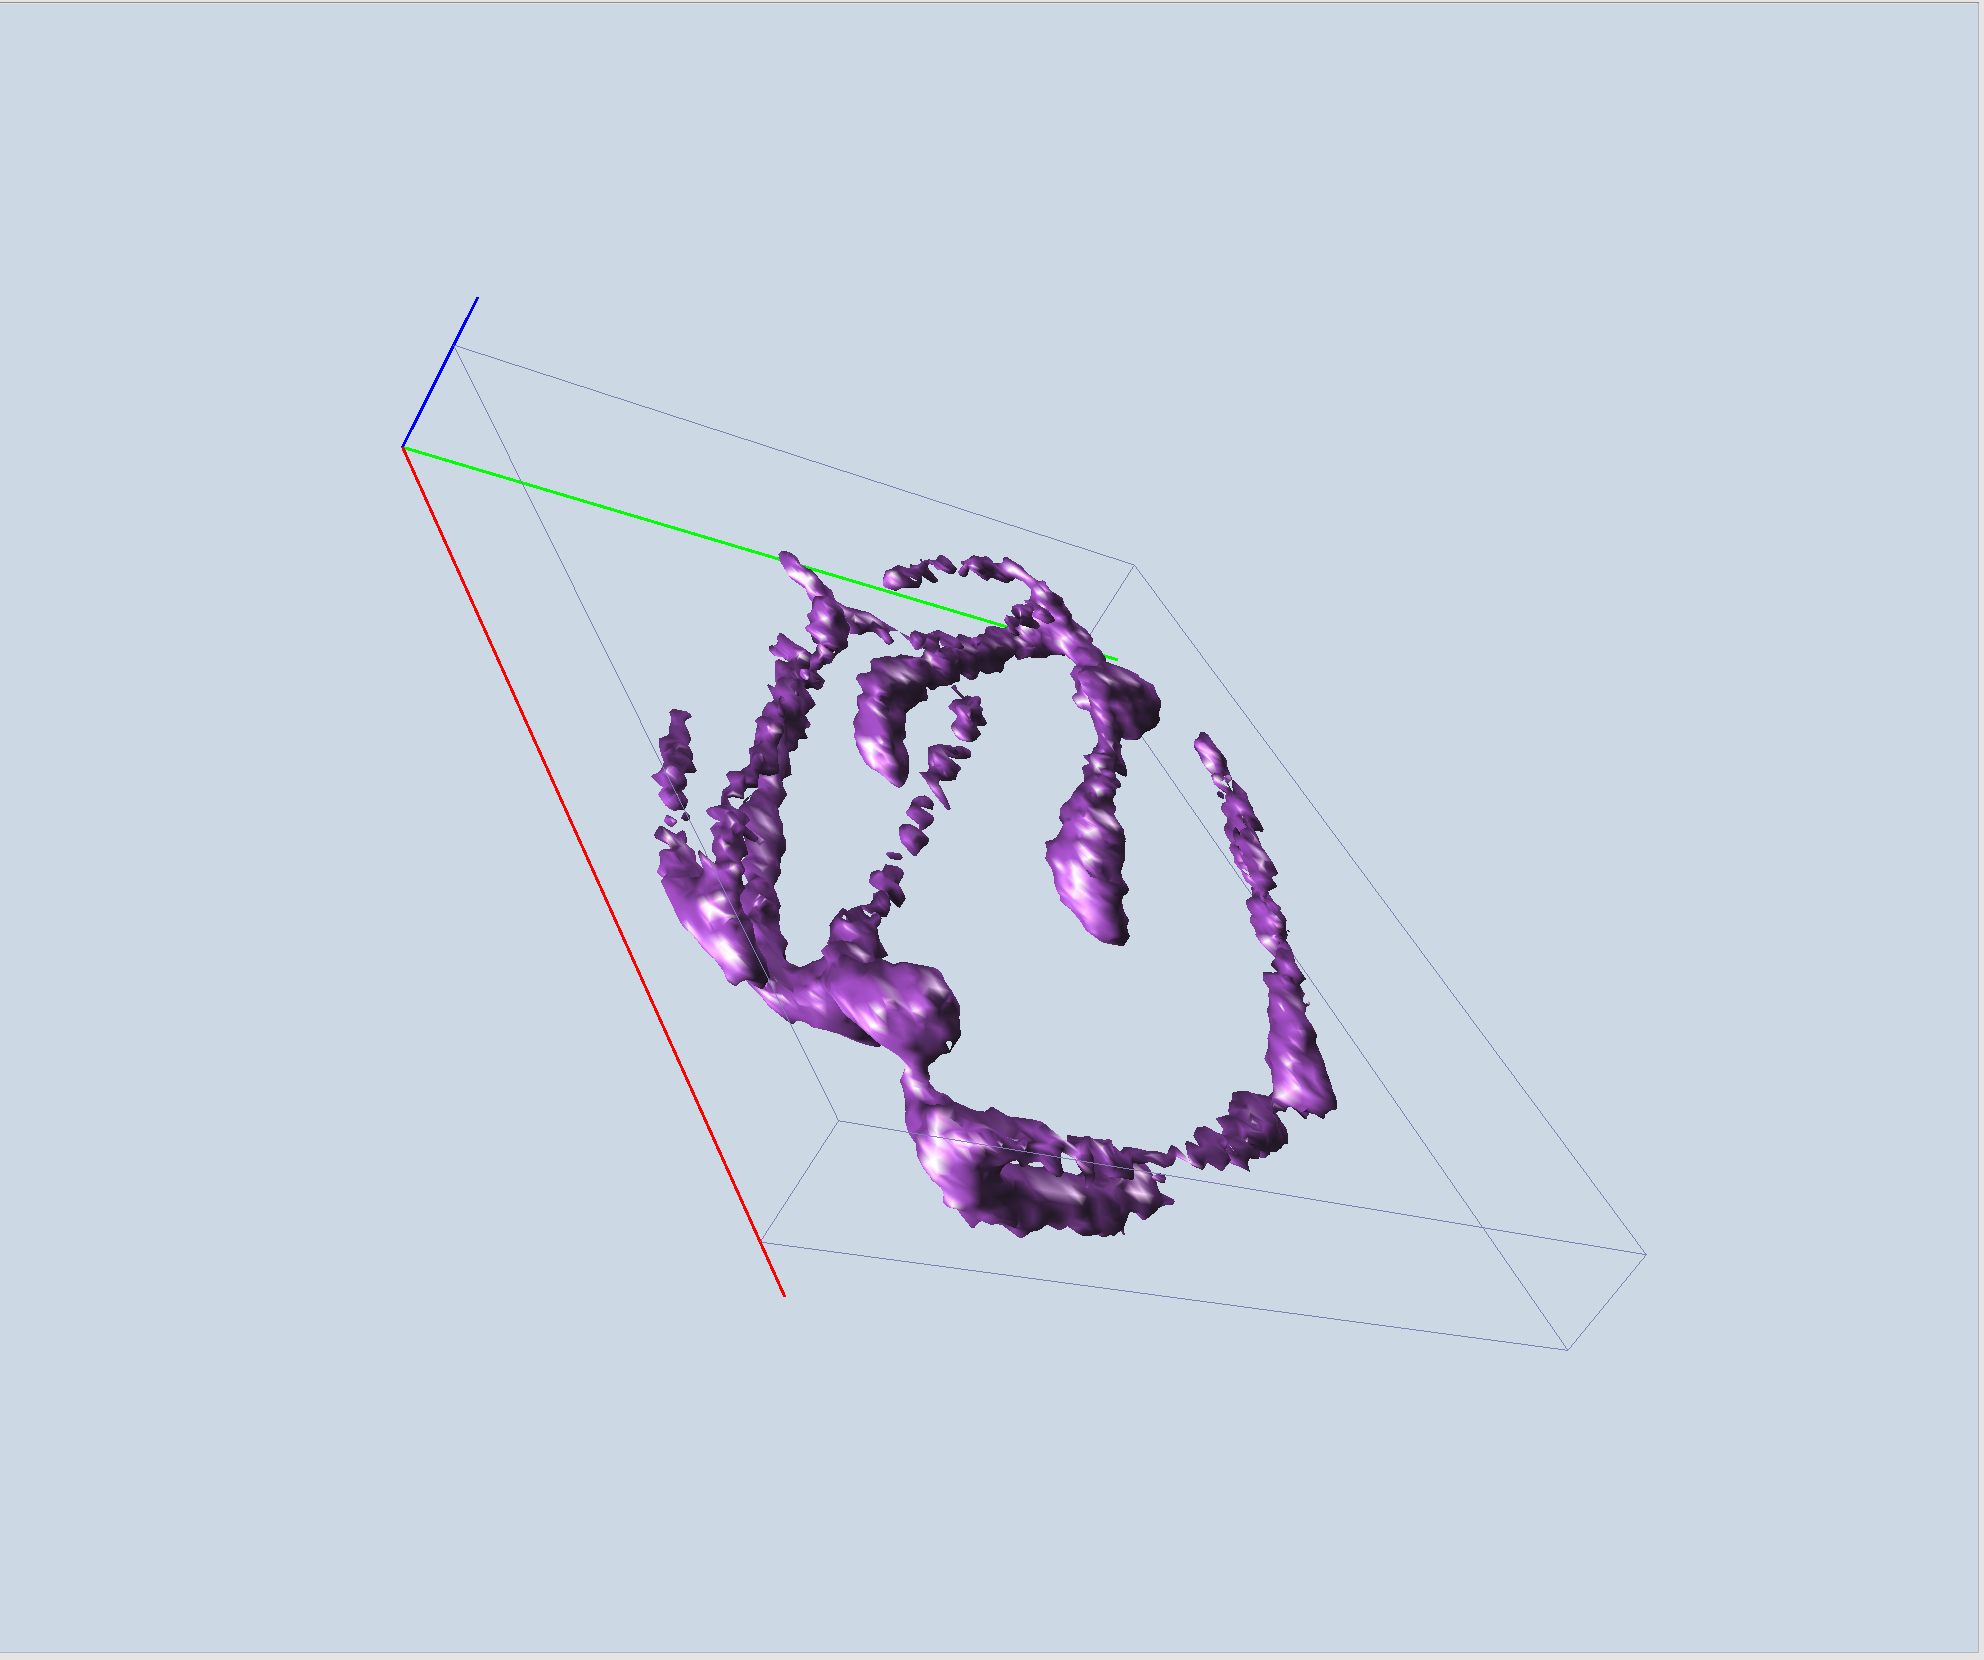
\includegraphics[width=0.3\linewidth]{Report/Images/6.3.2/150-255,100-rotated.png}
    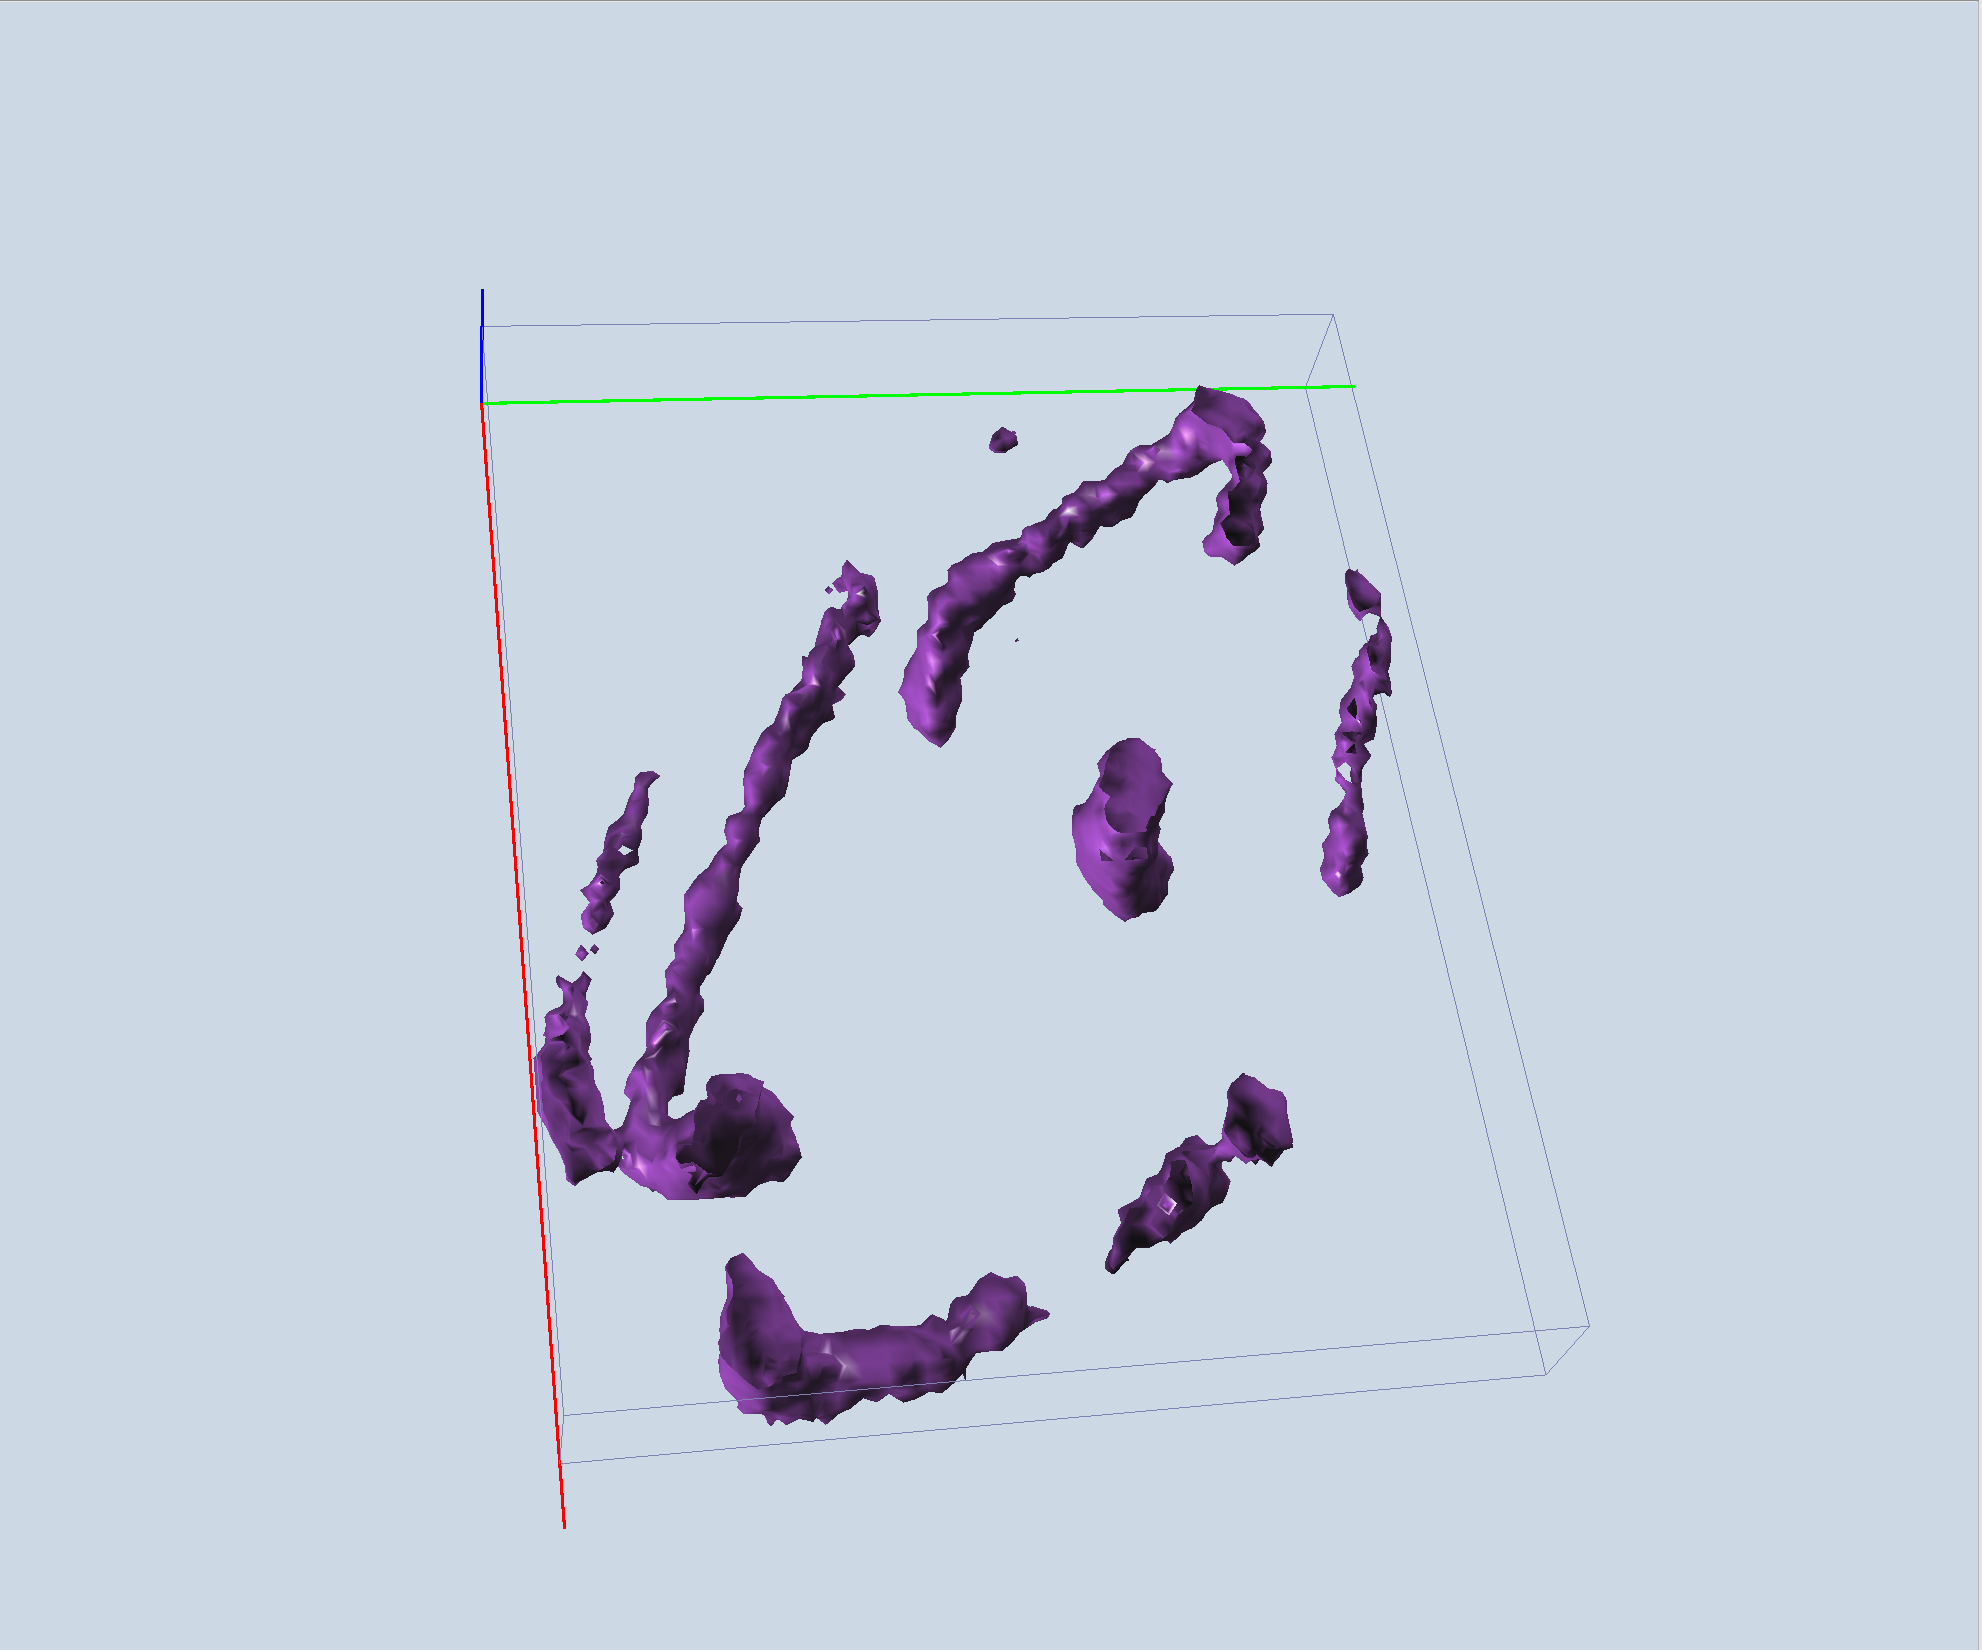
\includegraphics[width=0.3\linewidth]{Report/Images/6.3.2/150-255,100-sliced.png}
    \caption{Threshold: 75-150, mesh density:100, original (left), rotated (middle), cross-section(right)}
    \label{fig:surface_vis_150_255-100}
\end{figure}
\clearpage

\subsection*{Volume and Surface Visualization}
For this part, figures \ref{fig:median_otsu} and \ref{fig:mip} were used for surface and volume visualization.\\
Figure \ref{fig:depth-cue-volume-viz} shows the results of the volume visualization of the depth-cued image (\ref{fig:mip}). The threshold was set to 54, and the contrast was set to -23. This allowed to view the image properly, without any loss. Figure \ref{fig:depth-cue-surface-viz} shows the surface visualization for the same. \\
Figure \ref{fig:binary-image-volume-viz} shows the results of the binary image i.e., figure (\ref{fig:median_otsu}). The threshold was set to 45, and the contrast was set to +55. Since this is a binary image, the contrast was much higher. Figure \ref{fig:binary-image-surface-viz} shows the surface visualization for the same. \\


\begin{figure}[h!]
\centering
\subfloat{\label{fig:depth-cuing-volume_v1}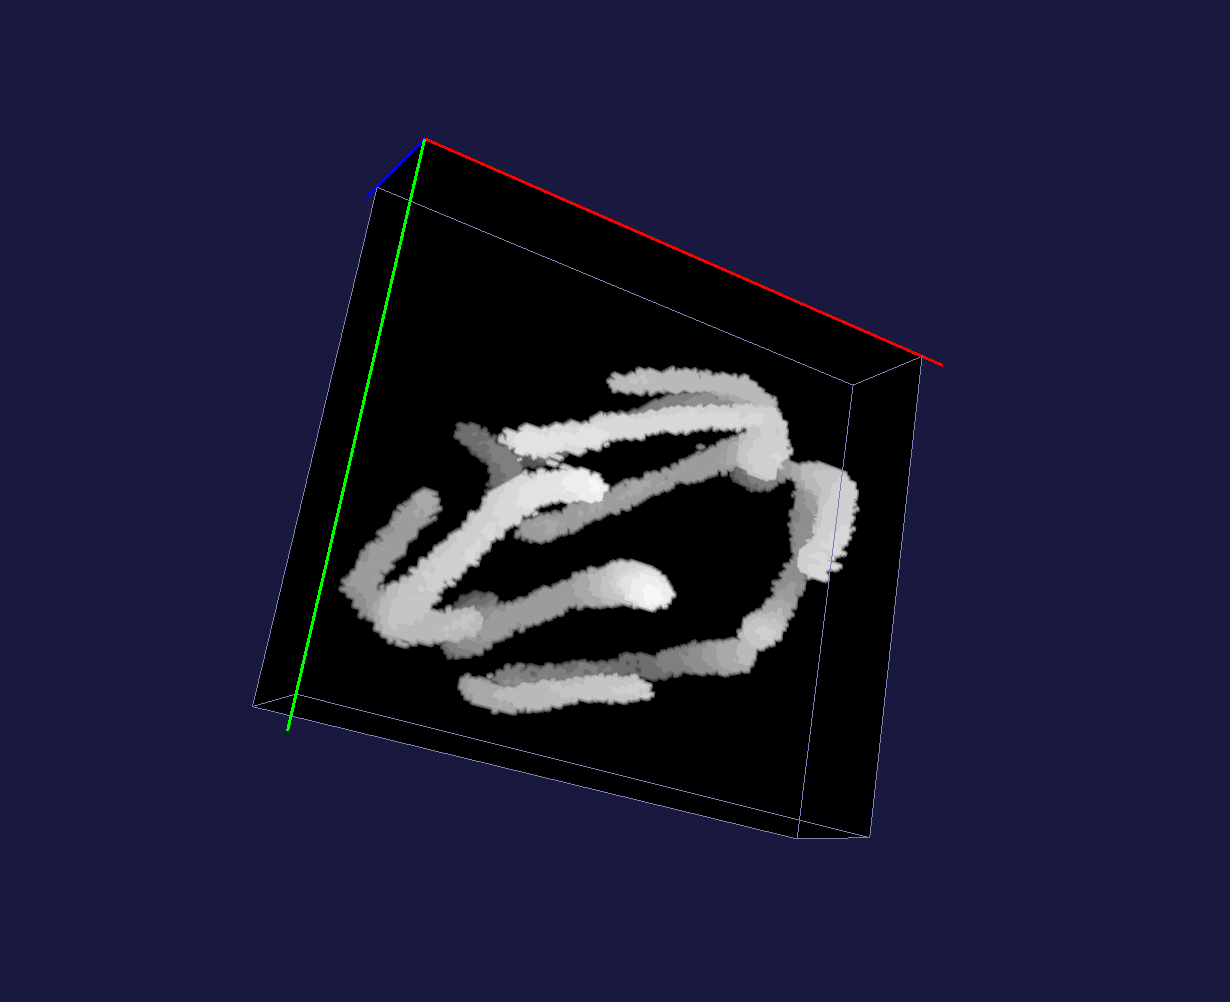
\includegraphics[width=0.45\textwidth]{Report/Images/6.3-7/Depth_Cuing_VolumeViz_t54_c-23_view1.png}}
\vspace{5 mm}
\subfloat{\label{fig:depth-cuing-volume_v2}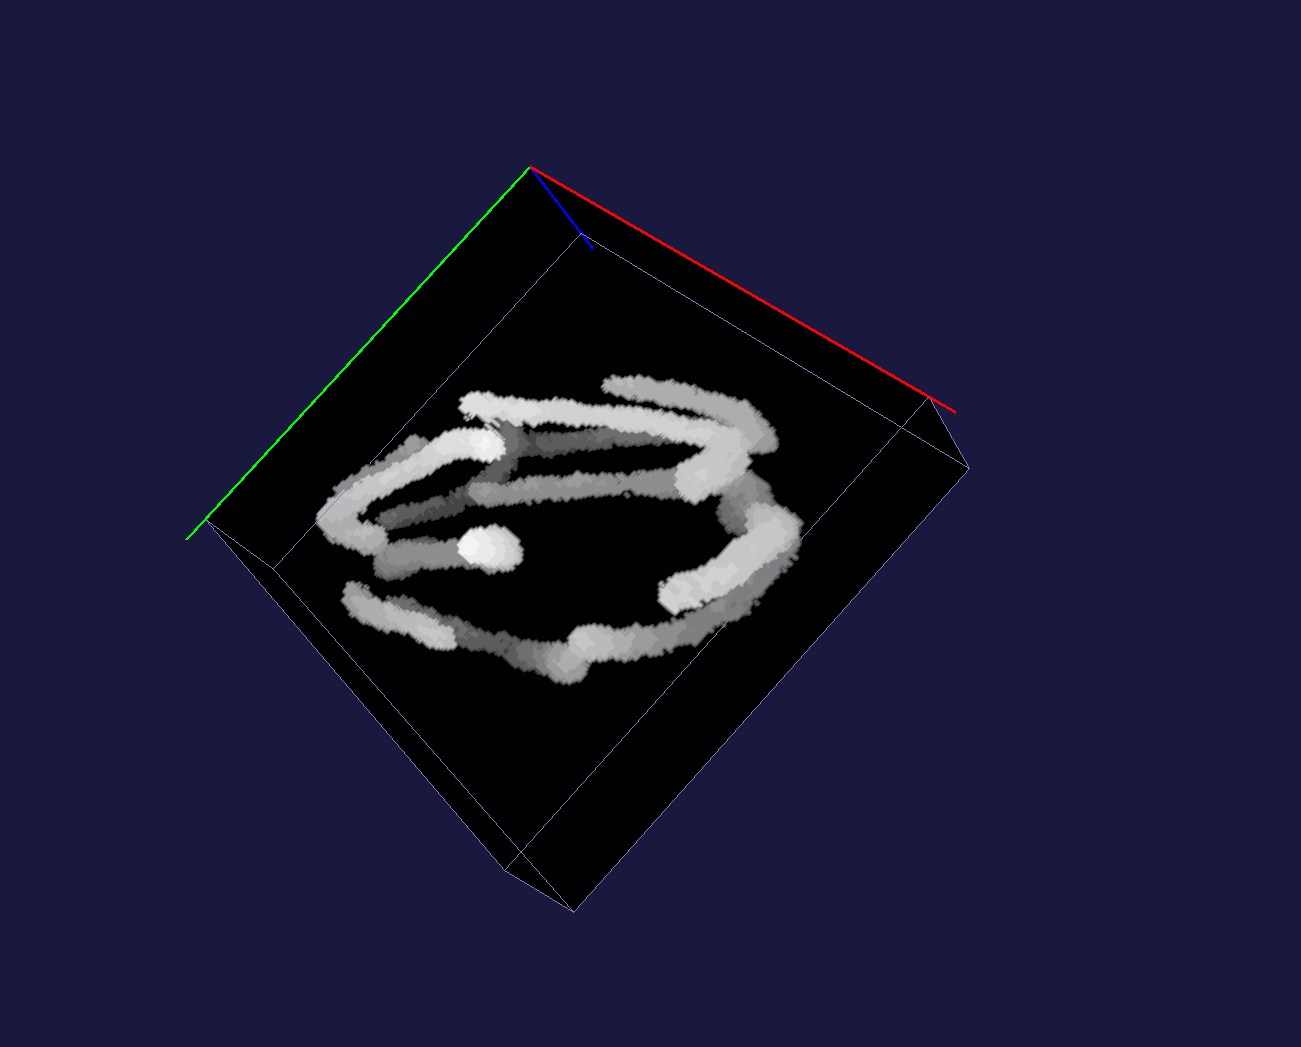
\includegraphics[width=0.45\textwidth]{Report/Images/6.3-7/Depth_Cuing_VolumeViz_t54_c-23_view2.png}}
\caption{Volume Visualization of the Depth-cued Image}
\label{fig:depth-cue-volume-viz}
\end{figure}
\begin{figure}[h!]
\centering
\subfloat{\label{fig:depth-cuing-surface_v1}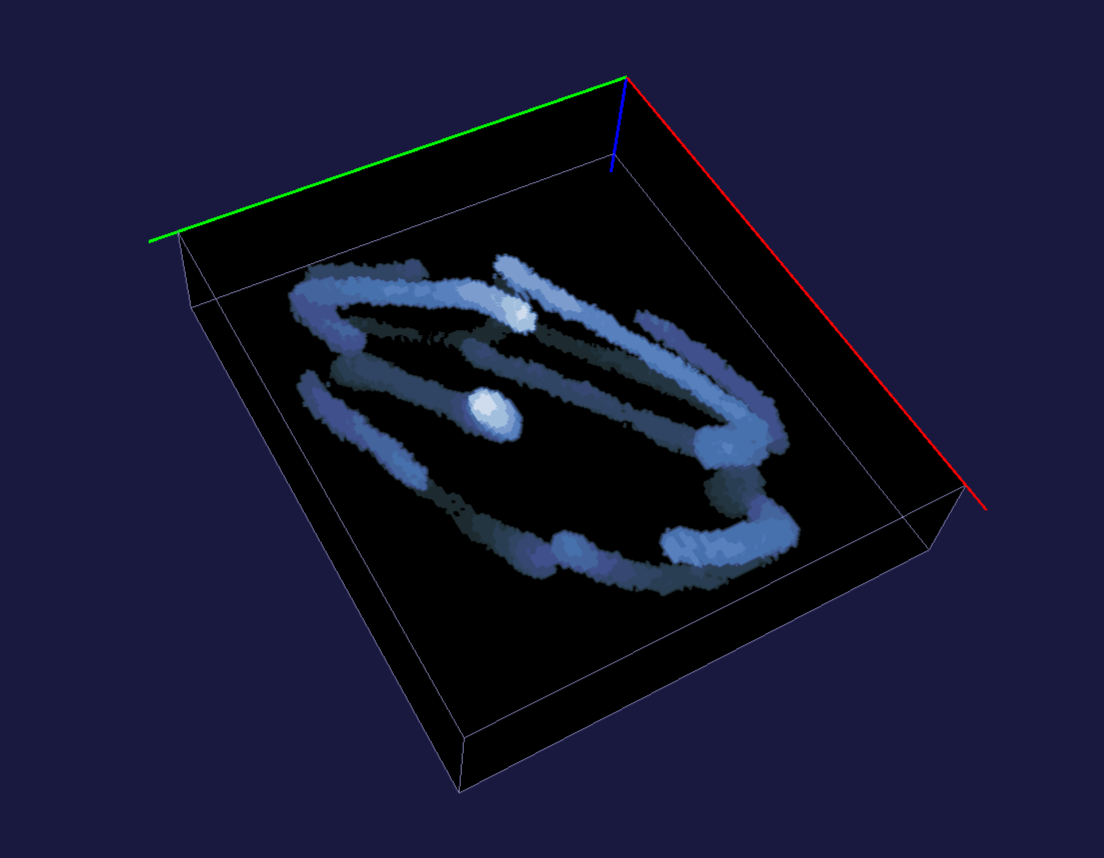
\includegraphics[width=0.45\textwidth]{Report/Images/6.3-7/DepthCuing_SurfaceVisualization_view1.png}}
\vspace{5 mm}
\subfloat{\label{fig:depth-cuing-surface_v2}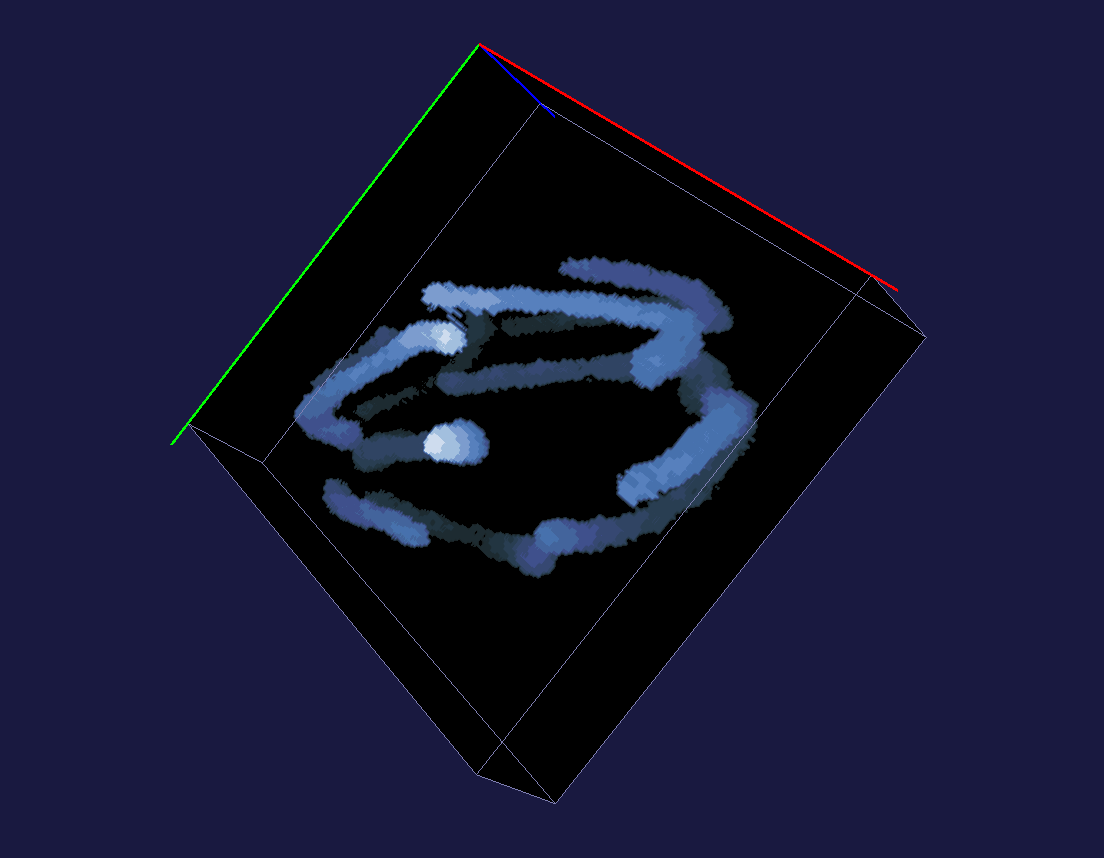
\includegraphics[width=0.45\textwidth]{Report/Images/6.3-7/DepthCuing_SurfaceVisualization_view2.png}}
\caption{Surface Visualization of the Depth-cued Image}
\label{fig:depth-cue-surface-viz}
\end{figure}

\begin{figure}[h!]
\centering
\subfloat{\label{fig:median-otsu-volume_v1}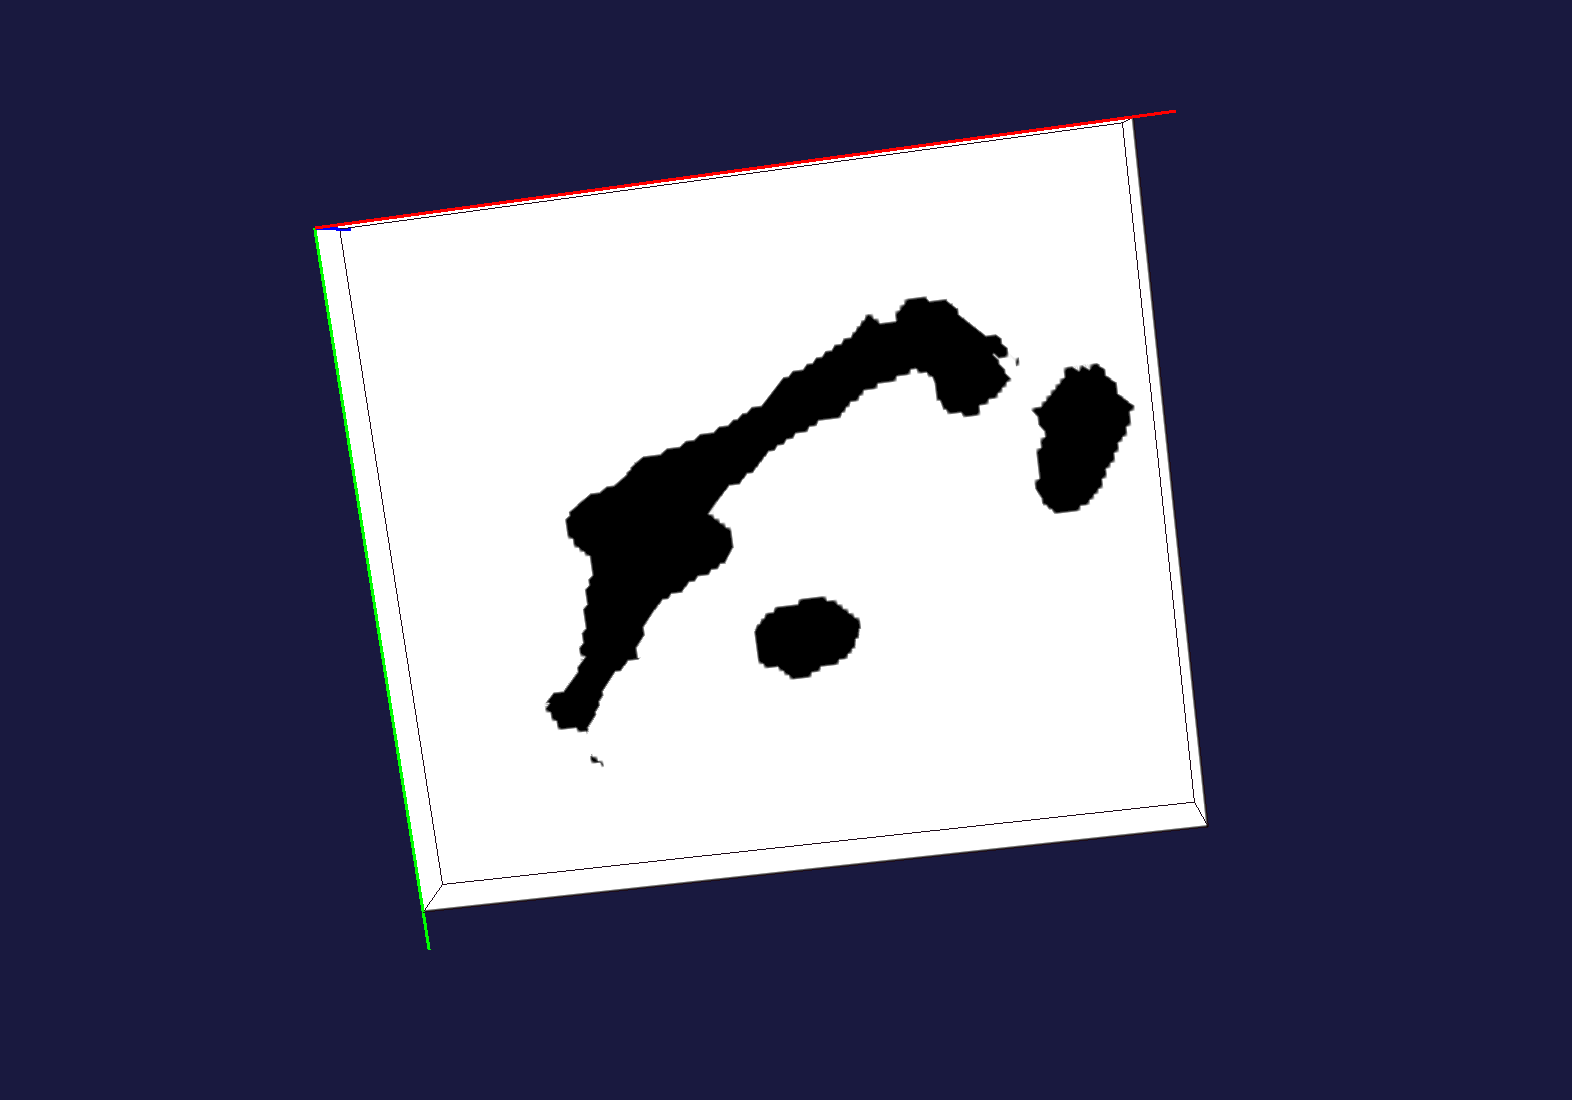
\includegraphics[width=0.45\textwidth]{Report/Images/6.3-7/BinaryImage_VolumeVisualization_t43_c55_view1.png}}
\vspace{5 mm}
\subfloat{\label{fig:median-otsu-volume_v2}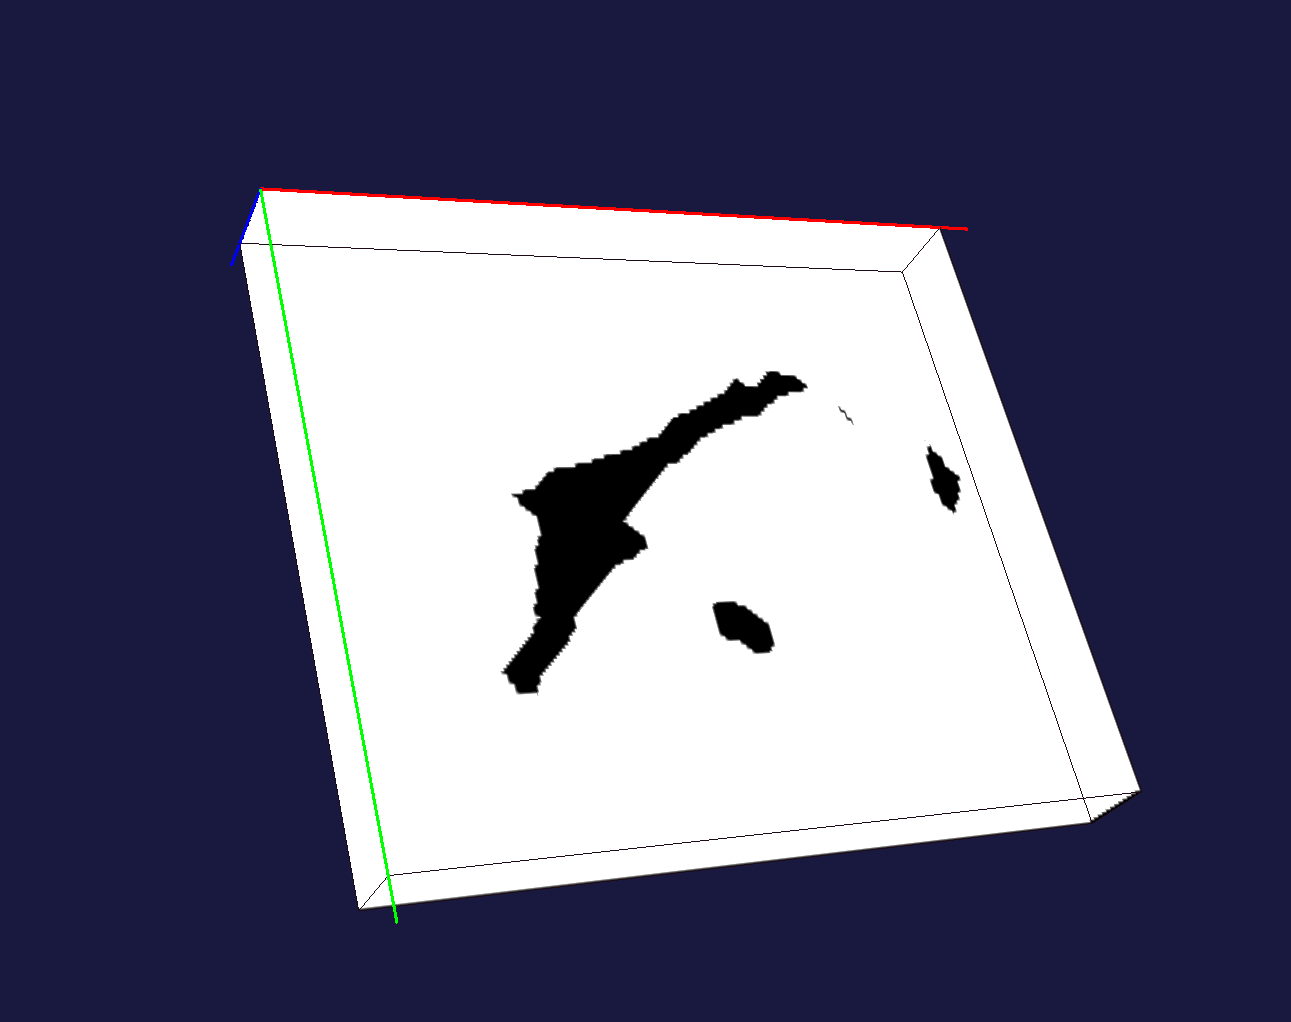
\includegraphics[width=0.45\textwidth]{Report/Images/6.3-7/BinaryImage_VolumeVisualization_t43_c55_view2.png}}
\caption{Volume Visualization of the Binary Image}
\label{fig:binary-image-volume-viz}
\end{figure}

\begin{figure}[h!]
\centering
\subfloat{\label{fig:median-otsu-surface_v1}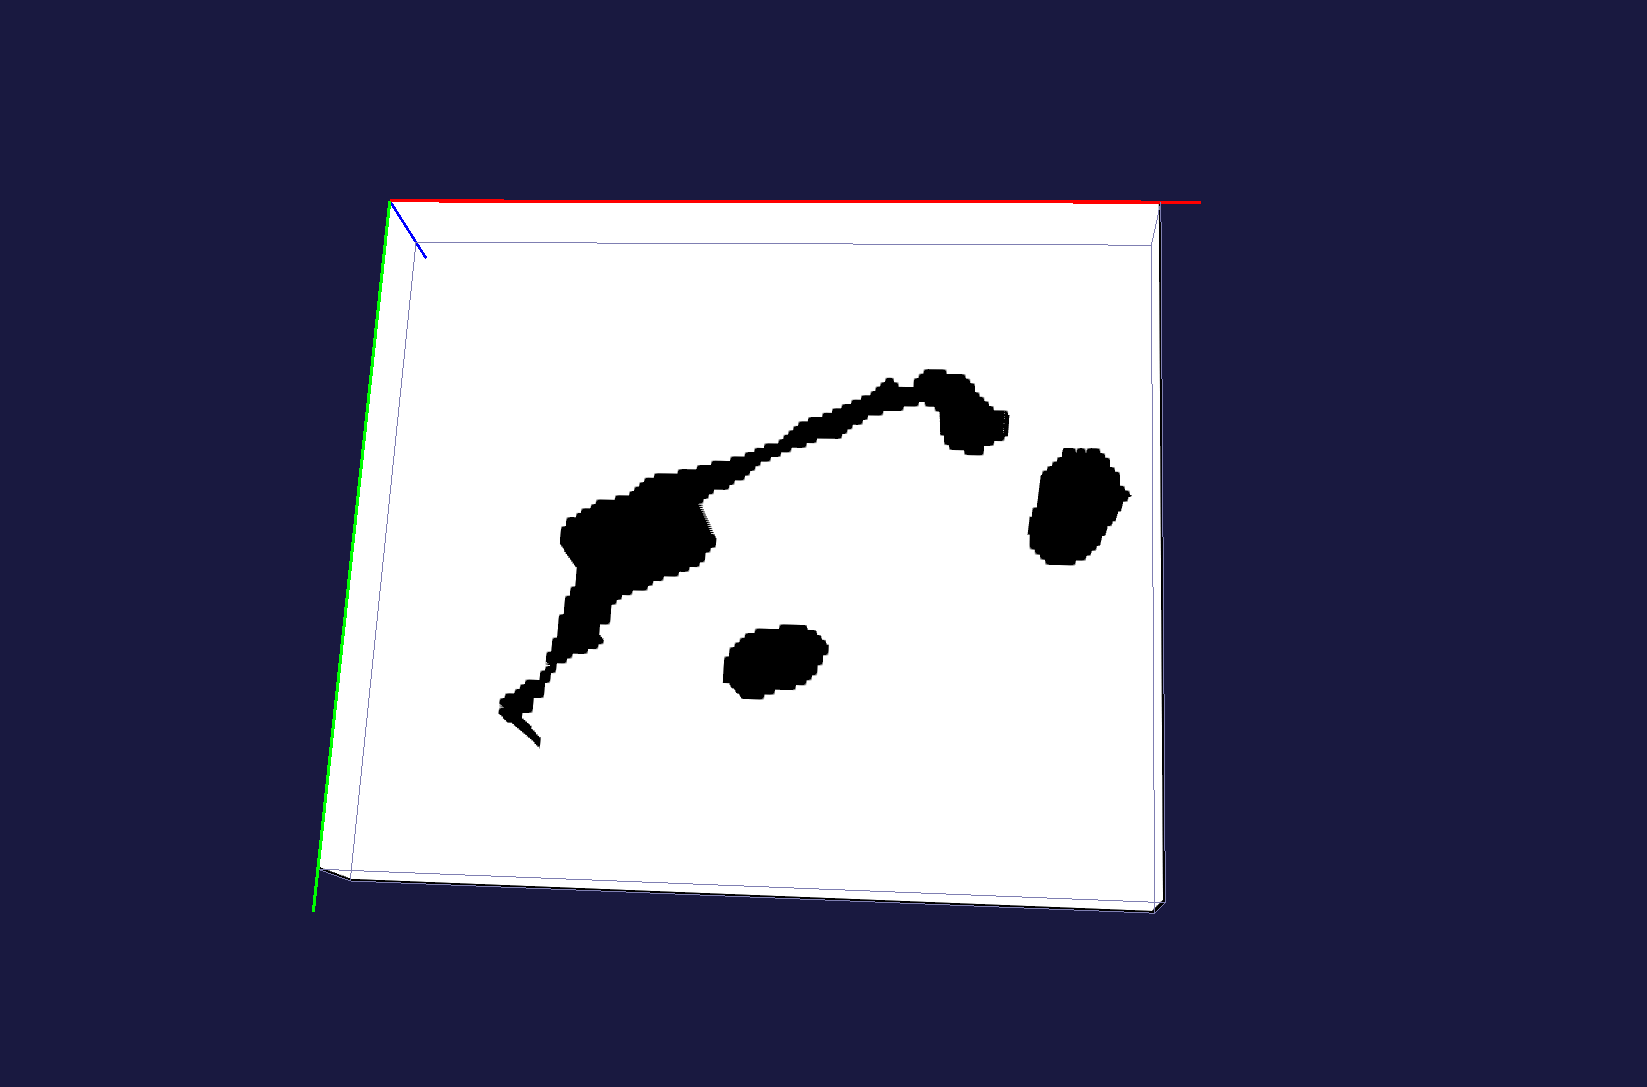
\includegraphics[width=0.45\textwidth]{Report/Images/6.3-7/BinaryImage_SurfaceVisualization_view1.png}}
\vspace{5 mm}
\subfloat{\label{fig:median-otsu-surface_v2}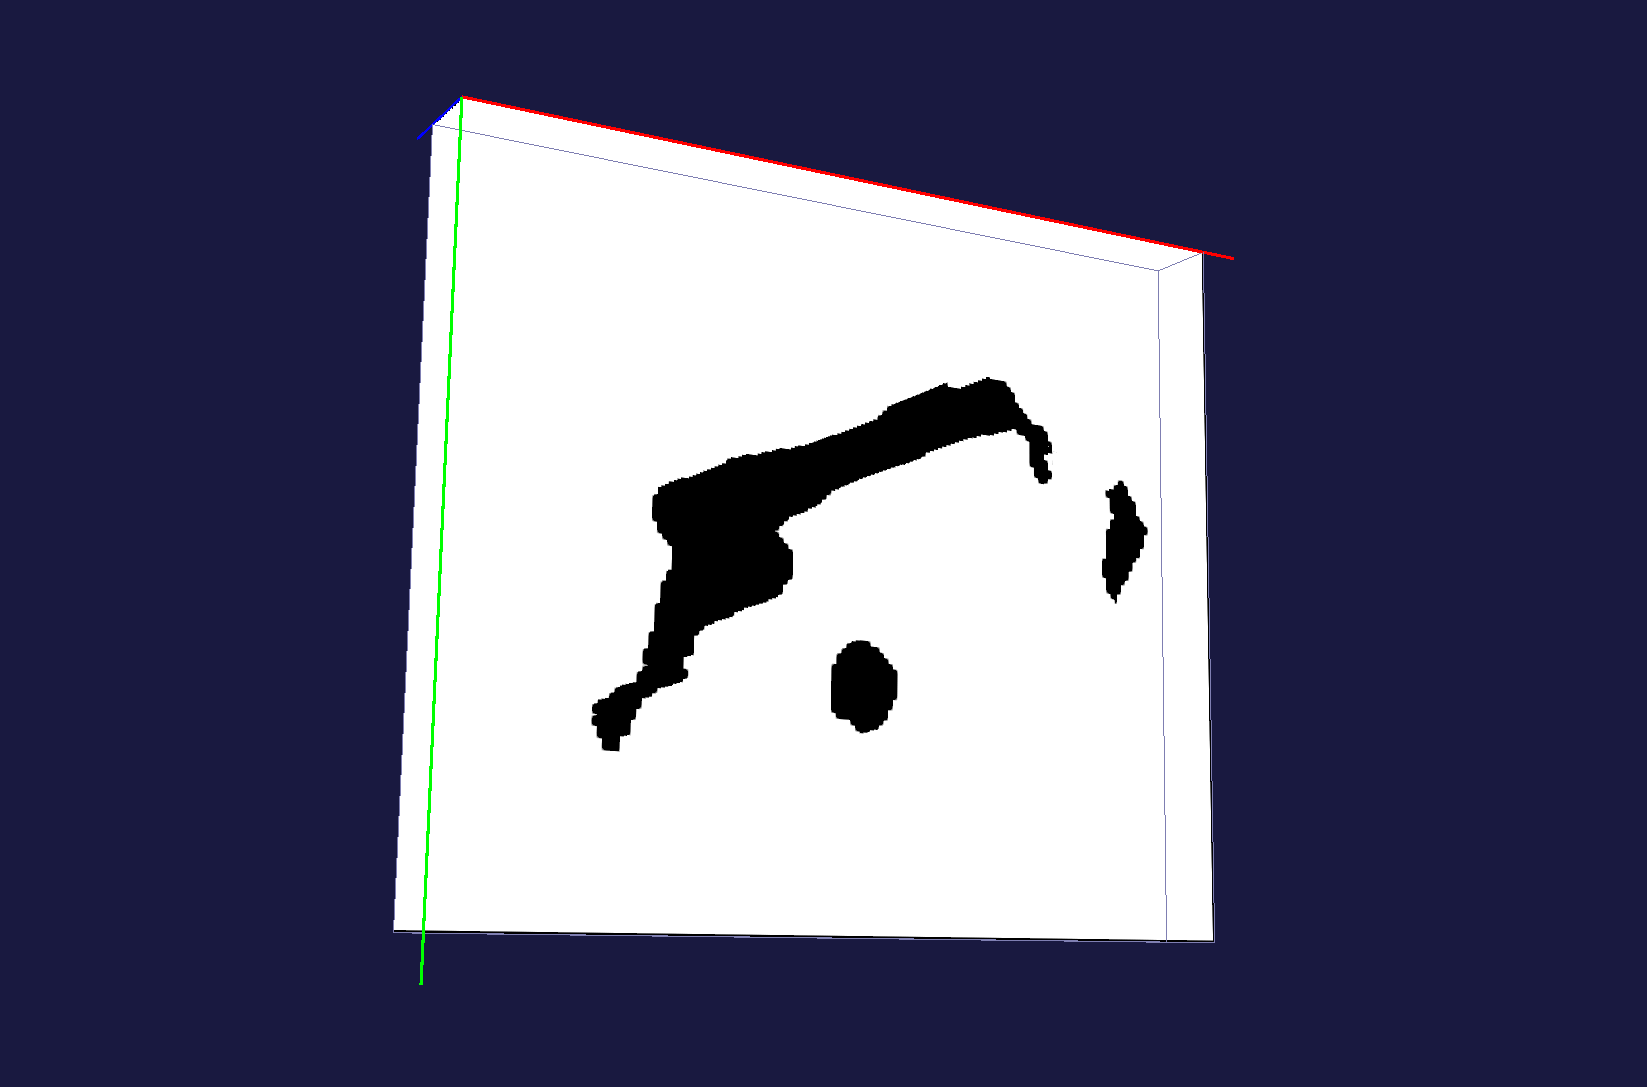
\includegraphics[width=0.45\textwidth]{Report/Images/6.3-7/BinaryImage_SurfaceVisualization_view2.png}}
\caption{Surface Visualization of the Binary Image}
\label{fig:binary-image-surface-viz}
\end{figure}

\clearpage
\section*{Question 4}
The acquired 3D images of zebrafish was first converted from  \textit{lif} to \textit{tiff} using the provided code snippet. It was loaded into Huygens and the microscopic parameters were set for all 4 images. 
The parameters were modified based on the notes taken during the lab session. 
\begin{figure}[h!]
    \centering
    \includegraphics[width=0.75\linewidth]{Report/Images/parameters_set.png}
    \caption{Microscopic Parameters}
    \label{fig:microscope-parameters}
\end{figure}
\subsection*{Static 3D Visualization}
The 3D visualization of the images was done using Huygens SFP Volume Renderer. The parameters were minimally modified, so as to show the untouched image. 
\begin{figure}[h!]
    \centering
    \includegraphics[width=0.75\linewidth]{Report/Images/6.4-9/Image_0.png}
    \caption{3D Visualization of Zebrafish}
    \label{fig:zebrafish_0}
\end{figure}
\begin{figure}[h!]
    \centering
    \includegraphics[width=0.75\linewidth]{Report/Images/6.4-9/image_1.png}
    \caption{3D Visualization of Zebrafish}
    \label{fig:zebrafish_1}
\end{figure}
\begin{figure}[h!]
    \centering
    \includegraphics[width=0.75\linewidth]{Report/Images/6.4-9/image_2.png}
    \caption{3D Visualization of Zebrafish}
    \label{fig:zebrafish_2}
\end{figure}
\begin{figure}[h!]
    \centering
    \includegraphics[width=0.75\linewidth]{Report/Images/6.4-9/image_3.png}
    \caption{3D Visualization of Zebrafish tail}
    \label{fig:zebrafish_tail}
\end{figure}
\subsection*{Improving Signal Strength}
For improving the signal strength, the channels of the image are separated, and 
\clearpage
\subsection*{Automated Deconvolution}
\subsubsection*{Image 1}
Image 1 was automatically deconvolved and the resultant image showed a significant improvement in SNR. Furthermore the reliability of the channels improved from fair-mediocre to very good.
\begin{figure}[h!]
\centering
\subfloat{\label{fig:Before Deconvolution 1}\includegraphics[width=0.45\textwidth]{Report/Images/original/Image_for_Huygens_0_rendering.jpg}}
\vspace{5 mm}
\subfloat{\label{fig:After Deconvolution 1}\includegraphics[width=0.45\textwidth]{Report/Images/deconvolved/Image_for_Huygens_0_decon_rendering.jpg}}
\caption{Automatic deconvolution of Image 1}
\label{fig:auto-deconvolve-image1}
\end{figure}
\begin{table}[h!]
\centering
\caption{Comparison of SNRs - Image 1 (reference : fig. \ref{fig:zebrafish_0})}
\begin{tabular}{*5c}
\toprule
Channel &  \multicolumn{2}{c}{Before Deconvolution} & \multicolumn{2}{c}{After Deconvolution}\\
\midrule
{}   & SNR   & Reliability    & SNR   & Reliability \\
0   &  15 & Very good   & 15.96  & Good\\
1   &  25 & Mediocre & 15.74  & Fair\\
2   &  16  &  Mediocre & 19.98  & Mediocre\\
\bottomrule
\end{tabular}
\end{table}
\subsubsection*{Image 2}
Similarly, image 2 was automatically deconvolved and the SNRs were noted. Though the image did not show any improvements in the SNR, further examination revealed that the intensities dropped slightly. 
\begin{figure}[h!]
\centering
\subfloat{\label{fig:Before Deconvolution 2}\includegraphics[width=0.45\textwidth]{Report/Images/original/Image_for_Huygens_1_rendering.jpg}}
\vspace{5 mm}
\subfloat{\label{fig:After Deconvolution 2}\includegraphics[width=0.45\textwidth]{Report/Images/deconvolved/Image_for_Huygens_1_decon_rendering.jpg}}
\caption{Automatic deconvolution of Image 2}
\label{fig:auto-deconvolve-image2}
\end{figure}
\begin{table}[h!]
\centering
\caption{Comparison of SNRs - Image 2 (reference : fig. \ref{fig:zebrafish_1})}
\begin{tabular}{*5c}
\toprule
Channel &  \multicolumn{2}{c}{Before Deconvolution} & \multicolumn{2}{c}{After Deconvolution}\\
\midrule
{}   & SNR   & Reliability    & SNR   & Reliability \\
0   &  16 & Very Good & 16 & Very Good \\
1   &  16 & Very Good & 16 & Very Good \\
2   &  16 & Very Good & 16 & Very Good \\
\bottomrule
\end{tabular}
\end{table}
\subsubsection*{Image 3}
Image 3 was automatically deconvolved and the SNRs were noted. Though the image did not show any improvements in the SNR (as the previous one), further examination revealed that the intensities dropped slightly. 
\begin{figure}[h!]
\centering
\subfloat{\label{fig:Before Deconvolution 3}\includegraphics[width=0.45\textwidth]{Report/Images/original/Image_for_Huygens_2_rendering.jpg}}
\vspace{5 mm}
\subfloat{\label{fig:After Deconvolution 3}\includegraphics[width=0.45\textwidth]{Report/Images/deconvolved/Image_for_Huygens_2_decon_rendering.jpg}}
\caption{Automatic deconvolution of Image 3}
\label{fig:auto-deconvolve-image3}
\end{figure}
\begin{table}[h!]
\centering
\caption{Comparison of SNRs - Image 3 (reference : fig. \ref{fig:zebrafish_2})}
\begin{tabular}{*5c}
\toprule
Channel &  \multicolumn{2}{c}{Before Deconvolution} & \multicolumn{2}{c}{After Deconvolution}\\
\midrule
{}   & SNR   & Reliability    & SNR   & Reliability \\
0   &  16 & Very Good & 16 & Very Good \\
1   &  16 & Very Good & 16 & Very Good \\
2   &  16 & Very Good & 16 & Very Good \\
\bottomrule
\end{tabular}
\end{table}
\subsubsection*{Image 4}
Image 4 (the zebrafish tail) was automatically deconvolved and the SNRs were noted. Though the image did not show any improvements in the SNR (as the previous ones), further examination revealed that the intensities dropped slightly. 
\begin{figure}[h!]
\centering
\subfloat{\label{fig:Before Deconvolution 4}\includegraphics[width=0.45\textwidth]{Report/Images/original/Image_for_Huygens_3_rendering.jpg}}
\vspace{5 mm}
\subfloat{\label{fig:After Deconvolution 4}\includegraphics[width=0.45\textwidth]{Report/Images/deconvolved/Image_for_Huygens_3_decon_rendering.jpg}}
\caption{Automatic deconvolution of Image 4}
\label{fig:auto-deconvolve-image4}
\end{figure}
\begin{table}[h!]
\centering
\caption{Comparison of SNRs - Image 4 (reference : fig. \ref{fig:zebrafish_tail})}
\begin{tabular}{*5c}
\toprule
Channel &  \multicolumn{2}{c}{Before Deconvolution} & \multicolumn{2}{c}{After Deconvolution}\\
\midrule
{}   & SNR   & Reliability    & SNR   & Reliability \\
0   &  16 & Very Good & 16 & Very Good \\
1   &  16 & Very Good & 16 & Very Good \\
2   &  16 & Very Good & 16 & Very Good \\
\bottomrule
\end{tabular}
\end{table}
\subsection*{Manual Deconvolution}
\subsection*{Visualizations}
\clearpage
\section*{Appendix}
\subsection*{Function to display image content in planes}
\begin{figure}[h!]
    \centering
    \includegraphics[width=1\linewidth]{Report/Images/3d_plot.png}
    \caption{The results of the function to display slices of tif image}
    \label{fig:3d-plane-image}
\end{figure}
% \bibliographystyle{alpha}
% \bibliography{sample}

\end{document}